% !TEX encoding = IsoLatin
%% LyX 2.0.2 created this file.  For more info, see http://www.lyx.org/.
%% Do not edit unless you really know what you are doing.
\documentclass[oneside,english]{book}
\usepackage[T1]{fontenc}
\usepackage[latin1]{inputenc}
\usepackage[letterpaper]{geometry}
\geometry{verbose,tmargin=1in,bmargin=1in,lmargin=1in,rmargin=1in}
\setcounter{secnumdepth}{3}
\setcounter{tocdepth}{3}
\usepackage{babel}
\usepackage{float}
\usepackage{textcomp}
\usepackage{url}
\usepackage{amsmath}
\usepackage{amssymb}
\usepackage{graphicx}
\usepackage[authoryear]{natbib}
\usepackage[unicode=true,pdfusetitle,
 bookmarks=true,bookmarksnumbered=true,bookmarksopen=false,
 breaklinks=false,pdfborder={0 0 0},backref=section,colorlinks=false,pdfpagemode=None]
 {hyperref}
\hypersetup{
 pdftex,pdfstartview=FitH,pdfpagelayout=SinglePage}
\usepackage{breakurl}

\makeatletter

%%%%%%%%%%%%%%%%%%%%%%%%%%%%%% LyX specific LaTeX commands.
\newcommand{\noun}[1]{\textsc{#1}}

%%%%%%%%%%%%%%%%%%%%%%%%%%%%%% Textclass specific LaTeX commands.
\newenvironment{lyxcode}
{\par\begin{list}{}{
\setlength{\rightmargin}{\leftmargin}
\setlength{\listparindent}{0pt}% needed for AMS classes
\raggedright
\setlength{\itemsep}{0pt}
\setlength{\parsep}{0pt}
\normalfont\ttfamily}%
 \item[]}
{\end{list}}
\newenvironment{lyxlist}[1]
{\begin{list}{}
{\settowidth{\labelwidth}{#1}
 \setlength{\leftmargin}{\labelwidth}
 \addtolength{\leftmargin}{\labelsep}
 \renewcommand{\makelabel}[1]{##1\hfil}}}
{\end{list}}

%%%%%%%%%%%%%%%%%%%%%%%%%%%%%% User specified LaTeX commands.
%\renewcommand{\baselinestretch}{1.5}

% figures
\usepackage[dvips]{epsfig}




% fonts
\usepackage{times}

% hyperlinks to sections and references


\newcommand{\urlwithparentheses}[1]{(\url{#1})}

% biblio GJI
\bibliographystyle{abbrvnat}

\newcommand{\toall}[1]{\textbf{*** All: #1 ***}}
\newcommand{\tojeroen}[1]{\textbf{*** Jeroen: #1 ***}}
\newcommand{\tobrian}[1]{\textbf{*** Brian: #1 ***}}
\newcommand{\tovala}[1]{\textbf{*** Vala: #1 ***}}
\newcommand{\tovalabrian}[1]{\textbf{*** Vala \& Brian: #1 ***}}
\newcommand{\tovalaqinya}[1]{\textbf{*** Vala \& Qinya: #1 ***}}
\newcommand{\toqinya}[1]{\textbf{*** Qinya: #1 ***}}
\newcommand{\tomin}[1]{\textbf{*** Min: #1 ***}}
\newcommand{\toalessia}[1]{\textbf{*** Alessia: #1 ***}}
\newcommand{\todimitri}[1]{\textbf{*** Dimitri: #1 ***}}

\newcommand{\nexxi}{\mbox{\texttt{NEX\_XI\/}}}
\newcommand{\nexeta}{\mbox{\texttt{NEX\_ETA\/}}}
\newcommand{\nprocxi}{\mbox{\texttt{NPROC\_XI\/}}}
\newcommand{\nproceta}{\mbox{\texttt{NPROC\_ETA\/}}}
\newcommand{\nchunks}{\mbox{\texttt{NCHUNKS\/}}}
\newcommand{\eg}{e.g.,}

% colors for the text
\@ifundefined{definecolor}
 {\usepackage{color}}{}
\newcommand{\red}[1]{\textcolor{Red}{#1}}

\usepackage{babel}

\makeatother

\begin{document}
\begin{center}
\thispagestyle{empty}\vspace*{-1.8truecm} %
\makebox[1\textwidth]{%
\includegraphics[width=0.83\paperwidth]{figures/specfem_3d_Cartesian-cover} %
}
\par\end{center}


\title{\textbf{SPECFEM3D Cartesian}\\
 \textbf{User Manual}}


\author{$\copyright$ Princeton University (USA), CNRS and University of Marseille (France),\\
and ETH Z\"urich (Switzerland)\\
Version 2.1}


\date{\today}

\maketitle

\section*{Authors}

\noindent The SPECFEM3D Cartesian package was first developed by Dimitri
Komatitsch and Jean-Pierre Vilotte at Institut de Physique du Globe
(IPGP) in Paris, France from 1995 to 1997 and then by Dimitri Komatitsch
and Jeroen Tromp at Harvard University and Caltech, USA, starting
in 1998. The story started on March 28, 1995, when Prof. Yvon Maday
from CNRS and University of Paris, France, gave a lecture to Dimitri
Komatitsch and Jean-Pierre Vilotte at IPG about the nice properties
of the spectral-element method that he had used for other equations.
We are deeply indebted and thankful to him for that.

Since then it has been developed and maintained by a development team:
in alphabetical order, Jean-Paul (Pablo) Ampuero, Piero Basini, C�line
Blitz, Ebru Bozda\u{g}, Emanuele Casarotti, Joseph Charles, Min Chen,
Percy Galvez, Dominik G�ddeke, Vala Hj�rleifsd�ttir, Sue Kientz, Dimitri
Komatitsch, Jes�s Labarta, Nicolas Le Goff, Pieyre Le Loher, Matthieu
Lefebvre, Qinya Liu, Yang Luo, Alessia Maggi, Federica Magnoni, Roland
Martin, Ren� Matzen, Dennis McRitchie, Matthias Meschede, Peter Messmer, 
David Mich�a, Surendra Nadh Somala, Tarje Nissen-Meyer, Daniel Peter, Max
Rietmann, Elliott Sales de Andrade, Brian Savage, Bernhard Schuberth,
Anne Sieminski, Leif Strand, Carl Tape, Jeroen Tromp, Jean-Pierre
Vilotte, Zhinan Xie, Hejun Zhu.\\


The cover graphic of the manual was created by Santiago Lombeyda from
Caltech's Center for Advanced Computing Research (CACR) \urlwithparentheses{http://www.cacr.caltech.edu}.
\\

\section*{Current and past main participants or main sponsors}

\begin{figure}[htbp]
\noindent \begin{centering}

\includegraphics[width=0.125\textwidth]{figures/logo_cnrs}\vspace*{2truemm}

\includegraphics[width=0.125\textwidth]{figures/logo_princeton}\vspace*{2truemm}

\includegraphics[width=0.15\textwidth]{figures/logo_aix_marseille_universite}\vspace*{0.02truemm}

\includegraphics[width=0.12\textwidth]{figures/logo_CSC_China}\vspace*{0.02truemm}

\includegraphics[width=0.15\textwidth]{figures/logo_ETH}\vspace*{2truemm}

\includegraphics[width=0.15\textwidth]{figures/logo_inria}\vspace*{2truemm}

\includegraphics[width=0.14\textwidth]{figures/logo_UPPA}
\par\end{centering}

\noindent \begin{centering}

\includegraphics[width=0.15\textwidth]{figures/logo_NVIDIA}\vspace*{2truemm}

\includegraphics[width=0.125\textwidth]{figures/logo_IUF}\vspace*{2truemm}

\includegraphics[width=0.135\textwidth]{figures/logo_Caltech}\vspace*{2truemm}

\includegraphics[width=0.135\textwidth]{figures/logo_Harvard}\vspace*{2truemm}

\includegraphics[width=0.135\textwidth]{figures/logo_IPGP}\vspace*{2truemm}
\par\end{centering}

\noindent \begin{centering}

\includegraphics[width=0.119\textwidth]{figures/logo_INGV}\vspace*{2truemm}

\includegraphics[width=0.119\textwidth]{figures/logo_University_of_Toronto}\vspace*{2truemm}

\includegraphics[width=0.112\textwidth]{figures/logo_Univ_Toulouse}\vspace*{2truemm}

\includegraphics[width=0.112\textwidth]{figures/logo_TOTAL}\vspace*{2truemm}

\includegraphics[width=0.130\textwidth]{figures/logo_Fairbanks}
\hspace*{3mm}
\includegraphics[width=0.130\textwidth]{figures/logo_fondation_Del_Duca}
\par\end{centering}
\end{figure}

\newpage{}

\tableofcontents{}


\chapter{Introduction}

The software package SPECFEM3D Cartesian simulates seismic wave propagation
at the local or regional scale based upon the spectral-element method
(SEM). The SEM is a continuous Galerkin technique \citep{TrKoLi08,PeKoLuMaLeCaLeMaLiBlNiBaTr11},
which can easily be made discontinous \citep{BeMaPa94,Ch00,KoWoHu02,ChCaVi03,LaWaBe05,Kop06,WiStBuGh10,AcKo11};
it is then close to a particular case of the discontinuous Galerkin
technique \citep{ReHi73,LeRa74,Arn82,JoPi86,BoMaHe91,FaRi99,HuHuRa99,CoKaSh00,GiHeWa02,RiWh03,MoRi05,GrScSc06,AiMoMu06,BeLaPi06,DuKa06,DeSeWh08,PuAmKa09,WiStBuGh10,DeSe10,EtChViGl10},
with optimized efficiency because of its tensorized basis functions
\citep{WiStBuGh10,AcKo11}. In particular, it can accurately handle
very distorted mesh elements \citep{OlSe11}.\\


It has very good accuracy and convergence properties \citep{MaPa89,SePr94,DeFiMu02,Coh02,DeSe07,SeOl08,AiWa09,AiWa10,MeStTh12}.
The spectral element approach admits spectral rates of convergence
and allows exploiting $hp$-convergence schemes. It is also very well
suited to parallel implementation on very large supercomputers \citep{KoTsChTr03,TsKoChTr03,KoLaMi08a,CaKoLaTiMiLeSnTr08,KoViCh10}
as well as on clusters of GPU accelerating graphics cards \citep{Kom11,MiKo10,KoMiEr09,KoErGoMi10}.
Tensor products inside each element can be optimized to reach very
high efficiency \citep{DeFiMu02}, and mesh point and element numbering
can be optimized to reduce processor cache misses and improve cache
reuse \citep{KoLaMi08a}. The SEM can also handle triangular (in 2D)
or tetrahedral (in 3D) elements \citep{WinBoyd96,TaWi00,KoMaTrTaWi01,Coh02,MeViSa06}
as well as mixed meshes, although with increased cost and reduced
accuracy in these elements, as in the discontinuous Galerkin method.\\


Note that in many geological models in the context of seismic wave
propagation studies (except for instance for fault dynamic rupture
studies, in which very high frequencies or supershear rupture need
to be modeled near the fault, see e.g. \citet{BeGlCrViPi07,BeGlCrVi09,PuAmKa09,TaCrEtViBeSa10})
a continuous formulation is sufficient because material property contrasts
are not drastic and thus conforming mesh doubling bricks can efficiently
handle mesh size variations \citep{KoTr02a,KoLiTrSuStSh04,LeChLiKoHuTr08,LeChKoHuTr09,LeKoHuTr09}.\\


For a detailed introduction to the SEM as applied to regional seismic
wave propagation, please consult \citet{PeKoLuMaLeCaLeMaLiBlNiBaTr11,TrKoLi08,KoVi98,KoTr99,ChKoViCaVaFe07}
and in particular \citet{LeKoHuTr09,LeChKoHuTr09,LeChLiKoHuTr08,GoAmTaCaSmSaMaKo09,WiKoScTr04,KoLiTrSuStSh04}.
A detailed theoretical analysis of the dispersion
and stability properties of the SEM is available in \citet{Coh02}, \citet{DeSe07}, \citet{SeOl07}, \citet{SeOl08} and \citet{MeStTh12}.\\


Effects due to lateral variations in compressional-wave speed, shear-wave
speed, density, a 3D crustal model, topography and bathymetry are
included. The package can accommodate full 21-parameter anisotropy
(see~\citet{ChTr07}) as well as lateral variations in attenuation
\citep{SaKoTr10}. Adjoint capabilities and finite-frequency kernel
simulations are included \citep{TrKoLi08,PeKoLuMaLeCaLeMaLiBlNiBaTr11,LiTr06,FiIgBuKe09,ViOp09}.\\


The SEM was originally developed in computational fluid dynamics \citep{Pat84,MaPa89}
and has been successfully adapted to address problems in seismic wave
propagation. Early seismic wave propagation applications of the SEM,
utilizing Legendre basis functions and a perfectly diagonal mass matrix,
include \citet{CoJoTo93}, \citet{Kom97}, \citet{FaMaPaQu97}, \citet{CaGa97},
\citet{KoVi98} and \citet{KoTr99}, whereas applications involving
Chebyshev basis functions and a nondiagonal mass matrix include \citet{SePr94},
\citet{PrCaSe94} and \citet{SePrPr95}.\\


All SPECFEM3D software is written in Fortran2003 with full portability
in mind, and conforms strictly to the Fortran2003 standard. It uses
no obsolete or obsolescent features of Fortran. The package uses parallel
programming based upon the Message Passing Interface (MPI) \citep{GrLuSk94,Pac97}.\\


SPECFEM3D won the Gordon Bell award for best performance at the SuperComputing~2003
conference in Phoenix, Arizona (USA) (see \citet{KoTsChTr03} and
\url{www.sc-conference.org/sc2003/nrfinalaward.html}). It was a finalist
again in 2008 for a run at 0.16 petaflops (sustained) on 149,784 processors
of the `Jaguar' Cray XT5 system at Oak Ridge National Laboratories
(USA) \citep{CaKoLaTiMiLeSnTr08}. It also won the BULL Joseph Fourier
supercomputing award in 2010.\\

It reached the sustained one petaflop performance level for the first time in February 2013
on the Blue Waters Cray supercomputer at the National Center for Supercomputing Applications (NCSA), located at the University of Illinois at Urbana-Champaign (USA).\\


This new release of the code (version 2.1) includes Convolution or
Auxiliary Differential Equation Perfectly Matched absorbing Layers
(C-PML or ADE-PML) \citep{MaKoEz08,MaKoGe08,MaKo09,MaKoGeBr10,KoMa07}.
It also includes support for GPU graphics card acceleration \citep{Kom11,MiKo10,KoMiEr09,KoErGoMi10}.\\


The next release of the code will use the PT-SCOTCH parallel and threaded
version of SCOTCH for mesh partitioning instead of the serial version.\\


SPECFEM3D Cartesian includes coupled fluid-solid domains and adjoint
capabilities, which enables one to address seismological inverse problems,
but for linear rheologies only so far. To accommodate visco-plastic
or non-linear rheologies, the reader can refer to the \href{http://geoelse.stru.polimi.it/}{GeoELSE}software
package \citep{CaGa97,StPaIg09}.


\section{Citation}

If you use SPECFEM3D Cartesian for your own research, please cite
at least one of the following articles:
\begin{description}
\item [{Numerical simulations in general}] ~\\
 Forward and adjoint simulations are described in detail in \citet{TrKoLi08,PeKoLuMaLeCaLeMaLiBlNiBaTr11,VaCaSaKoVi99,KoMiEr09,KoErGoMi10,ChKoViCaVaFe07,MaKoDi09,KoViCh10,CaKoLaTiMiLeSnTr08,TrKoHjLiZhPeBoMcFrTrHu10,KoRiTr02,KoTr02a,KoTr02b,KoTr99}
or \citet{KoVi98}. Additional aspects of adjoint simulations are
described in \citet{TrTaLi05,LiTr06,TrKoLi08,LiTr08,TrKoHjLiZhPeBoMcFrTrHu10,PeKoLuMaLeCaLeMaLiBlNiBaTr11}.
Domain decomposition is explained in detail in \citet{MaKoBlLe08},
and excellent scaling up to 150,000 processor cores is shown for instance
in \citet{CaKoLaTiMiLeSnTr08,KoLaMi08a,MaKoBlLe08,KoErGoMi10,Kom11},
\item [{GPU computing}] ~\\
 Computing on GPU graphics cards for acoustic or seismic wave propagation
applications is described in detail in \citet{Kom11,MiKo10,KoMiEr09,KoErGoMi10}.
\end{description}
\noindent If you use this new version 2.1, which has non blocking
MPI for much better performance for medium or large runs, please cite
at least one of these six articles, in which results of non blocking
MPI runs are presented: \citet{PeKoLuMaLeCaLeMaLiBlNiBaTr11,KoErGoMi10,KoViCh10,Kom11,CaKoLaTiMiLeSnTr08,MaKoBlLe08}.\\


\noindent If you work on geophysical applications, you may be interested
in citing some of these application articles as well, among others:
\begin{description}
\item [{Southern California simulations}] ~\\
 \citet{KoLiTrSuStSh04,KrJiKoTr06a,KrJiKoTr06b}.


If you use the 3D southern California model, please cite \citet{SuSh03}
(Los Angeles model), \citet{lovelyetal06} (Salton Trough), and \citet{hauksson2000}
(southern California). The Moho map was determined by \citet{zhu&kanamori2000}.
The 1D SoCal model was developed by \citet{DrHe90}.

\item [{Anisotropy}] ~\\
 \citet{ChTr07,JiTsKoTr05,ChFaKo04,FaChKo04,RiRiKoTrHe02,TrKo00}.
\item [{Attenuation}] ~\\
 \citet{SaKoTr10,KoTr02a,KoTr99}.
\item [{Topography}] ~\\
 \citet{LeKoHuTr09,LeChKoHuTr09,LeChLiKoHuTr08,GoAmTaCaSmSaMaKo09,WiKoScTr04}.
\end{description}
The corresponding Bib\TeX{} entries may be found in file \texttt{doc/USER\_MANUAL/bibliography.bib}.


\section{Support}

This material is based upon work supported by the USA National Science
Foundation under Grants No. EAR-0406751 and EAR-0711177, by the French
CNRS, French INRIA Sud-Ouest MAGIQUE-3D, French ANR NUMASIS under
Grant No. ANR-05-CIGC-002, and European FP6 Marie Curie International
Reintegration Grant No. MIRG-CT-2005-017461. Any opinions, findings,
and conclusions or recommendations expressed in this material are
those of the authors and do not necessarily reflect the views of the
USA National Science Foundation, CNRS, INRIA, ANR or the European
Marie Curie program.


\chapter{\label{cha:Getting-Started}Getting Started}

To download the SPECFEM3D\_Cartesian software package, type this:
\begin{lyxcode}
git clone --recursive --branch devel https://github.com/geodynamics/specfem3d.git
\end{lyxcode}
{\small \par}

We recommend that you add {\texttt{ulimit -S -s unlimited}} to your
{\texttt{.bash\_profile}} file and/or {\texttt{limit stacksize
unlimited }} to your {\texttt{.cshrc}} file to suppress any potential
limit to the size of the Unix stack.\\


Then, to configure the software for your system, run the \texttt{configure}
shell script. This script will attempt to guess the appropriate configuration
values for your system. However, at a minimum, it is recommended that
you explicitly specify the appropriate command names for your Fortran
compiler and MPI package (another option is to define FC, CC and MPIF90
in your .bash\_profile or your .cshrc file):
\begin{lyxcode}
./configure~FC=ifort~MPIFC=mpif90
\end{lyxcode}
Before running the \texttt{configure} script, you should probably
edit file \texttt{flags.guess} to make sure that it contains the best
compiler options for your system. Known issues or things to check
are:
\begin{description}
\item [{\texttt{Intel ifort compiler}}] See if you need to add \texttt{-assume
byterecl} for your machine.
\item [{\texttt{IBM compiler}}] See if you need to add \texttt{-qsave}
or \texttt{-qnosave} for your machine.
\item [{\texttt{Mac OS}}] You will probably need to install \texttt{XCODE}.
In addition, the \texttt{clock\_gettime} routine, which is used by
the \texttt{SCOTCH} library that we use, does not exist in Mac OS.
You will need to replace it with \texttt{clock\_get\_time} if you
want to use \texttt{SCOTCH}.
\end{description}
When compiling on an IBM machine with the \texttt{xlf} and \texttt{xlc}
compilers, we suggest running the \texttt{configure} script with the
following options:\\


\noindent \texttt{./configure FC=xlf90\_r MPIFC=mpif90 CC=xlc\_r CFLAGS=\textquotedbl{}-O3
-q64\textquotedbl{} FCFLAGS=\textquotedbl{}-O3 -q64\textquotedbl{}
-with-scotch-dir=...}.\\


On SGI systems, \texttt{flags.guess} automatically informs \texttt{configure}
to insert `\texttt{`TRAP\_FPE=OFF}'' into the generated \texttt{Makefile}
in order to turn underflow trapping off.\\

You can add -DFORCE\_VECTORIZATION to the compiler options in \texttt{flags.guess} (for all compilers, except for IBM for which the syntax is -WF,-DFORCE\_VECTORIZATION )
to speed up the code in the fluid (acoustic) parts (only; FORCE\_VECTORIZATION support for elastic parts has been discontinued in the source code).
This works fine if (and only if) your computer always allocates a contiguous memory block for each allocatable array;
this is the case for most machines and most compilers, but not all. For more details see https://github.com/geodynamics/specfem3d/issues/81 .
To check if that option works fine on your machine, run the code with and without it for a model containing a significant fluid layer
(or entirely fluid) and make sure the seismograms are identical.\\

Note that we use CUBIT (now called Trelis) to create meshes of hexahedra, but other packages
can be used as well, for instance GiD from \url{http://gid.cimne.upc.es}
or Gmsh from \url{http://geuz.org/gmsh} \citep{GeRe09}. Even mesh
creation packages that generate tetrahedra, for instance TetGen from
\url{http://tetgen.berlios.de}, can be used because each tetrahedron
can then easily be decomposed into four hexahedra as shown in the
picture of the TetGen logo at \url{http://tetgen.berlios.de/figs/Delaunay-Voronoi-3D.gif};
while this approach does not generate hexahedra of optimal quality,
it can ease mesh creation in some situations and it has been shown
that the spectral-element method can very accurately handle distorted
mesh elements \citep{OlSe11}.

The SPECFEM3D Cartesian software package relies on the SCOTCH library
to partition meshes created with CUBIT. METIS \citep{KaKu98a,KaKu98c,KaKu98b}
can also be used instead of SCOTCH if you prefer, by editing file
src/decompose\_mesh/decompose\_mesh.F90 and uncommenting the flag
USE\_METIS\_INSTEAD\_OF\_SCOTCH. You will also then need to install
and compile Metis version 4.0 (do {*}NOT{*} install Metis version
5.0, which has incompatible function calls) and edit \texttt{src/decompose\_mesh/Makefile.in}
and uncomment the METIS link flag in that file before running \texttt{configure}.\\


The SCOTCH library \citep{PeRo96} provides efficent static mapping,
graph and mesh partitioning routines. SCOTCH is a free software package
developed by Fran�ois Pellegrini et al. from LaBRI and INRIA in Bordeaux,
France, downloadable from the web page \url{https://gforge.inria.fr/projects/scotch/}.
In case no SCOTCH libraries can be found on the system, the configuration
will bundle the version provided with the source code for compilation.
The path to an existing SCOTCH installation can to be set explicitly
with the option \texttt{-{}-with-scotch-dir}. Just as an example:
\begin{lyxcode}
./configure~FC=ifort~MPIFC=mpif90~-{}-with-scotch-dir=/opt/scotch
\end{lyxcode}
If you use the Intel ifort compiler to compile the code, we recommend
that you use the Intel icc C compiler to compile Scotch, i.e., use:
\begin{lyxcode}
./configure~CC=icc~FC=ifort~MPIFC=mpif90
\end{lyxcode}

When compiling the SCOTCH source code, if you get a message such as: "ld: cannot find -lz",
the Zlib compression development library is probably missing on your machine and you will need to install it or ask your system administrator to 
do so. On Linux machines the package is often called "zlib1g-dev" or similar. (thus "sudo apt-get install zlib1g-dev" would install it)

To compile a serial version of the code for small meshes that fits
on one compute node and can therefore be run serially, run \texttt{configure}
with the \texttt{-{}-without-mpi} option to suppress all calls to
MPI.

A summary of the most important configuration variables follows.
\begin{description}
\item [{\texttt{F90}}] Path to the Fortran compiler.
\item [{\texttt{MPIF90}}] Path to MPI Fortran.
\item [{\texttt{MPI\_FLAGS}}] Some systems require this flag to link to
MPI libraries.
\item [{\texttt{FLAGS\_CHECK}}] Compiler flags.
\end{description}
The configuration script automatically creates for each executable
a corresponding \texttt{Makefile} in the \texttt{src/} subdirectoy.
The \texttt{Makefile} contains a number of suggested entries for various
compilers, e.g., Portland, Intel, Absoft, NAG, and Lahey. The software
has run on a wide variety of compute platforms, e.g., various PC clusters
and machines from Sun, SGI, IBM, Compaq, and NEC. Select the compiler
you wish to use on your system and choose the related optimization
flags. Note that the default flags in the \texttt{Makefile} are undoubtedly
not optimal for your system, so we encourage you to experiment with
these flags and to solicit advice from your systems administrator.
Selecting the right compiler and optimization flags can make a tremendous
difference in terms of performance. We welcome feedback on your experience
with various compilers and flags.

Now that you have set the compiler information, you need to select
a number of flags in the \texttt{constants.h} file depending on your
system:
\begin{description}
\item [{\texttt{LOCAL\_PATH\_IS\_ALSO\_GLOBAL}}] Set to \texttt{.false.}
on most cluster applications. For reasons of speed, the (parallel)
distributed database generator typically writes a (parallel) database
for the solver on the local disks of the compute nodes. Some systems
have no local disks, e.g., BlueGene or the Earth Simulator, and other
systems have a fast parallel file system, in which case this flag
should be set to \texttt{.true.}. Note that this flag is not used
by the database generator or the solver; it is only used for some
of the post-processing.
\end{description}
The package can run either in single or in double precision mode.
The default is single precision because for almost all calculations
performed using the spectral-element method using single precision
is sufficient and gives the same results (i.e. the same seismograms);
and the single precision code is faster and requires exactly half
as much memory. Select your preference by selecting the appropriate
setting in the \texttt{constants.h} file:
\begin{description}
\item [{\texttt{CUSTOM\_REAL}}] Set to \texttt{SIZE\_REAL} for single precision
and \texttt{SIZE\_DOUBLE} for double precision.
\end{description}
In the \texttt{precision.h} file:
\begin{description}
\item [{\texttt{CUSTOM\_MPI\_TYPE}}] Set to \texttt{MPI\_REAL} for single
precision and \texttt{MPI\_DOUBLE\_PRECISION} for double precision.
\end{description}
On many current processors (e.g., Intel, AMD, IBM Power), single precision
calculations are significantly faster; the difference can typically
be 10\% to 25\%. It is therefore better to use single precision. What
you can do once for the physical problem you want to study is run
the same calculation in single precision and in double precision on
your system and compare the seismograms. If they are identical (and
in most cases they will), you can select single precision for your
future runs.\\

If your compiler has problems with the \texttt{use mpi} statements that are used in the code, use the script called 
\texttt{replace\_use\_mpi\_with\_include\_mpif\_dot\_h.pl} in the root directory to replace all of them with \texttt{include 'mpif.h'} automatically.

\section{Adding OpenMP support in addition to MPI}

NOTE FROM JULY 2013: OpenMP support is maybe / probably not maintained any more.
Thus the section below is maybe obsolete.

OpenMP support can be enabled in addition to MPI. However, in many
cases performance will not improve because our pure MPI implementation
is already heavily optimized and thus the resulting code will in fact
be slightly slower. A possible exception could be IBM BlueGene-type
architectures.

To enable OpenMP, uncomment the OpenMP compiler option in two lines
in file \texttt{src/specfem3D/Makefile.in} (before running \texttt{configure})
and also uncomment the \texttt{\#define USE\_OPENMP} statement in
file\\
 \texttt{src/specfem3D/specfem3D.F90}.

The DO-loop using OpenMP threads has a SCHEDULE property. The OMP\_SCHEDULE
environment variable can set the scheduling policy of that DO-loop.
Tests performed by Marcin Zielinski at SARA (The Netherlands) showed
that often the best scheduling policy is DYNAMIC with the size of
the chunk equal to the number of OpenMP threads, but most preferably
being twice as the number of OpenMP threads (thus chunk size = 8 for
4 OpenMP threads etc). If OMP\_SCHEDULE is not set or is empty, the
DO-loop will assume generic scheduling policy, which will slow down
the job quite a bit.


\section{Compiling on an IBM BlueGene}

\underline{More recent installation instruction for IBM BlueGene, from April 2013:}\\


\noindent Edit file \texttt{flags.guess} and put this for \texttt{FLAGS\_CHECK}:\\


\noindent \texttt{-g -qfullpath -O2 -qsave -qstrict -qtune=qp -qarch=qp
-qcache=auto -qhalt=w}\\
 \texttt{-qfree=f90 -qsuffix=f=f90 -qlanglvl=95pure -Q -Q+rank,swap\_all
-Wl,-relax}\\


\noindent The most relevant are the -qarch and -qtune flags, otherwise
if these flags are set to ``auto'' then they are wrongly assigned
to the architecture of the frond-end node, which is different from
that on the compute nodes. You will need to set these flags to the
right architecture for your BlueGene compute nodes, which is not necessarily
``qp''; ask your system administrator. On some machines if is necessary
to use -O2 in these flags instead of -O3 due to a compiler bug of
the XLF version installed. We thus suggest to first try -O3, and then
if the code does not compile or does not run fine then switch back
to -O2. The debug flags (-g, -qfullpath) do not influence performance
but are useful to get at least some insights in case of problems.\\


\noindent Before running \texttt{configure}, select the XL Fortran
compiler by typing \texttt{module load bgq-xl/1.0} or \texttt{module
load bgq-xl} (another, less efficient option is to load the GNU compilers
using \texttt{module load bgq-gnu/4.4.6} or similar).\\


\noindent Then, to configure the code, type this:\\


\noindent \texttt{./configure FC=bgxlf90\_r MPIFC=mpixlf90\_r CC=bgxlc\_r
LOCAL\_PATH\_IS\_ALSO\_GLOBAL=true}\\


In order for the SCOTCH domain decomposer to compile, on some (but
not all) Blue Gene systems you may need to run \texttt{configure}
with \texttt{CC=gcc} instead of \texttt{CC=bgxlc\_r}.

\noindent \underline{Older installation instruction for IBM BlueGene, from 2011:}\\


\noindent To compile the code on an IBM BlueGene, Laurent L�ger from
IDRIS, France, suggests the following: compile the code with

\noindent \texttt{ FLAGS\_CHECK=\textquotedbl{}-O3 -qsave -qstrict
-qtune=auto -qarch=450d -qcache=auto }~\\
 \texttt{ -qfree=f90 -qsuffix=f=f90 -g -qlanglvl=95pure -qhalt=w -Q
-Q+rank,swap\_all -Wl,-relax\textquotedbl{}}

\noindent Option \textquotedbl{}-Wl,-relax\textquotedbl{} must be
added on many (but not all) BlueGene systems to be able to link the
binaries \texttt{xmeshfem3D} and \texttt{xspecfem3D} because the final
link step is done by the GNU \texttt{ld} linker even if one uses \texttt{FC=bgxlf90\_r,
MPIFC=mpixlf90\_r} and \texttt{CC=bgxlc\_r} to create all the object
files. On the contrary, on some BlueGene systems that use the native
AIX linker option \textquotedbl{}-Wl,-relax\textquotedbl{} can lead
to problems and must be suppressed from \texttt{flags.guess}.

\noindent Also, \texttt{AR=ar, ARFLAGS=cru} and \texttt{RANLIB=ranlib}
are hardwired in all \texttt{Makefile.in} files by default, but to
cross-compile on BlueGene/P one needs to change these values to \texttt{AR=bgar,
ARFLAGS=cru} and \texttt{RANLIB=bgranlib}. Thus the easiest thing
to do is to modify all \texttt{Makefile.in} files and the \texttt{configure}
script to set them automatically by \texttt{configure}. One then just
needs to pass the right commands to the \texttt{configure} script:

\noindent \texttt{ ./configure -{}-prefix=/path/to/SPECFEM3DG\_SP
-{}-host=Babel -{}-build=BGP }~\\
 \texttt{ FC=bgxlf90\_r MPIFC=mpixlf90\_r CC=bgxlc\_r AR=bgar ARFLAGS=cru
}~\\
 \texttt{ RANLIB=bgranlib LOCAL\_PATH\_IS\_ALSO\_GLOBAL=false}

\noindent This trick can be useful for all hosts on which one needs
to cross-compile.

\noindent On BlueGene, one also needs to run the \texttt{xcreate\_header\_file}
binary file manually rather than in the Makefile:

\noindent \texttt{bgrun -np 1 -mode VN -exe ./bin/xcreate\_header\_file}


\section{Visualizing the subroutine calling tree of the source code}

\noindent
Packages such as \texttt{Doxywizard} can be used to visualize the calling tree of the
subroutines of the  source code. \texttt{Doxywizard} is
a GUI front-end for configuring and running \texttt{Doxygen}.

\bigskip

\noindent To do your own call graphs, you can follow these simple steps below.

\begin{enumerate}
\setcounter{enumi}{-1}
\item Install \texttt{Doxygen} \underline{and} \texttt{graphviz} (the two are usually in the package manager of classic Linux distribution).
\item Run in the terminal : \texttt{doxygen -g}, which creates a \texttt{Doxyfile} that tells doxygen what you want it to do.
\item Edit the Doxyfile. Two Doxyfile-type files have been already committed in the directory \\
\noindent \texttt{specfem3d/doc/Call\_trees}:

\begin{itemize}
\item[\textbullet] \texttt{Doxyfile\_truncated\_call\_tree} will generate call graphs with maximum 3 or 4 levels of tree structure,
\item[\textbullet] \texttt{Doxyfile\_complete\_call\_tree} will generate call graphs with complete tree structure.
\end{itemize}

The important entries in the Doxyfile are:

\begin{description}
\item [{\texttt{PROJECT\_NAME}}] 
\item [{\texttt{OPTIMIZE\_FOR\_FORTRAN}}] Set to YES
\item [{\texttt{EXTRACT\_ALL}}] Set to YES
\item [{\texttt{EXTRACT\_PRIVATE}}] Set to YES
\item [{\texttt{EXTRACT\_STATIC}}] Set to YES
\item [{\texttt{INPUT}}] From the directory \texttt{specfem3d/doc/Call\_trees}, it is \texttt{"../../src/"}
\item [{\texttt{FILE\_PATTERNS}}] In SPECFEM case, it is \texttt{*.f90* *.F90* *.c* *.cu* *.h*}
\item [{\texttt{HAVE\_DOT}}] Set to YES
\item [{\texttt{CALL\_GRAPH}}] Set to YES
\item [{\texttt{CALLER\_GRAPH}}] Set to YES
\item [{\texttt{DOT\_PATH}}] The path where is located the dot program graphviz (if it is not in your \$PATH)
\item [{\texttt{RECURSIVE}}] This tag can be used to turn specify whether or not subdirectories should be searched for input files as well. In the case of SPECFEM, set to YES.
\item [{\texttt{EXCLUDE}}] Here, you can exclude:  \\
\texttt{"../../src/specfem3D/older\_not\_maintained\_partial\_OpenMP\_port"}\\
\texttt{"../../src/decompose\_mesh/scotch"}\\
\texttt{"../../src/decompose\_mesh/scotch\_5.1.12b"}
\item [{\texttt{DOT\_GRAPH\_MAX\_NODES}}] to set the maximum number of nodes that will be shown in the graph. If the number of nodes in a graph becomes larger than this value, doxygen will truncate the graph, which is visualized by representing a node as a red box. Minimum value: 0, maximum value: 10000, default value: 50.
\item [{\texttt{MAX\_DOT\_GRAPH\_DEPTH}}] to set the maximum depth of the graphs generated by dot. A depth value of 3 means that only nodes reachable from the root by following a path via at most 3 edges will be shown. Using a depth of 0 means no depth restriction. Minimum value: 0, maximum value: 1000, default value: 0.

\end{description}

\item Run : \texttt{doxygen Doxyfile}, HTML and LaTeX files created by default in \texttt{html} and \texttt{latex} subdirectories.

\item To see the call trees, you have to open the file \texttt{html/index.html} in your \underline{browser}. You will have many informations about each subroutines of SPECFEM (not only call graphs), you can click on every boxes / subroutines. It show you the call, and, the caller graph of each subroutine : the subroutines called by the concerned subroutine, and the previous subroutines who call this subroutine (the previous path), respectively. In the case of a truncated calling tree, the boxes with a red border indicates a node that has \underline{more} arrows than are shown (in other words: the graph is truncated with respect to this node). 

\end{enumerate}

\medskip

\noindent Finally, some useful links: 

\begin{itemize}
\item[\textbullet] a good and short summary for the basic utilisation of Doxygen:

\texttt{http://www.softeng.rl.ac.uk/blog/2010/jan/30/callgraph-fortran-doxygen/} ,

\item[\textbullet] to configure the diagrams : 

\texttt{http://www.stack.nl/~dimitri/doxygen/manual/diagrams.html} ,

\item[\textbullet] the complete alphabetical index of the tags in Doxyfile: 

\texttt{http://www.stack.nl/~dimitri/doxygen/manual/config.html} ,

\item[\textbullet] more generally, the Doxygen manual:

\texttt{http://www.stack.nl/~dimitri/doxygen/manual/index.html} .

\end{itemize}

\medskip

\section{Using the ADIOS library for I/O}
Regular POSIX I/O can be problematic when dealing with large simulations one large
clusters (typically more than $10,000$ processes). SPECFEM3D use the ADIOS library~\cite{Liu2013}
to deal transparently take advantage of advanced paralllel file system features. To enable
ADIOS, the following steps should be done:
\begin{enumerate}
\item Install ADIOS (available from \url{https://www.olcf.ornl.gov/center-projects/adios/}). 
Make sure that your environment variables reference it. 
\item You may want to change ADIOS related values in the \texttt{constants.h.in} file.
The default values probably suit most cases.
\item Configure using the \texttt{--with-adios} flag.
\end{enumerate}
ADIOS is currently only usable for meshfem3D generated mesh (i.e. not for meshes generated
with CUBTI). Additional control parameters are discussed in section~\ref{cha:Main-Parameter}.

%%%%%%%%%%%%%%%%%%%%%%%%%%%%%%%%%%%%%%%%%%%%%%%%%%%%%%%%%%%%%%%%%%%%%%%%%%%%%%%%%%%%%



\chapter{\label{cha:Mesh-Generation}Mesh Generation}

The first step in running a spectral-element simulation consists of
constructing a high-quality mesh for the region under consideration.
We provide two possibilities to do so: (1) relying on the external,
hexahedral mesher CUBIT, or (2) using the provided, internal mesher
\texttt{xmeshfem3D}. In the following, we explain these two approaches.


\section{\label{cha:Running-the-Mesher-CUBIT}Meshing with \texttt{CUBIT}}

CUBIT is a meshing tool suite for the creation of finite-element meshes
for arbitrarily shaped models. It has been developed and maintained
at Sandia National Laboratories and can be purchased for a small academic
institutional fee at \url{http://cubit.sandia.gov}. Our experience
showed that using CUBIT greatly facilitates and speeds up the generation
and preparation of hexahedral, conforming meshes for a variety of
geophysical models with increasing complexity.

\begin{figure}[htbp]
\noindent \begin{centering}
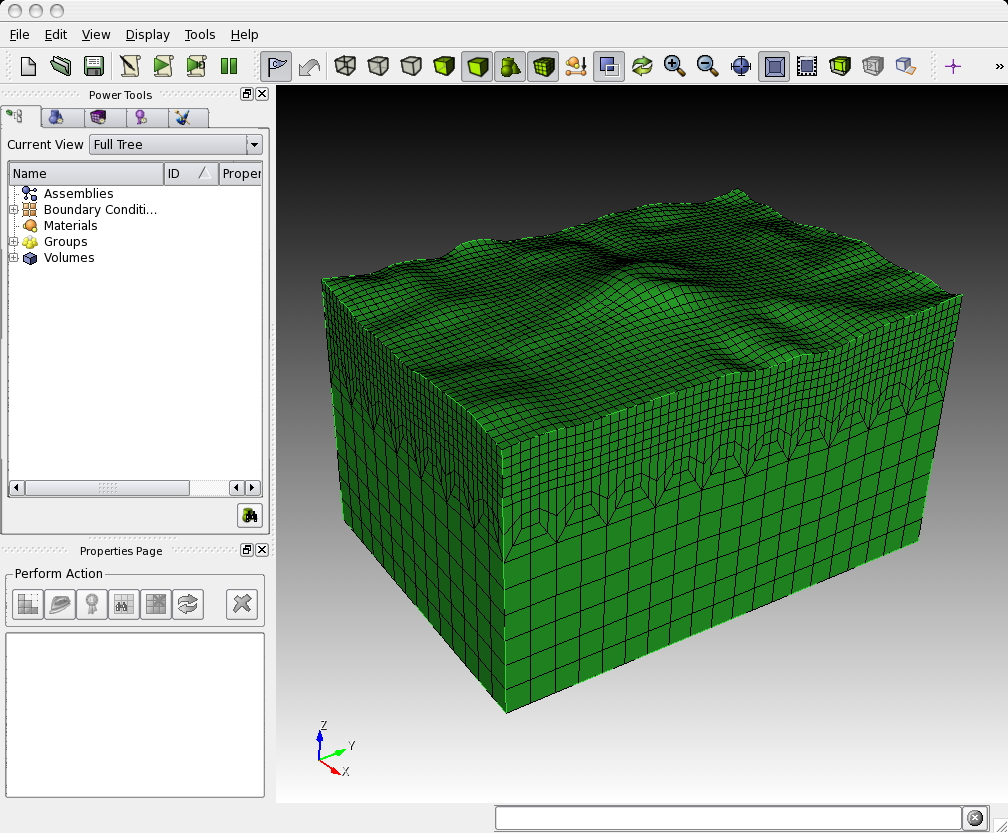
\includegraphics[width=0.6\textwidth]{figures/mount-cubit}
\par\end{centering}

\caption{Example of the graphical user interface of CUBIT. The hexahedral mesh
shown in the main display consists of a hexahedral discretization
of a single volume with topography.}


\label{fig:mount.cubit}
\end{figure}


The basic steps in creating a load-balanced, partitioned mesh with
CUBIT are:
\begin{description}
\item [{1.}] setting up a hexahedral mesh with CUBIT,
\item [{2.}] exporting the CUBIT mesh into a SPECFEM3D Cartesian file format
and
\item [{3.}] partitioning the SPECFEM3D Cartesian mesh files for a chosen
number of cores.
\end{description}
Examples are provided in the SPECFEM3D Cartesian package in the subdirectory
\texttt{examples/}. We strongly encourage you to contribute your own
example to this package by contacting the CIG Computational Seismology
Mailing List \urlwithparentheses{cig-seismo@geodynamics.org}.


\subsection{Creating the Mesh with CUBIT}

For the installation and handling of the CUBIT meshing tool suite,
please refer to the CUBIT user manual and documentation. In order
to give you a basic understanding of how to use CUBIT for our purposes,
examples are provided in the SPECFEM3D Cartesian package in the subdirectory
\texttt{examples/}:
\begin{description}
\item [{\texttt{homogeneous\_halfspace}}] Creates a single block model
and assigns elastic material parameters.
\item [{\texttt{layered\_halfspace}}] Combines two different, elastic material
volumes and creates a refinement layer between the two. This example
can be compared for validation against the solutions provided in subdirectory
~\\
 \texttt{VALIDATION\_3D\_SEM\_SIMPLER\_LAYER\_SOURCE\_DEPTH/}.
\item [{\texttt{waterlayered\_halfspace}}] Combines an acoustic and elastic
material volume as in a schematic marine survey example.
\item [{\texttt{tomographic\_model}}] Creates a single block model whose
material properties will have to be read in from a tomographic model
file during the databases creation by \texttt{xgenerate\_databases}.
\end{description}
\begin{figure}[htbp]
\noindent \begin{centering}
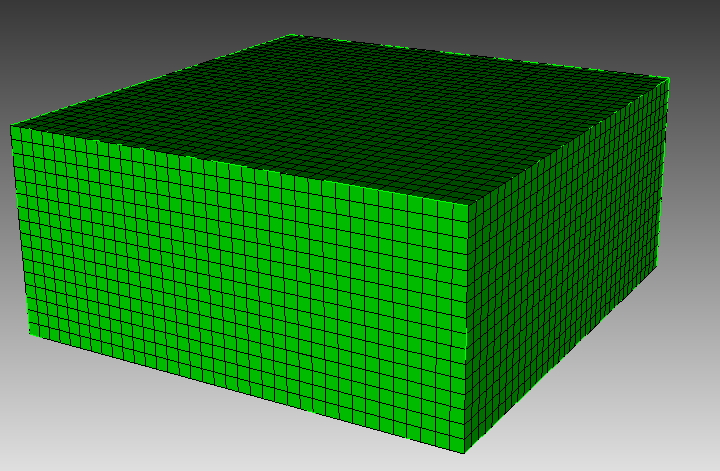
\includegraphics[width=0.45\textwidth]{figures/example-homogeneous}
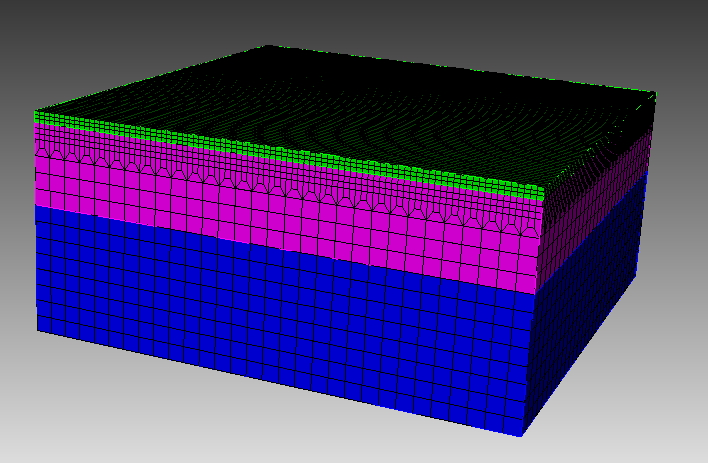
\includegraphics[width=0.45\textwidth]{figures/example-2layers} \\
 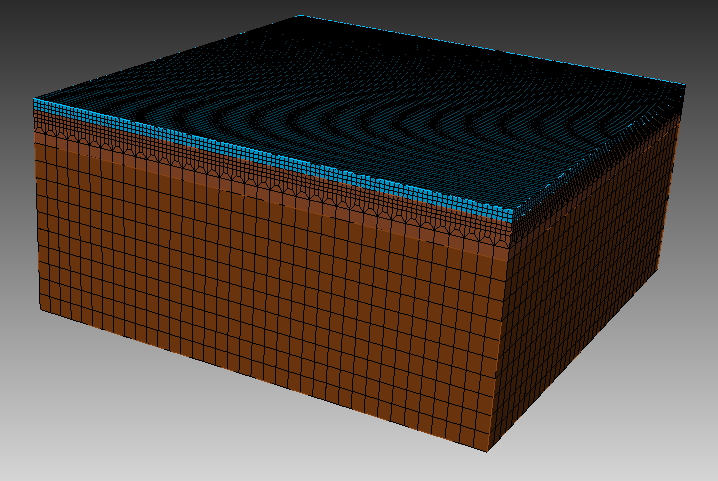
\includegraphics[width=0.45\textwidth]{figures/example-water} 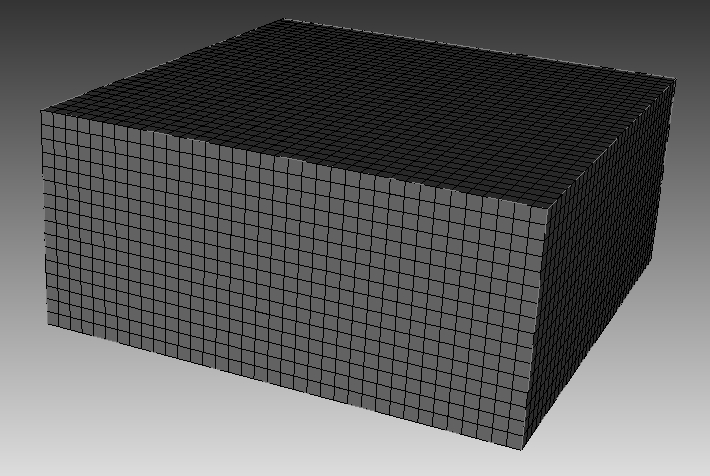
\includegraphics[width=0.45\textwidth]{figures/example-tomo}
\par\end{centering}

\caption{Screenshots of the CUBIT examples provided in subdirectory \texttt{examples/}:
homogeneous halfspace (top-left), layered halfspace (top-right), water
layered halfspace (bottom-left) and tomographic model (bottom-right).}


\label{fig:examples.cubit}
\end{figure}


In each example subdirectory you will find a \texttt{README} file,
which explains in a step-by-step tutorial the workflow for the example.
Please feel free to contribute your own example to this package by
contacting the CIG Computational Seismology Mailing List \urlwithparentheses{cig-seismo@geodynamics.org}.

In some cases, to re-create the meshes for the examples given, just type "claro ./create\_mesh.py" or similar 
from the command line ("claro" is the command to run CUBIT from the command line).

IMPORTANT note: in order to correctly set up GEOCUBIT and run the examples, please read the file called "examples/README";
in particular, please make sure you correctly set up the Python paths as indicated in that file.


\subsection{Exporting the Mesh with \texttt{run\_cubit2specfem3d.py} }

\label{subsec:Exporting-the-Mesh}

Once the geometric model volumes in CUBIT are meshed, you prepare
the model for exportation with the definition of material blocks and
boundary surfaces. Thus, prior to exporting the mesh, you need to
define blocks specifying the materials and absorbing boundaries in
CUBIT. This process could be done automatically using the script \texttt{run\_cubit2specfem3d.py}
if the mesh meets some conditions or manually, following the block
convention:
\begin{description}
\item [{material\_name}] Each material should have a specific block defined
by a unique name. The name convention of the material is to start
with either 'elastic' or 'acoustic'. It must be then followed by a
unique identifier, e.g. 'elastic 1', 'elastic 2', etc. The additional
attributes to the block define the material description.


For an elastic material:
\begin{description}
\item [{material\_id}] An integer value which is unique for this material.
\item [{Vp}] P-wave speed of the material (given in m/s).
\item [{Vs}] S-wave speed of the material (given in m/s).
\item [{rho}] density of the material (given in kg/m$^{3}$).
\item [{Q}] quality factor to use in case of a simulation with attenuation
turned on. It should be between 1 and 9000. In case no attenuation
information is available, it can be set to zero. Please note that
your Vp- and Vs-speeds are given for a reference frequency. To change
this reference frequency, you change the value of \texttt{ATTENUATION\_f0\_REFERENCE}
in the main constants file \texttt{constants.h} found in subdirectory
\texttt{src/shared/}.
\item [{anisotropic\_flag}] Flag describing the anisotropic model to use
in case an anisotropic simulation should be conducted. See the file
\texttt{model\_aniso.f90} in subdirectory \texttt{src/generate\_databases/}
for an implementation of the anisotropic models. In case no anisotropy
is available, it can be set to zero.
\end{description}

Note that this material block has to be defined using all the volumes
which belong to this elastic material. For volumes belonging to another,
different material, you will need to define a new material block.


For an acoustic material:
\begin{description}
\item [{material\_id}] An integer value which is unique for this material.
\item [{Vp}] P-wave speed of the material (given in m/s).
\item [{0}] S-wave speed of the material is ignored.
\item [{rho}] density of the material (given in kg/m$^{3}$).
\end{description}
\item [{face\_topo}] Block definition for the surface which defines the
free surface (which can have topography). The name of this block must
be 'face\_topo', the block has to be defined using all the surfaces
which constitute the complete free surface of the model.
\item [{face\_abs\_xmin}] Block definition for the faces on the absorbing
boundaries, one block for each surface with x=Xmin.
\item [{face\_abs\_xmax}] Block definition for the faces on the absorbing
boundaries, one block for each surface with x=Xmax.
\item [{face\_abs\_ymin}] Block definition for the faces on the absorbing
boundaries, one block for each surface with y=Ymin.
\item [{face\_abs\_ymax}] Block definition for the faces on the absorbing
boundaries, one block for each surface with y=Ymax.
\item [{face\_abs\_bottom}] Block definition for the faces on the absorbing
boundaries, one block for each surface with z=bottom.
\end{description}
\begin{figure}[htbp]
\noindent \begin{centering}
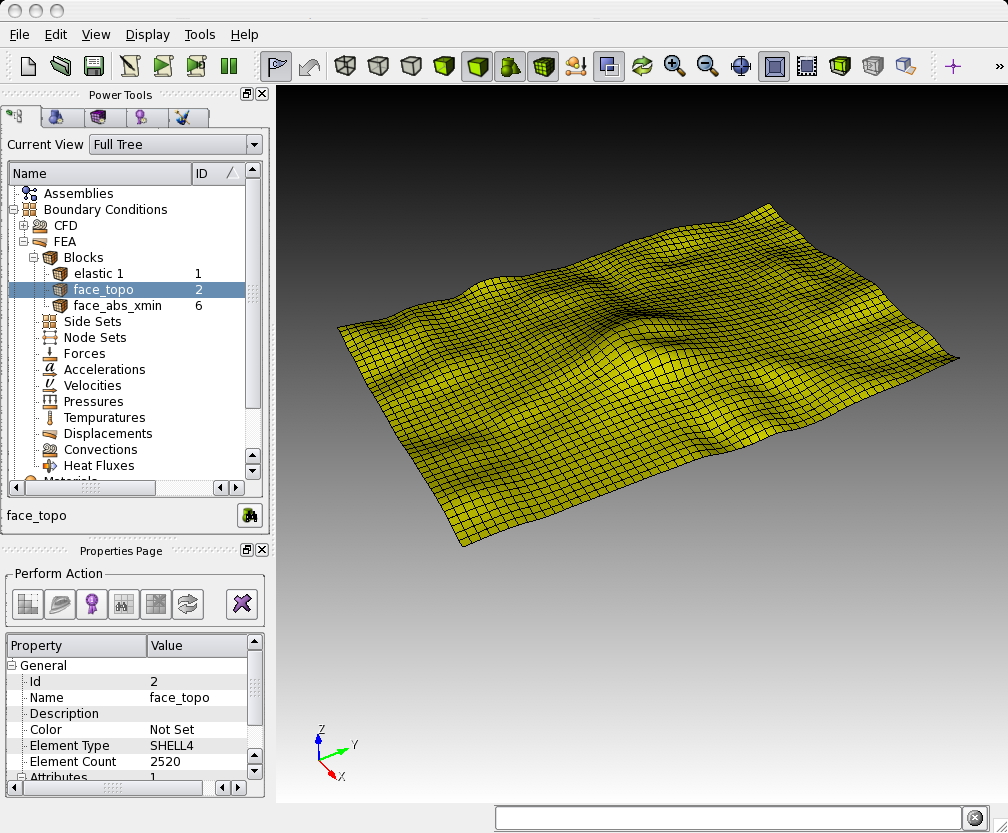
\includegraphics[width=0.45\textwidth]{figures/mount-surface} 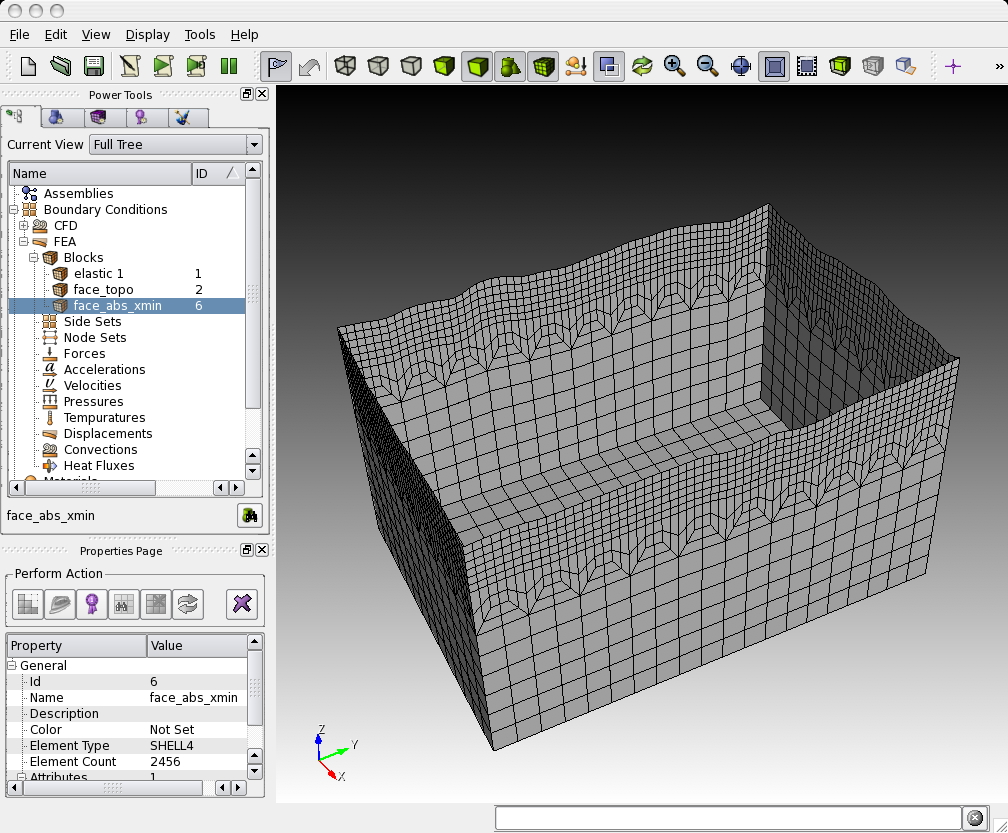
\includegraphics[width=0.45\textwidth]{figures/mount-abs}
\par\end{centering}

\caption{Example of the block definitions for the free surface 'face\_topo'
(left) and the absorbing boundaries, defined in a single block 'face\_abs\_xmin'
(right) in CUBIT.}


\label{fig:mount.abs}
\end{figure}


Optionally, instead of specifying for each surface at the boundaries
a single block like mentioned above, you can also specify a single
block for all boundary surfaces and name it as one of the absorbing
blocks above, e.g. 'face\_abs\_xmin'.

After the block definitions are done, you export the mesh using the
script \texttt{cubit2specfem3d.py} provided in each of the example
directories (linked to the common script \texttt{CUBIT\_GEOCUBIT/cubit2specfem3d.py}). If the export was successful, you should find the following
files in a subdirectory \texttt{MESH/}:
\begin{description}
\item [{absorbing\_cpml\_file}] \textbf{(only needed in case of C-PML absorbing
conditions)} Contains on the first line the total number of C-PML
spectral elements in the mesh, and then on the following line the
list of all these C-PML elements with two numbers per line: first
the spectral element number, and then a C-PML flag indicating to which
C-PML layer(s) that element belongs, according to the following convention:

\begin{itemize}
\item Flag = 1 : element belongs to a X CPML layer only (either in Xmin
or in Xmax),
\item Flag = 2 : element belongs to a Y CPML layer only (either in Ymin
or in Ymax),
\item Flag = 3 : element belongs to a Z CPML layer only (either in Zmin
or in Zmax),
\item Flag = 4 : element belongs to a X CPML layer and also to a Y CPML
layer,
\item Flag = 5 : element belongs to a X CPML layer and also to a Z CPML
layer,
\item Flag = 6 : element belongs to a Y CPML layer and also to a Z CPML
layer,
\item Flag = 7 : element belongs to a X, to a Y and to a Z CPML layer, i.e.,
it belongs to a CPML corner.
\end{itemize}

Note that it does not matter whether an element belongs to a Xmin
or to a Xmax CPML, the flag is the same in both cases; the same is
true for Ymin and Ymax, and also Zmin and Zmax.


When you have an existing CUBIT (or similar) mesh stored in SPECFEM3D
format, i.e., if you have existing \textquotedbl{}nodes\_coords\_file\textquotedbl{}
and \textquotedbl{}mesh\_file\textquotedbl{} files but do not know
how to assign CPML flags to them, we have created a small serial Fortran
program that will do that automatically for you, i.e., which will
create the \textquotedbl{}absorbing\_cpml\_file\textquotedbl{} for
you. That program is utils/CPML/convert\_external\_layers\_of\_a\_given\_mesh\_to\_CPML\_layers.f90,
and a small Makefile is provided in that directory (utils/CPML).


IMPORTANT: it is your responsibility to make sure that in the input
CUBIT (or similar) mesh that this code will read in SPECFEM3D format
from files \textquotedbl{}nodes\_coords\_file\textquotedbl{} and \textquotedbl{}mesh\_file\textquotedbl{}
you have created layers of elements that constitute a layer of constant
thickness aligned with the coordinate grid axes (X, Y and/or Z), so
that this code can assign CPML flags to them. This code does NOT check
that (because it cannot, in any easy way). The mesh inside these CPML
layers does not need to be structured nor regular, any non-structured
mesh is fine as long as it has flat PML inner and outer faces, parallel
to the axes, and thus of a constant thickness. The thickness can be
different for the X, Y and Z sides. But for X it must not vary, for
Y it must not vary, and for Z it must not vary. If you do not know
the exact thickness, you can use a slightly LARGER value in this code
(say 2\% to 5\% more) and this code will fix that and will adjust
it; never use a SMALLER value otherwise this code will miss some CPML
elements.


Note: in a future release we will remove the constraint of having
CPML layers aligned with the coordinate axes; we will allow for meshes
that are titled by any constant angle in the horizontal plane. However
this is not implemented yet.


Note: in the case of fluid-solid layers in contact, the fluid-solid
interface currently needs to be flat and horizontal inside the CPML
layer (i.e., bathymetry should become flat and horizontal when entering
the CPML); this (small) constraint will probably remain in the code
for a while because it makes fluid-solid matching inside the CPML
much easier.

\item [{materials\_file}] Contains the material associations for each element.
The format is:

\begin{lyxcode}
element\_ID~material\_ID
\end{lyxcode}

where \texttt{element\_ID} is the element identifier and \texttt{material\_ID}
is a unique identifier, positive (for materials taken from this list
of materials, i.e. for which each spectral element has constant material
properties taken from this list) or negative (for tomographic models,
i.e. for spectral element whose real velocities and density will be
assigned later by calling an external function to define model variations,
for instance in the case of tomographic models; in such a case, material
properties can vary inside each spectral element, i.e. be different
at each of its Gauss-Lobatto-Legendre grid points).

\item [{nummaterial\_velocity\_file}] Defines the material properties.

\begin{itemize}
\item For classical materials (i.e., spectral elements for which the velocity
and density model will not be assigned by calling an external function
to define for instance a tomographic model), the format is:

\begin{lyxcode}
domain\_ID~material\_ID~rho~vp~vs~Qkappa~Qmu~anisotropy\_flag
\end{lyxcode}

where \texttt{\textbf{domain\_ID}}\textbf{ is 1 for acoustic and 2
for elastic or viscoelastic materials,} \texttt{material\_ID} a unique
identifier, \texttt{rho} the density in $kg\, m^{-3}$, \texttt{vp}
the P-wave speed in $m\, s^{-1}$, \texttt{vs} the S-wave speed in
$m\, s^{-1}$, \texttt{Q} the quality factor and \texttt{anisotropy\_flag}
an identifier for anisotropic models. Note that the \texttt{Qkappa}
value is ignored by the code unless \texttt{FULL\_ATTENUATION\_SOLID}
is set. Note also that both \texttt{Qkappa} and \texttt{Qmu} are ignored
by the code unless \texttt{ATTENUATION} is set. If you want a model
with no \texttt{Qmu} attenuation, both set \texttt{ATTENUATION} to
\texttt{.false.} in the \texttt{Par\_file} and set \texttt{Qmu} to
9999 here. If you want a model with no \texttt{Qkappa} attenuation,
both set \texttt{FULL\_ATTENUATION\_SOLID} to \texttt{.false.} in
the \texttt{Par\_file} and set \texttt{Qkappa} to 9999 here. %%magnoni


\item For tomographic velocity models, please read Chapter \ref{cha:-Changing-the}
and Section \ref{sec:Using-tomographic} `Using external tomographic
Earth models' for further details.
\end{itemize}
\item [{nodes\_coords\_file}] Contains the point locations in Cartesian
coordinates of the mesh element corners.
\item [{mesh\_file}] Contains the mesh element connectivity. The hexahedral
elements can have 8 or 27 nodes.\\
 See picture doc/mesh\_numbering\_convention/numbering\_convention\_27\_nodes.jpg
to see\\
 in which (standard) order the points must be cited. In the case of
8 nodes, just include the first 8 points.
\item [{free\_or\_absorbing\_surface\_file\_zmax}] Contains the free surface
connectivity or \\
 the surface connectivity of the absorbing boundary surface at the
top (Zmax), \\
 depending on whether the top surface is defined as free or absorbing
(\texttt{STACEY\_INSTEAD\_OF\_FREE\_SURFACE} in \texttt{DATA/Par\_file}). \\
 You should put both the surface of acoustic regions and of elastic
regions in that file; that is, list all the element faces that constitute
the surface of the model in that file.
\item [{absorbing\_surface\_file\_xmax}] Contains the surface connectivity
of the absorbing boundary surface at Xmax \\
(also needed in the case of C-PML absorbing conditions, in order for
the code to be able to impose Dirichlet conditions on their outer
edge).
\item [{absorbing\_surface\_file\_xmin}] Contains the surface connectivity
of the absorbing boundary surface at Xmin \\
(also needed in the case of C-PML absorbing conditions, in order for
the code to be able to impose Dirichlet conditions on their outer
edge).
\item [{absorbing\_surface\_file\_ymax}] Contains the surface connectivity
of the absorbing boundary surface at Ymax \\
(also needed in the case of C-PML absorbing conditions, in order for
the code to be able to impose Dirichlet conditions on their outer
edge).
\item [{absorbing\_surface\_file\_ymin}] Contains the surface connectivity
of the absorbing boundary surface at Ymin \\
(also needed in the case of C-PML absorbing conditions, in order for
the code to be able to impose Dirichlet conditions on their outer
edge).
\item [{absorbing\_surface\_file\_bottom}] Contains the surface connectivity
of the absorbing boundary surface at the bottom (Zmin) \\
(also needed in the case of C-PML absorbing conditions, in order for
the code to be able to impose Dirichlet conditions on their outer
edge).
\end{description}
These mesh files are needed as input files for the partitioner \texttt{xdecompose\_mesh}
to load-balance the mesh. Please see the next section for further
details.

In directory "CUBIT\_GEOCUBIT" we provide a script that can help doing the above tasks of exporting a CUBIT mesh
to SPECFEM3D format automatically for you: "run\_cubit2specfem3d.py".
Just edit them to indicate the path to your local installation of CUBIT and also the name of the *.cub existing CUBIT mesh file
that you want to export to SPECFEM3D format. These scripts will do the conversion for you automatically except assigning material properties
to the different mesh layers. To do so, you will then need to edit the file 
called "nummaterial\_velocity\_file" that will have just been created and change it from the prototype created:

    0 1 vol1 --> syntax: \#material\_domain\_id \#material\_id \#rho \#vp \#vs \#Q\_kappa \#Q\_mu \#anisotropy
    0 2 vol2 --> syntax: \#material\_domain\_id \#material\_id \#rho \#vp \#vs \#Q\_kappa \#Q\_mu \#anisotropy

(where "vol1" and "vol2" here represent the volume labels that you have set while creating the mesh in CUBIT)
to for instance

    2 1 1500 2300 1800 9999.0 9999.0 0
    2 2 1600 2500 20000 9999.0 9999.0 0


\subsubsection*{Checking the mesh quality}

The quality of the mesh may be inspected more precisely based upon
the serial code in the file \texttt{check\_mesh\_quality\_}~\\
 \texttt{CUBIT\_Abaqus.f90} located in the directory \texttt{src/check\_mesh\_quality\_CUBIT\_Abaqus/}.
Running this code is optional because no information needed by the
solver is generated.

Prior to running and compiling this code, you have to export your
mesh in CUBIT to an ABAQUS (.inp) format. For example, export mesh
block IDs belonging to volumes in order to check the quality of the
hexahedral elements. You also have to determine a number of parameters
of your mesh, such as the number of nodes and number of elements and
modify the header of the \texttt{check\_mesh\_quality\_CUBIT\_Abaqus.f90}
source file. Then, in the main directory, type
\begin{lyxcode}
{\small make~xcheck\_mesh\_quality\_CUBIT\_Abaqus}{\small \par}
\end{lyxcode}
and use
\begin{lyxcode}
{\small ./bin/xcheck\_mesh\_quality\_CUBIT\_Abaqus}{\small \par}
\end{lyxcode}
to generate an %not supported: AVS output file (\texttt{\small AVS\_meshquality.inp} in AVS UCD format) or
OpenDX output file (\texttt{\small DX\_mesh\_quality.dx}{\small )
that can be used to investigate mesh quality, e.g. skewness of elements,
and a Gnuplot histogram (}\texttt{\small mesh\_quality\_histogram.txt}{\small )
that can be plotted with gnuplot (type `}\texttt{\small gnuplot plot\_mesh\_quality\_histogram.gnu}{\small ').
The histogram is also printed to the screen. Analyze that skewness
histogram of mesh elements to make sure no element has a skewness
above approximately 0.75, otherwise the mesh is of poor quality (and
if even a single element has a skewness value above 0.80, then you
must definitely improve the mesh). If you want to start designing
your own meshes, this tool is useful for viewing your creations. You
are striving for meshes with elements with `cube-like' dimensions,
e.g., the mesh should contain no very elongated or skewed elements.}{\small \par}


\subsection{Partitioning the Mesh with \texttt{xdecompose\_mesh}}

The SPECFEM3D Cartesian software package performs large scale simulations
in a parallel 'Single Process Multiple Data' way. The spectral-element
mesh created with CUBIT needs to be distributed on the processors.
This partitioning is executed once and for all prior to the execution
of the solver so it is referred to as a static mapping.

An efficient partitioning is important because it leverages the overall
running time of the application. It amounts to balance the number
of elements in each slice while minimizing the communication costs
resulting from the placement of adjacent elements on different processors.
\texttt{decompose\_mesh} depends on the SCOTCH library \citep{PeRo96},
which provides efficent static mapping, graph and mesh partitioning
routines. SCOTCH is a free software package developed by Fran�ois
Pellegrini et al. from LaBRI and INRIA in Bordeaux, France, downloadable
from the web page \url{https://gforge.inria.fr/projects/scotch/}.
\\


In most cases, the configuration with \texttt{./configure~FC=ifort}
should be sufficient. During the configuration process, the script
tries to find existing SCOTCH installations. In case your system has
no pre-existing SCOTCH installation, we provide the source code of
SCOTCH, which is released open source under the French CeCILL-C version
1 license, in directory \texttt{src/decompose\_mesh/scotch\_5.1.12b}.
This version gets bundled with the compilation of the SPECFEM3D Cartesian
package if no libraries could have been found. If this automatic compilation
of the SCOTCH libraries fails, please refer to file INSTALL.txt in
that directory to see further details how to compile it on your system.
In case you want to use a pre-existing installation, make sure you
have correctly specified the path of the SCOTCH library when using
the option \texttt{-{}-with-scotch-dir} with the \texttt{./configure}
script. In the future you should be able to find more recent versions
at \url{http://www.labri.fr/perso/pelegrin/scotch/scotch_en.html}
. \\


\begin{figure}[htbp]
\noindent \begin{centering}
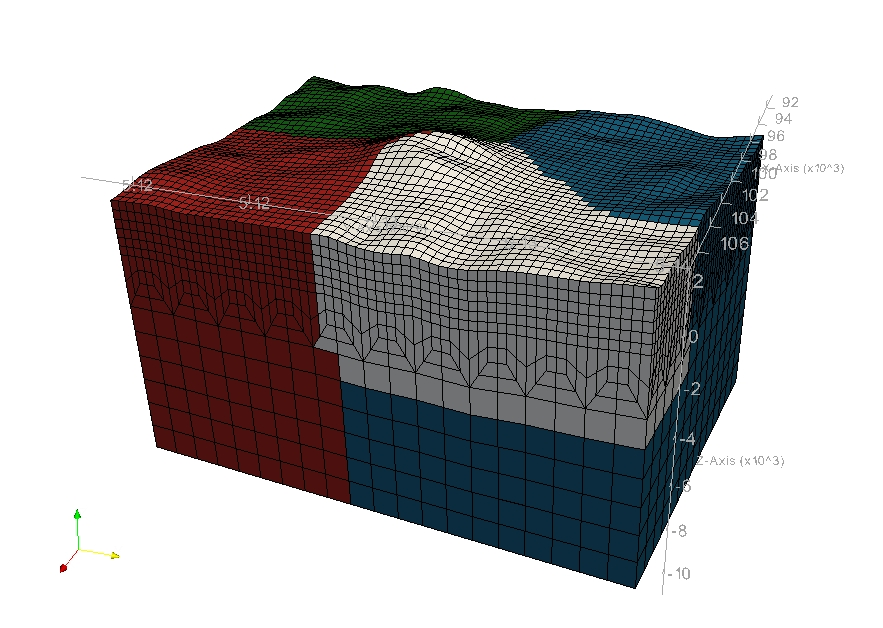
\includegraphics[width=0.45\textwidth]{figures/mount-partitions}
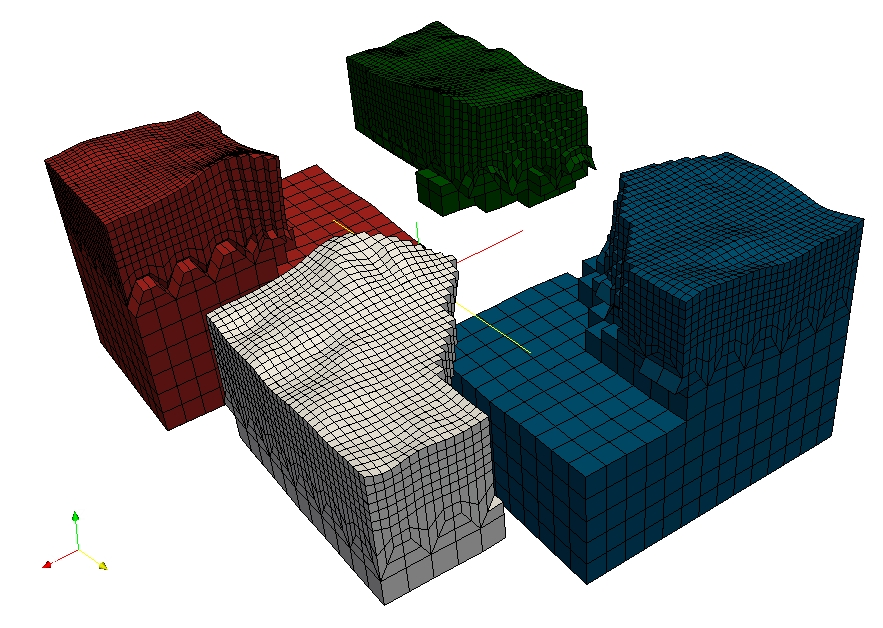
\includegraphics[width=0.45\textwidth]{figures/mount-partitions2}
\par\end{centering}

\caption{Example of a mesh partitioning onto four cores. Each single core partition
is colored differently. The executable \texttt{xdecompose\_mesh} can
equally distribute the mesh on any arbitrary number of cores. Domain
decomposition is explained in detail in \citet{MaKoBlLe08}, and excellent
scaling up to 150,000 processor cores in shown for instance in \citet{CaKoLaTiMiLeSnTr08,KoLaMi08a,MaKoBlLe08,KoErGoMi10,Kom11}.}


\label{fig:mount.partitions}
\end{figure}


When you are ready to compile, in the main directory type
\begin{lyxcode}
{\small make~xdecompose\_mesh}{\small \par}
\end{lyxcode}
If all paths and flags have been set correctly, the executable \texttt{bin/xdecompose\_mesh}
should be produced.

The partitioning is done in serial for now (in the next release we
will provide a parallel version of that code). It needs to be run in the \texttt{bin/} directory because it expects the \texttt{../DATA/Par\_file}. The synopsis is:
\begin{lyxcode}
./xdecompose\_mesh~nparts~input\_directory~output\_directory
\end{lyxcode}
where
\begin{itemize}
\item \texttt{nparts} is the number of partitions, i.e., the number of cores
for the parallel simulations,
\item \texttt{input\_directory} is the directory which holds all the files
generated by the Python script \texttt{cubit2specfem3d.py} explained
in the previous Section~\ref{subsec:Exporting-the-Mesh}, e.g. \texttt{MESH/},
and
\item \texttt{output\_directory} is the directory for the output of this
partitioner which stores ACII-format files named like \texttt{proc{*}{*}{*}{*}{*}{*}\_Database}
for each partition. These files will be needed for creating the distributed
databases, and have to reside in the directory \texttt{LOCAL\_PATH}
specified in the main \texttt{Par\_file}, e.g. in directory \texttt{OUTPUT\_FILES/DATABASES\_MPI}.
Please see Chapter~\ref{cha:Creating-Distributed-Databases} for
further details.
\end{itemize}
Note that all the files generated by the Python script \texttt{cubit2specfem3d.py}
must be placed in the \texttt{input\_directory} folder before running
the program.


\section{\label{cha:Running-the-Mesher-Meshfem3D}Meshing with \texttt{xmeshfem3D}}

In case you successfully ran the configuration script, you are also
ready to compile the internal mesher. This is an alternative to CUBIT
for the mesh generation of relatively simple geological models. The
mesher is no longer dedicated to Southern California and more flexiblity
is provided in this version of the package.

\begin{figure}[htbp]
\noindent \begin{centering}
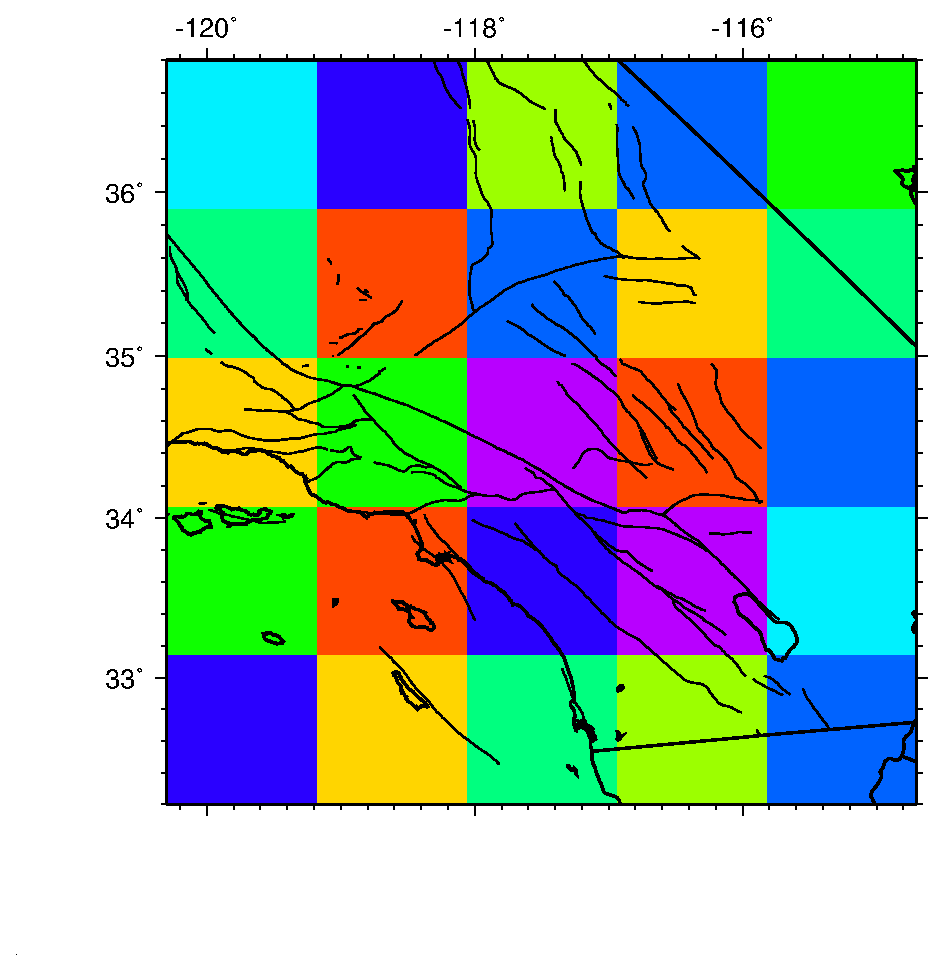
\includegraphics[scale=0.5]{figures/socal_map_mpi}
\par\end{centering}

\caption{\label{fig:For-parallel-computing}For parallel computing purposes,
the model block is subdivided in $\nprocxi\times\nproceta$ slices
of elements. In this example we use $5^{2}=25$ processors. }
\end{figure}


In the main directory, type
\begin{lyxcode}
{\small make~xmeshfem3D}{\small \par}
\end{lyxcode}
If all paths and flags have been set correctly, the mesher should
now compile and produce the executable \texttt{bin/xmeshfem3D}. Please
note that \texttt{xmeshfem3D} must be called directly from the \texttt{bin/}
directory, as most of the binaries of the package.

Input for the mesh generation program is provided through the parameter
file \texttt{Mesh\_Par\_file}, which resides in the subdirectory \texttt{DATA/meshfem3D\_files/}.
Before running the mesher, a number of parameters need to be set in
the \texttt{Mesh\_Par\_file}. This requires a basic understanding
of how the SEM is implemented, and we encourage you to read \citet{KoVi98,KoTr99}
and \citet{KoLiTrSuStSh04}.

The mesher and the solver use UTM coordinates internally, therefore
you need to define the zone number for the UTM projection (e.g., zone
11 for Los Angeles). Use decimal values for latitude and longitude
(no minutes/seconds). These values are approximate; the mesher will
round them off to define a square mesh in UTM coordinates. When running
benchmarks on rectangular models, turn the UTM projection off by using
the flag \texttt{\small SUPPRESS\_UTM\_PROJECTION}{\small , in which
case all `longitude' parameters simply refer to the $x$~axis, and
all `latitude' parameters simply refer to the $y$~axis. To run the
mesher for a global simulation, the following parameters need to be
set in the }\texttt{\small Mesh\_Par\_file}{\small :}{\small \par}
\begin{description}
\item [{\texttt{LATITUDE\_MIN}}] Minimum latitude in the block (negative
for South).
\item [{\texttt{LATITUDE\_MAX}}] Maximum latitude in the block.
\item [{\texttt{LONGITUDE\_MIN}}] Minimum longitude in the block (negative
for West).
\item [{\texttt{LONGITUDE\_MAX}}] Maximum longitude in the block.
\item [{\texttt{DEPTH\_BLOCK\_KM}}] Depth of bottom of mesh in kilometers.
\item [{\texttt{\noun{UTM\_PROJECTION\_ZONE}}}] UTM projection zone in
which your model resides, only valid when \texttt{SUPPRESS\_UTM\_}~\\
 \texttt{PROJECTION} is \texttt{.false.}.
\item [{\texttt{SUPPRESS\_UTM\_PROJECTION}}] set to be \texttt{.false.}
when your model range is specified in geographical coordinates, and
needs to be \texttt{.true.} when your model is specified in Cartesian
coordinates. \noun{UTM projection zone in which your simulation region
resides.}
\item [{\texttt{INTERFACES\_FILE }}] File which contains the description
of the topography and of the interfaces between the different layers
of the model, if any. The number of spectral elements in the vertical
direction within each layer is also defined in this file.
\item [{$\nexxi$}] The number of spectral elements along one side of the
block. This number \textit{must} be 8~$\times$~a multiple of $\nprocxi$
defined below. Based upon benchmarks against semi-analytical discrete
wavenumber synthetic seismograms \citep{KoLiTrSuStSh04}, determined
that a $\nexxi=288$ run is accurate to a shortest period of roughly
2~s. Therefore, since accuracy is determined by the number of grid
points per shortest wavelength, for any particular value of $\nexxi$
the simulation will be accurate to a shortest period determined by
\begin{equation}
\mbox{shortest period (s)}=(288/\nexxi)\times2.\label{eq:shortest_period}
\end{equation}
 The number of grid points in each orthogonal direction of the reference
element, i.e., the number of Gauss-Lobatto-Legendre points, is determined
by \texttt{NGLLX} in the \texttt{constants.h} file. We generally use
$\mbox{\texttt{NGLLX\/}}=5$, for a total of $5^{3}=125$ points per
elements. We suggest not to change this value.
\item [{$\nexeta$}] The number of spectral elements along the other side
of the block. This number \textit{must} be 8~$\times$~a multiple
of $\nproceta$ defined below.
\item [{$\nprocxi$}] The number of processors or slices along one side
of the block (see Figure~\ref{fig:For-parallel-computing}); we must
have $\nexxi=8\times c\times\nprocxi$, where $c\ge1$ is a positive
integer.
\item [{$\nproceta$}] The number of processors or slices along the other
side of the block; we must have $\nexeta=8\times c\times\nproceta$,
where $c\ge1$ is a positive integer.
\item [{\texttt{USE\_REGULAR\_MESH}}] set to be \texttt{.true.} if you
want a perfectly regular mesh or \texttt{.false.} if you want to add
doubling horizontal layers to coarsen the mesh. In this case, you
also need to provide additional information by setting up the next
three parameters.
\item [{\texttt{NDOUBLINGS}}] The number of horizontal doubling layers.
Must be set to \texttt{1} or \texttt{2} if \texttt{USE\_REGULAR\_MESH}
is set to \texttt{.true.}.
\item [{\texttt{NZ\_DOUBLING\_1}}] The position of the first doubling layer
(only interpreted if \texttt{USE\_REGULAR\_MESH} is set to \texttt{.true.}).
\item [{\texttt{NZ\_DOUBLING\_2}}] The position of the second doubling
layer (only interpreted if \texttt{USE\_REGULAR\_MESH} is set to \texttt{.true.}
and if \texttt{NDOUBLINGS} is set to \texttt{2}).
\item [{\texttt{CREATE\_ABAQUS\_FILES}}] Set this flag to \texttt{.true.}
to save Abaqus FEA \urlwithparentheses{www.simulia.com} mesh files
for subsequent viewing. Turning the flag on generates files in the
\texttt{LOCAL\_PATH} directory. See Section~\ref{sec:Mesh-graphics}
for a discussion of mesh viewing features.
\item [{\texttt{CREATE\_DX\_FILES}}] Set this flag to \texttt{.true.} to
save OpenDX \urlwithparentheses{www.opendx.org} mesh files for subsequent
viewing.
\item [{\texttt{LOCAL\_PATH}}] Directory in which the partitions generated
by the mesher will be written. Generally one uses a directory on the
local disk of the compute nodes, although on some machines these partitions
are written on a parallel (global) file system (see also the earlier
discussion of the \texttt{LOCAL\_PATH\_IS\_ALSO\_GLOBAL} flag in Chapter~\ref{cha:Getting-Started}).
The mesher generates the necessary partitions in parallel, one set
for each of the $\nprocxi\times\nproceta$ slices that constitutes
the mesh (see Figure~\ref{fig:For-parallel-computing}). After the
mesher finishes, you can log in to one of the compute nodes and view
the contents of the \texttt{LOCAL\_PATH} directory to see the files
generated by the mesher. These files will be needed for creating the
distributed databases, and have to reside in the directory \texttt{LOCAL\_PATH}
specified in the main \texttt{Par\_file}, e.g. in directory \texttt{OUTPUT\_FILES/DATABASES\_MPI}.
Please see Chapter~\ref{cha:Creating-Distributed-Databases} for
further details.
\item [{\texttt{NMATERIALS}}] The number of different materials in your
model. In the following lines, each material needs to be defined as
:

\begin{lyxcode}
material\_ID~rho~vp~vs~Q~anisotropy\_flag~domain\_ID
\end{lyxcode}

where
\begin{itemize}
\item \texttt{Q} : quality factor (0=no attenuation)
\item \texttt{anisotropy\_flag} : 0=no anisotropy / 1,2,.. check with implementation
in \texttt{aniso\_model.f90}
\item \texttt{domain\_id} : 1=acoustic / 2=elastic
\end{itemize}
\item [{\texttt{NREGIONS}}] The number of regions in the mesh. In the following
lines, because the mesh is regular or 'almost regular', each region
is defined as :

\begin{lyxcode}
NEX\_XI\_BEGIN~NEX\_XI\_END~NEX\_ETA\_BEGIN~NEX\_ETA\_END~NZ\_BEGIN~NZ\_END~material\_ID
\end{lyxcode}
\end{description}
The \texttt{INTERFACES\_FILE} parameter of \texttt{Mesh\_Par\_File}
defines the file which contains the settings of the topography grid
and of the interfaces grids. Topography is defined as a set of elevation
values on a regular 2D grid. It is also possible to define interfaces
between the layers of the model in the same way. The file needs to
define several parameters:
\begin{itemize}
\item The number of interfaces, including the topography. This needs to
be set at the first line. Then, from the bottom to the top of the
model, you need to define the grids with:
\item \texttt{SUPPRESS\_UTM\_PROJECTION} flag as described previously,
\item number of points along $x$ and $y$ direction (NXI and NETA),
\item minimal $x$ and $y$ coordinates (LONG\_MIN and LAT\_MIN),
\item spacing between points along $x$ and $y$ (SPACING\_XI and SPACING\_ETA)
and
\item the name of the file which contains the elevation values (in $y$.$x$
increasing order).
\end{itemize}
At the end of this file, you simply need to set the number of spectral
elements in the vertical direction for each layer. We provide a few
models in the {\texttt{examples/}} directory. \\


Finally, depending on your system, you might need to provide a file
that tells MPI what compute nodes to use for the simulations. The
file must have a number of entries (one entry per line) at least equal
to the number of processors needed for the run. A sample file is provided
in the file \texttt{mymachines}. This file is not used by the mesher
or solver, but is required by the \texttt{go\_mesher} and \texttt{go\_solver}
default job submission scripts. See Chapter~\ref{cha:Scheduler}
for information about running the code on a system with a scheduler,
e.g., LSF.

Now that you have set the appropriate parameters in the \texttt{Mesh\_Par\_file}
and have compiled the mesher, you are ready to launch it! This is
most easily accomplished based upon the \texttt{go\_mesher} script.
When you run on a PC cluster, the script assumes that the nodes are
named n001, n002, etc. If this is not the case, change the \texttt{tr
-d `n'} line in the script. You may also need to edit the last command
at the end of the script that invokes the \texttt{mpirun} command.
See Chapter~\ref{cha:Scheduler} for information about running the
code on a system with a scheduler, e.g., LSF.

Mesher output is provided in the \texttt{OUTPUT\_FILES} directory
in \texttt{output\_mesher.txt}; this file provides lots of details
about the mesh that was generated. Please note that the mesher suggests
a time step \texttt{DT} to run the solver with. The mesher output
file also contains a table about the quality of the mesh to indicate
possible problems with the distortions of elements. Alternatively,
output can be directed to the screen instead by uncommenting a line
in \texttt{constants.h}:
\begin{lyxcode}
!~uncomment~this~to~write~messages~to~the~screen~

!~integer,~parameter~::~IMAIN~=~ISTANDARD\_OUTPUT
\end{lyxcode}
To control the quality of the mesh, check the standard output (either
on the screen or in the \texttt{OUTPUT\_FILES} directory in \texttt{output\_mesher.txt})
and analyze the skewness histogram of mesh elements to make sure no
element has a skewness above approximately 0.75, otherwise the mesh
is of poor quality (and if even a single element has a skewness value
above 0.80, then you must definitely improve the mesh). To draw the
skewness histogram on the screen, type \texttt{gnuplot plot\_mesh\_quality\_histogram.gnu}.


\chapter{\label{cha:Creating-Distributed-Databases}Creating the Distributed
Databases}

After using \texttt{xmeshfem3D} or \texttt{xdecompose\_mesh}, the
next step in the workflow is to compile \texttt{xgenerate\_}~\\
 \texttt{databases}. This program is going to create all the missing
information needed by the SEM solver.

\begin{figure}[htbp]
\noindent \begin{centering}
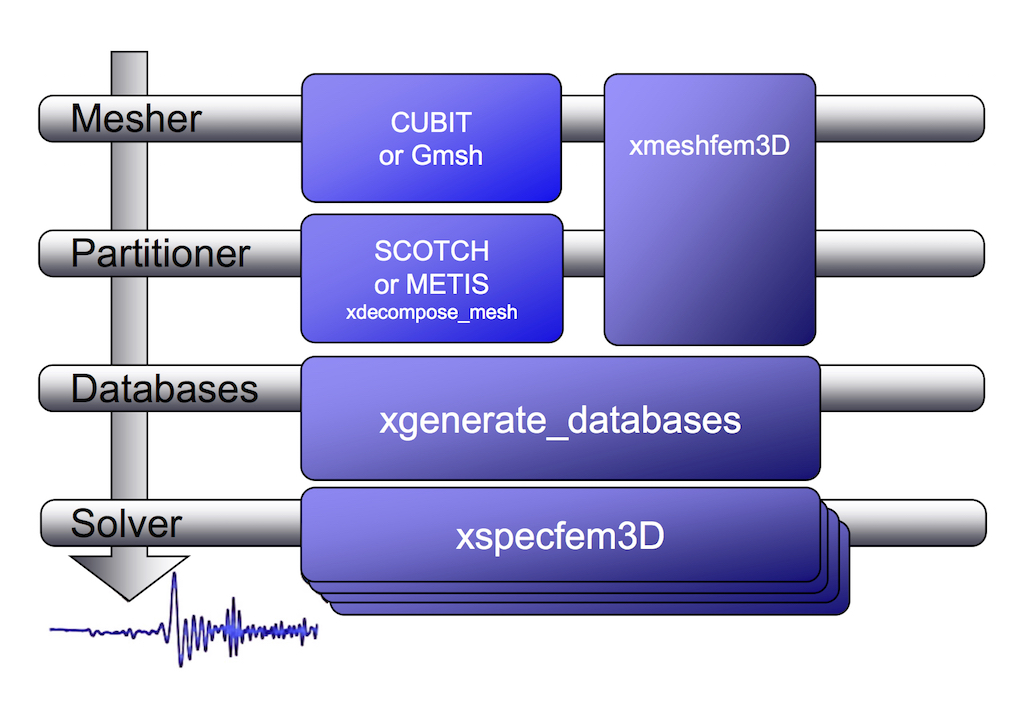
\includegraphics[width=0.6\textwidth]{figures/workflow}
\par\end{centering}

\caption{Schematic workflow for a SPECFEM3D Cartesian simulation. The executable
\texttt{xgenerate\_databases} creates the GLL mesh points and assigns
specific model parameters.}


\label{fig:workflow.databases}
\end{figure}


In the main directory, type
\begin{lyxcode}
{\small make~xgenerate\_databases}{\small \par}
\end{lyxcode}
Input for the program is provided through the main parameter file
\texttt{Par\_file}, which resides in the subdirectory \texttt{DATA}.
Please note that \texttt{xgenerate\_databases} must be called directly
from the \texttt{bin/} directory, as most of the binaries of the package.


\section{\label{cha:Main-Parameter}Main parameter file \texttt{Par\_file}}

Before running \texttt{xgenerate\_databases}, a number of parameters
need to be set in the main parameter \texttt{Par\_file} located in
the subdirectory \texttt{DATA}:
\begin{description}
\item [{\texttt{SIMULATION\_TYPE}}] is set to 1 for forward simulations,
2 for adjoint simulations (see Section \ref{sec:Adjoint-simulation-finite})
and 3 for kernel simulations (see Section \ref{sec:Finite-Frequency-Kernels}).
\item [{\texttt{SAVE\_FORWARD}}] is only set to \texttt{.true.} for a forward
simulation with the last frame of the simulation saved, as part of
the finite-frequency kernel calculations (see Section \ref{sec:Finite-Frequency-Kernels}).
For a regular forward simulation, leave \texttt{SIMULATION\_TYPE}
and \texttt{SAVE\_FORWARD} at their default values.
\item [{\texttt{\noun{UTM\_PROJECTION\_ZONE}}}] UTM projection zone in
which your model resides, only valid when \texttt{SUPPRESS\_UTM\_}~\\
 \texttt{PROJECTION} is \texttt{.false.}.
\item [{\texttt{SUPPRESS\_UTM\_PROJECTION}}] set to be \texttt{.false.}
when your model range is specified in the geographical coordinates,
and needs to be \texttt{.true.} when your model is specified in a
cartesian coordinates. \noun{UTM projection zone in which your simulation
region resides.}
\item [{\texttt{NPROC}}] The number of MPI processors, each one is assigned
one slice of the whole mesh.
\item [{\texttt{NSTEP}}] The number of time steps of the simulation. This
controls the length of the numerical simulation, i.e., twice the number
of time steps requires twice as much CPU time. This feature is not
used at the time of generating the distributed databases but is required
for the solver, i.e., you may change this parameter after running
\texttt{xgenerate\_databases}.
\item [{\texttt{DT}}] The length of each time step in seconds. This feature
is not used at the time of generating the distributed databases but
is required for the solver. Please see also Section~\ref{sec:Choosing-the-Time-Step}
for further details.
\item [{\texttt{NGNOD}}] The number of nodes for 2D and 3D shape functions
for hexahedra. We use either 8-node mesh elements (bricks) or 27-node
elements. If you use the internal mesher, the only option is 8-node
bricks (27-node elements are not supported). \texttt{CUBIT} does not
support HEX27 elements either (it can generate them, but they are
flat, i.e. identical to HEX8). To generate HEX27 elements with curvature
properly taken into account, you can use \texttt{Gmsh} \url{http://geuz.org/gmsh/}
\item [{\texttt{MODEL}}] Must be set to one of the following:

\begin{description}
\item [{\textmd{Models defined by mesh parameters:}}] ~

\begin{description}
\item [{\texttt{default}}] Uses model parameters as defined by meshing
procedures described in the previous Chapter~\ref{cha:Mesh-Generation}.
\end{description}

\item [{\textmd{1D~models~with~real~structure:}}] ~

\begin{description}
\item [{\texttt{1D\_prem}}] Isotropic version of the spherically symmetric
Preliminary Reference Earth Model (PREM) \citep{DzAn81}.
\item [{\texttt{1D\_socal}}] A standard isotropic 1D model for Southern
California.
\item [{\texttt{1D\_cascadia}}] Isotropic 1D profile for the Cascadia region.
\end{description}

\item [{\textmd{Fully~3D~models:}}] ~

\begin{description}
\item [{\texttt{aniso}}] For a user-specified fully anisotropic model.
Parameters are set up in routines located in file \texttt{model\_aniso.f90}
in directory \texttt{src/generate\_databases/}. See Chapter~\ref{cha:-Changing-the}
for a discussion on how to specify your own 3D model.

\item [{\texttt{external}}] For a user-specified isotropic model which
uses externally defined model parameters. Uses external model definitions
set up in routines located in file \texttt{model\_external\_values.f90}
in directory \texttt{src/generate\_databases/}. Please modify these
generic template routines to use your own model definitions.
\item [{\texttt{gll}}] For a user-specified isotropic model which uses
external binary files for $v_{p}$, $v_{s}$ and $\rho$. Binary files
are given in the same format as when outputted by the \texttt{xgenerate\_databases}
executable when using option \texttt{SAVE\_MESH\_FILES}. These binary
files define the model parameters on all GLL points which can be used
for iterative inversion procedures.
\item [{\texttt{salton\_trough}}] A 3D $V_{p}$ model for Southern California.
Users must provide the corresponding data file \texttt{regrid3\_vel\_p.bin}
in directory \texttt{DATA/st\_3D\_block\_harvard/}.
\item [{\texttt{tomo}}] For a user-specified 3D isotropic model which uses
a tomographic model file \texttt{tomographic\_model.xyz} in directory
\texttt{DATA}. See Section \ref{sec:Using-tomographic}, for a discussion
on how to specify your own 3D tomographic model.
\end{description}
\end{description}
\item [{\texttt{APPROXIMATE\_OCEAN\_LOAD}}] Set to \texttt{.true.} if the
effect of the oceans on seismic wave propagation should be incorporated
based upon the (rough) approximate treatment discussed in \citet{KoTr02b}.
This feature is inexpensive from a numerical perspective, both in
terms of memory requirements and CPU time. This approximation is accurate
at periods of roughly 20~s and longer. At shorter periods the effect
of water phases/reverberations is not taken into account, even when
the flag is on. If you want to model the effect of a fluid-solid model
at short periods, then set this flag to \texttt{.false.} and mesh
the fluid layer explicitly in your mesher, so that it is computed
accurately and without this approximation.
\item [{\texttt{TOPOGRAPHY}}] This feature is only effective if \texttt{APPROXIMATE\_OCEAN\_LOAD}
is set to \texttt{.true.}. Set to \texttt{.true.} if topography and
bathymetry should be read in based upon the topography file specified
in the main constants file \texttt{constants.h} found in subdirectory
\texttt{src/shared/} to evaluate elevations. If not set, elevations
will be read from the numerical mesh.
\item [{\texttt{ATTENUATION}}] Set to \texttt{.true.} if attenuation should
be incorporated. Turning this feature on increases the memory requirements
significantly (roughly by a factor of~1.5), and is numerically fairly
expensive. See \citet{KoTr99,KoTr02a} for a discussion on the implementation
of attenuation based upon standard linear solids. Please note that
the Vp- and Vs-velocities of your model are given for a reference
frequency. To change this reference frequency, you change the value
of \texttt{ATTENUATION\_f0\_REFERENCE} in the main constants file
\texttt{constants.h} found in subdirectory \texttt{src/shared/}.
\item [{\texttt{FULL\_ATTENUATION\_SOLID}}] Set to \texttt{.true.} to add
$Q_{\kappa}$ attenuation to the simulations in addition to $Q_{\mu}$
attenuation when the \texttt{ATTENUATION} flag above is on. Should
be off in almost all cases for seismic wave propagation, since $Q_{\kappa}$
is almost always negligible in Earth models. However, this parameter
can be useful for instance for ocean acoustics simulations, when $Q_{\kappa}$
is not negligible in the solid layer at the sea bottom.
\item [{\texttt{ANISOTROPY}}] Set to \texttt{.true.} if you want to use
an anisotropy model. Please see the file \texttt{model\_aniso.f90}
in subdirectory \texttt{src/generate\_databases/} for the current
implementation of anisotropic models.
\item [{\texttt{TOMOGRAPHY\_PATH}}] Directory in which the tomography files
are stored for using external tomographic Earth models (please read
Chapter \ref{cha:-Changing-the} and Section \ref{sec:Using-tomographic}
`Using external tomographic Earth models' for further details.).
\item [{\texttt{USE\_OLSEN\_ATTENUATION}}] Set to \texttt{.true.} if you
want to use the attenuation model that scaled from the S-wave speed
model using Olsen's empirical relation (see \citet{OlDaBr03}).
\item [{\texttt{OLSEN\_ATTENUATION\_RATIO}}] Determines the Olsen's constant
in Olsen's empirical relation (see \citet{OlDaBr03}).
\item [{\texttt{PML\_CONDITIONS}}] Set to \texttt{.true.} to turn on C-PML
boundary conditions for a regional simulation. Both fluids and elastic
solids are supported. Note that xmeshfem3d generated meshes do not support C-PML yet.
\item [{\texttt{PML\_INSTEAD\_OF\_FREE\_SURFACE}}] Set to \texttt{.true.}
to turn on C-PML boundary conditions on the top surface instead of
the usual free surface.
\item [{\texttt{f0\_FOR\_PML}}] Determines the dominant frequency that
will be used in the calculation of PML damping profiles; this should
be set to the same (or similar) dominant frequency as that of the
source that you will use in your simulation. If you plan to use a
Dirac source, then use the dominant frequency of the source wavelet
with which you plan to convolve your seismograms later on in post-processing.
\item [{\texttt{STACEY\_ABSORBING\_CONDITIONS}}] Set to \texttt{.true.}
to turn on Clayton-Enquist absorbing boundary conditions (see \citet{KoTr99}).
In almost all cases it is much better to use CPML absorbing layers
(see the options above) and leave this flag to \texttt{.false.}.
\item [{\texttt{STACEY\_INSTEAD\_OF\_FREE\_SURFACE}}] Set to \texttt{.true.}
to turn on absorbing boundary conditions on the top surface which
by default constitutes a free surface of the model.
\item [{\texttt{CREATE\_SHAKEMAP}}] Set this flag to \texttt{.true.} to
create a ShakeMap\textregistered{}, i.e., a peak ground velocity map
of the maximum absolute value of the two horizontal components of
the velocity vector.
\item [{\texttt{MOVIE\_SURFACE}}] Set to \texttt{.false.}, unless you want
to create a movie of seismic wave propagation on the Earth's surface.
Turning this option on generates large output files. See Section~\ref{sec:Movies}
for a discussion on the generation of movies. This feature is only
relevant for the solver.
\item [{\texttt{MOVIE\_TYPE}}] Set this flag to 1 to show the top surface
(tomography + oceans) only, to 2 to show all external faces of the
mesh (i.e. topography + vertical edges + bottom) in shakemaps and
surface movies.
\item [{\texttt{MOVIE\_VOLUME}}] Set to \texttt{.false.}, unless you want
to create a movie of seismic wave propagation in the Earth's interior.
Turning this option on generates huge output files. See Section~\ref{sec:Movies}
for a discussion on the generation of movies. This feature is only
relevant for the solver.
\item [{\texttt{SAVE\_DISPLACEMENT}}] Set this flag to \texttt{.true.}
if you want to save the displacement instead of velocity for the movie
frames.
\item [{\texttt{USE\_HIGHRES\_FOR\_MOVIES}}] Set this flag to \texttt{.true.}
if you want to save the values at all the NGLL grid points for the
movie frames.
\item [{\texttt{NTSTEP\_BETWEEN\_FRAMES}}] Determines the number of timesteps
between movie frames. Typically you want to save a snapshot every
100 timesteps. The smaller you make this number the more output will
be generated! See Section~\ref{sec:Movies} for a discussion on the
generation of movies. This feature is only relevant for the solver.
\item [{\texttt{HDUR\_MOVIE}}] Determines the half duration of the source
time function for the movie simulations. When this parameter is set
to be 0, a default half duration that corresponds to the accuracy
of the simulation is provided. Otherwise, it adds this half duration
to the half duration specified in the source file \texttt{CMTSOLUTION},
thus simulates longer periods to make the movie images look smoother.
\item [{\texttt{SAVE\_MESH\_FILES}}] Set this flag to \texttt{.true.} to
save ParaView \urlwithparentheses{www.paraview.org} mesh files for
subsequent viewing. Turning the flag on generates large (distributed)
files in the \texttt{LOCAL\_PATH} directory. See Section~\ref{sec:Mesh-graphics}
for a discussion of mesh viewing features.
\item [{\texttt{LOCAL\_PATH}}] Directory in which the distributed databases
will be written. Generally one uses a directory on the local disk
of the compute nodes, although on some machines these databases are
written on a parallel (global) file system (see also the earlier discussion
of the \texttt{LOCAL\_PATH\_IS\_ALSO\_GLOBAL} flag in Chapter~\ref{cha:Getting-Started}).
\texttt{xgenerate\_databases} generates the necessary databases in
parallel, one set for each of the \texttt{NPROC} slices that constitutes
the mesh (see Figure~\ref{fig:mount.partitions} and Figure~\ref{fig:For-parallel-computing}).
After the executable finishes, you can log in to one of the compute
nodes and view the contents of the \texttt{LOCAL\_PATH} directory
to see the (many) files generated by \texttt{xgenerate\_databases}.
Please note that the \texttt{LOCAL\_PATH} directory should already
contain the output files of the partitioner, i.e. from \texttt{xdecompose\_mesh}
or \texttt{xmeshfem3D}.
\item [{\texttt{NTSTEP\_BETWEEN\_OUTPUT\_INFO}}] This parameter specifies
the interval at which basic information about a run is written to
the file system (\texttt{timestamp{*}} files in the \texttt{OUTPUT\_FILES}
directory). If you have access to a fast machine, set \texttt{NTSTEP\_BETWEEN\_OUTPUT\_INFO}
to a relatively high value (e.g., at least 100, or even 1000 or more)
to avoid writing output text files too often. This feature is not
used at the time of meshing. One can set this parameter to a larger
value than the number of time steps to avoid writing output during
the run.
\item [{\texttt{NTSTEP\_BETWEEN\_OUTPUT\_SEISMOS}}] This parameter specifies
the interval at which synthetic seismograms are written in the \texttt{LOCAL\_PATH}
directory. If a run crashes, you may still find usable (but shorter
than requested) seismograms in this directory. On a fast machine set
\texttt{NTSTEP\_BETWEEN\_OUTPUT\_SEISMOS} to a relatively high value
to avoid writing to the seismograms too often. This feature is only
relevant for the solver.
\item [{\texttt{USE\_FORCE\_POINT\_SOURCE}}] Turn this flag on to use a
(tilted) \texttt{FORCESOLUTION} force point source instead of a \texttt{CMTSOLUTION}
moment-tensor source. When the force source does not fall exactly
at a grid point, the solver interpolates the force between grid points
using Lagrange interpolants. This can be useful e.g. for oil industry
foothills simulations in which the source is a vertical force, normal
force, tilted force, or an impact etc. Note that in the \texttt{FORCESOLUTION}
file, you will need to edit the East, North and vertical components
of an arbitrary (non-unitary) direction vector of the force vector;
thus refer to Appendix~\ref{cha:Coordinates} for the orientation
of the reference frame. This vector is made unitary internally in
the solver and thus only its direction matters here; its norm is ignored
and the norm of the force used is the factor force source times the
source time function.
When using this option, by default the code can locate the force source
anywhere between mesh points in order to honor its exact location; this
is more precise than using the closest GLL mesh point, but it is also a bit slower.
If needed, you can change that default behavior and force the code to use the closest
GLL mesh point instead by setting flag \texttt{USE\_BEST\_LOCATION} to \texttt{.false.} instead of \texttt{.true.} in file
\texttt{src/shared/constants.h.in} and running the \texttt{configure} script again and recompiling the code.
\item [{\texttt{USE\_RICKER\_TIME\_FUNCTION}}] Turn this flag on to use
a Ricker source time function instead of the source time functions
set by default to represent a (tilted) \texttt{FORCESOLUTION} force
point source or a \texttt{CMTSOLUTION} moment-tensor source. Originally,
if a \texttt{CMTSOLUTION} moment-tensor source is used, a (pseudo)
Heaviside step function with a very short half duration is defined
for elastic cases to represent the permanent slip on the fault while
in the acoustic case a Gaussian source time function with a similarly
short half duration is defined to physically describe actions within
the fluid. Otherwise, if a \texttt{FORCESOLUTION} force source is
used, a (pseudo) Dirac delta source time function is defined by default.
Any other source-time function may then be obtained by convolution.
\item [{\texttt{PRINT\_SOURCE\_TIME\_FUNCTION}}] Turn this flag on to print
information about the source time function in the file \texttt{OUTPUT\_FILES/plot\_source\_time\_function.txt}.
This feature is only relevant for the solver.
\item [{\texttt{GPU\_MODE}}] Turn this flag on to use GPUs.

\item [\texttt{ADIOS\_ENABLED}] Turn this flag on to enable ADIOS. If set to \texttt{.false.}, subsequent ADIOS 
parameters will not be considered.
\item [\texttt{ADIOS\_FOR\_DATABASES}] Turn this flag on to use ADIOS for xmeshfem3D output and 
xgenerate\_database input.
\item [\texttt{ADIOS\_FOR\_MESH}]  Turn this flag on to use ADIOS for generated databases.
\item [\texttt{ADIOS\_FOR\_FORWARD\_ARRAYS}] Turn this flag on to read and write forward arrays using ADIOS.
\item [\texttt{ADIOS\_FOR\_KERNELS}] Turn this flag on to produce ADIOS kernels that can later be visualized with the ADIOS version of combine\_vol\_data.
 
\end{description}
If you use PML, the mesh elements that belong to the PML layers can
be acoustic or elastic, but not viscoelastic nor poroelastic. Then,
when defining your model, you should define these absorbing elements
as either acoustic or elastic. In you forget to do that, the code
will fix the problem by automatically converting the viscoelastic
or poroelastic PML elements to elastic. This means that strictly speaking
the PML layer will not be perfectly matched any more, since the physical
model will change from viscoelastic or poroelastic to elastic at the
entrance of the PML, but in practice this is sufficient and produces
only tiny / negligible spurious reflections.

If you use PML and an external tomographic velocity and density model,
you should be careful because mathematically a PML cannot handle heterogeneities
along the normal to the PML edge inside the PML layer. This comes
from the fact that the damping profile that is defined assumes a constant
velocity and density model along the normal direction.

Thus, you need to modify your velocity and density model in order
for it to be 1D inside the PML, as shown in Figure~\ref{fig:modify_external_velocity_model_to_use_PML}.

This applies to the bottom layer as well; there you should make sure
that your model is 1D and thus constant along the vertical direction.

To summarize, only use a 3D velocity and density model inside the
physical region, and in all the PML layers extend it by continuity
from its values along the inner PML edge.

%%
\begin{figure}[htbp]
\noindent \begin{centering}
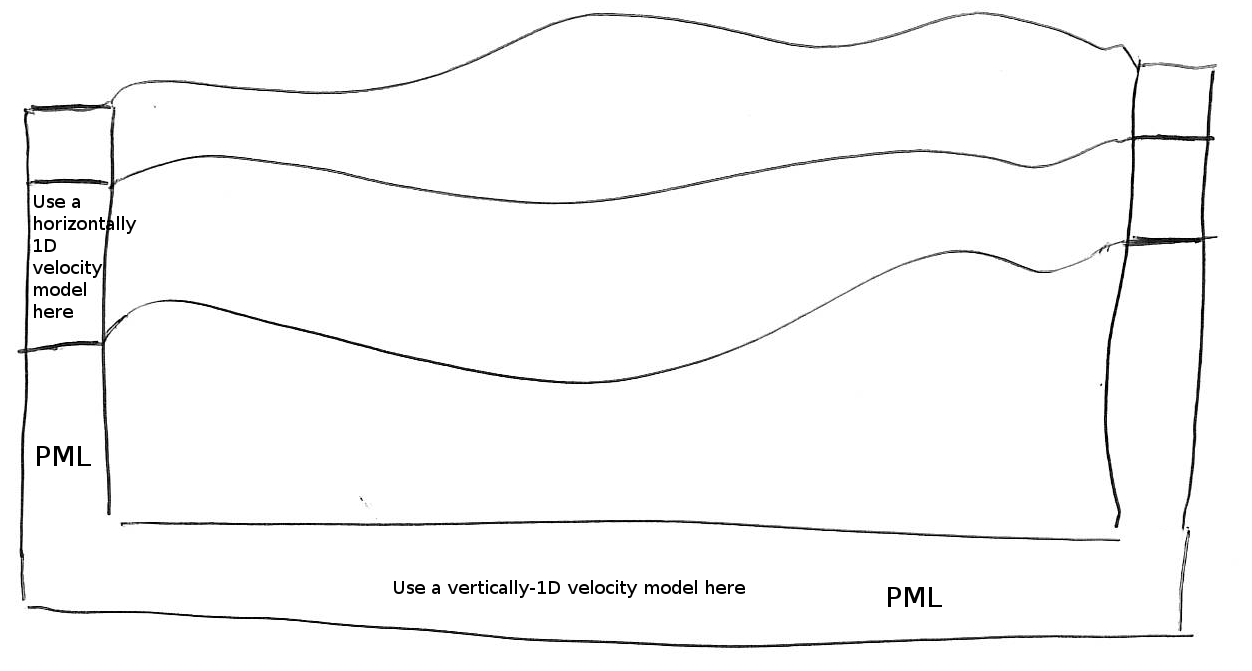
\includegraphics[width=3in]{figures/how_to_use_PML_when_a_tomographic_velocity_model_is_used}
\par\end{centering}

\caption{How to modify your external 3D velocity and density model in order
to use PML. Such a modification is not needed when using Stacey absorbing
boundary conditions (but such conditions are significantly less efficient).}


\label{fig:modify_external_velocity_model_to_use_PML}
\end{figure}


%%



\section{\label{sec:Choosing-the-Time-Step}Choosing the time step \texttt{DT}}

The parameter \texttt{DT} sets the length of each time step in seconds.
The value of this parameter is crucial for the stability of the spectral-element
simulation. Your time step \texttt{DT} will depend on the minimum
ratio between the distance $h$ of neighboring mesh points and the
wave speeds $v$ defined in your model. The condition for the time
step $\Delta t$ is:
\begin{lyxcode}
$\Delta t<C~\mathrm{min}_{\Omega}(~h/v~)$
\end{lyxcode}
where $C$ is the so-called Courant number and $\Omega$ denotes the
model volume. The distance $h$ depends on the mesh element size and
the number of GLL points \texttt{NGLL} specified in the main constants
file \texttt{constants.h} located in the \texttt{src/shared/} subdirectory.
The wave speed $v$ is determined based on your model's P- (or S-)
wave speed values.

The database generator \texttt{xgenerate\_databases}, as well as the
internal mesher \texttt{xmeshfem3D}, are trying to evaluate the value
of $\Delta t$ for empirically chosen Courant numbers $C\sim0.3$.
If you used the mesher \texttt{xmeshfem3D} to generate your mesh,
you should set the value suggested in \texttt{OUTPUT\_FILES/output\_mesher.txt}
file, which is created after the mesher completed. In case you used
CUBIT to create the mesh, you might use an arbitrary value when running
\texttt{xgenerate\_databases} and then use the value suggested in
the ~\\
 \texttt{OUTPUT\_FILES/output\_mesher.txt} file after the database
generation completed. Note that the implemented Newmark time scheme
uses this time step globally, thus your simulations become more expensive
for very small mesh elements in high wave-speed regions. Please be
aware of this restriction when constructing your mesh in Chapter~\ref{cha:Mesh-Generation}.


\chapter{\label{cha:Running-the-Solver}Running the Solver \texttt{xspecfem3D}}

Now that you have successfully generated the databases, you are ready
to compile the solver. In the main directory, type
\begin{lyxcode}
{\small make~xspecfem3D}{\small \par}
\end{lyxcode}
Please note that \texttt{xspecfem3D} must be called directly from
the \texttt{bin/} directory, as most of the binaries of the package.

The solver needs three input files in the \texttt{DATA} directory
to run:
\begin{description}
\item [{\texttt{Par\_file}}] the main parameter file which was discussed
in detail in the previous Chapter~\ref{cha:Creating-Distributed-Databases},
\item [{\texttt{CMTSOLUTION}} or {\texttt{FORCESOLUTION}}] the earthquake
source parameter file or the force source parameter file, and
\item [{\texttt{STATIONS}}] the stations file.
\end{description}
Most parameters in the \texttt{Par\_file} should be set prior to running
the databases generation. Only the following parameters may be changed
after running \texttt{xgenerate\_databases}:
\begin{itemize}
\item the simulation type control parameters: \texttt{SIMULATION\_TYPE}
and \texttt{SAVE\_FORWARD}
\item the time step parameters \texttt{NSTEP} and \texttt{DT}
\item the absorbing boundary control parameter \texttt{PML\_CONDITIONS}
on condition that the\\
 \texttt{PML\_INSTEAD\_OF\_FREE\_SURFACE} flag remains unmodified
after running the databases generation.
\item the movie control parameters \texttt{MOVIE\_SURFACE}, \texttt{MOVIE\_VOLUME},
and \texttt{NTSTEPS\_BETWEEN\_FRAMES}
\item the ShakeMap\textregistered{}option \texttt{CREATE\_SHAKEMAP}
\item the output information parameters \texttt{MOVIE\_TYPE}, \texttt{NTSTEP\_BETWEEN\_OUTPUT\_INFO}
and \texttt{NTSTEP\_BETWEEN\_OUTPUT\_}~\\
 \texttt{SEISMOS}
\item the \texttt{PRINT\_SOURCE\_TIME\_FUNCTION} flags
\end{itemize}
Any other change to the \texttt{Par\_file} implies rerunning both
the database generator \texttt{xgenerate\_databases} and the solver
\texttt{xspecfem3D}.

For any particular earthquake, the \texttt{CMTSOLUTION} file that
represents the point source may be obtained directly from the Harvard
Centroid-Moment Tensor (CMT) web page \urlwithparentheses{www.seismology.harvard.edu}.
It looks like this:
\begin{lyxcode}
\begin{figure}[H]
\noindent \begin{centering}
{\small 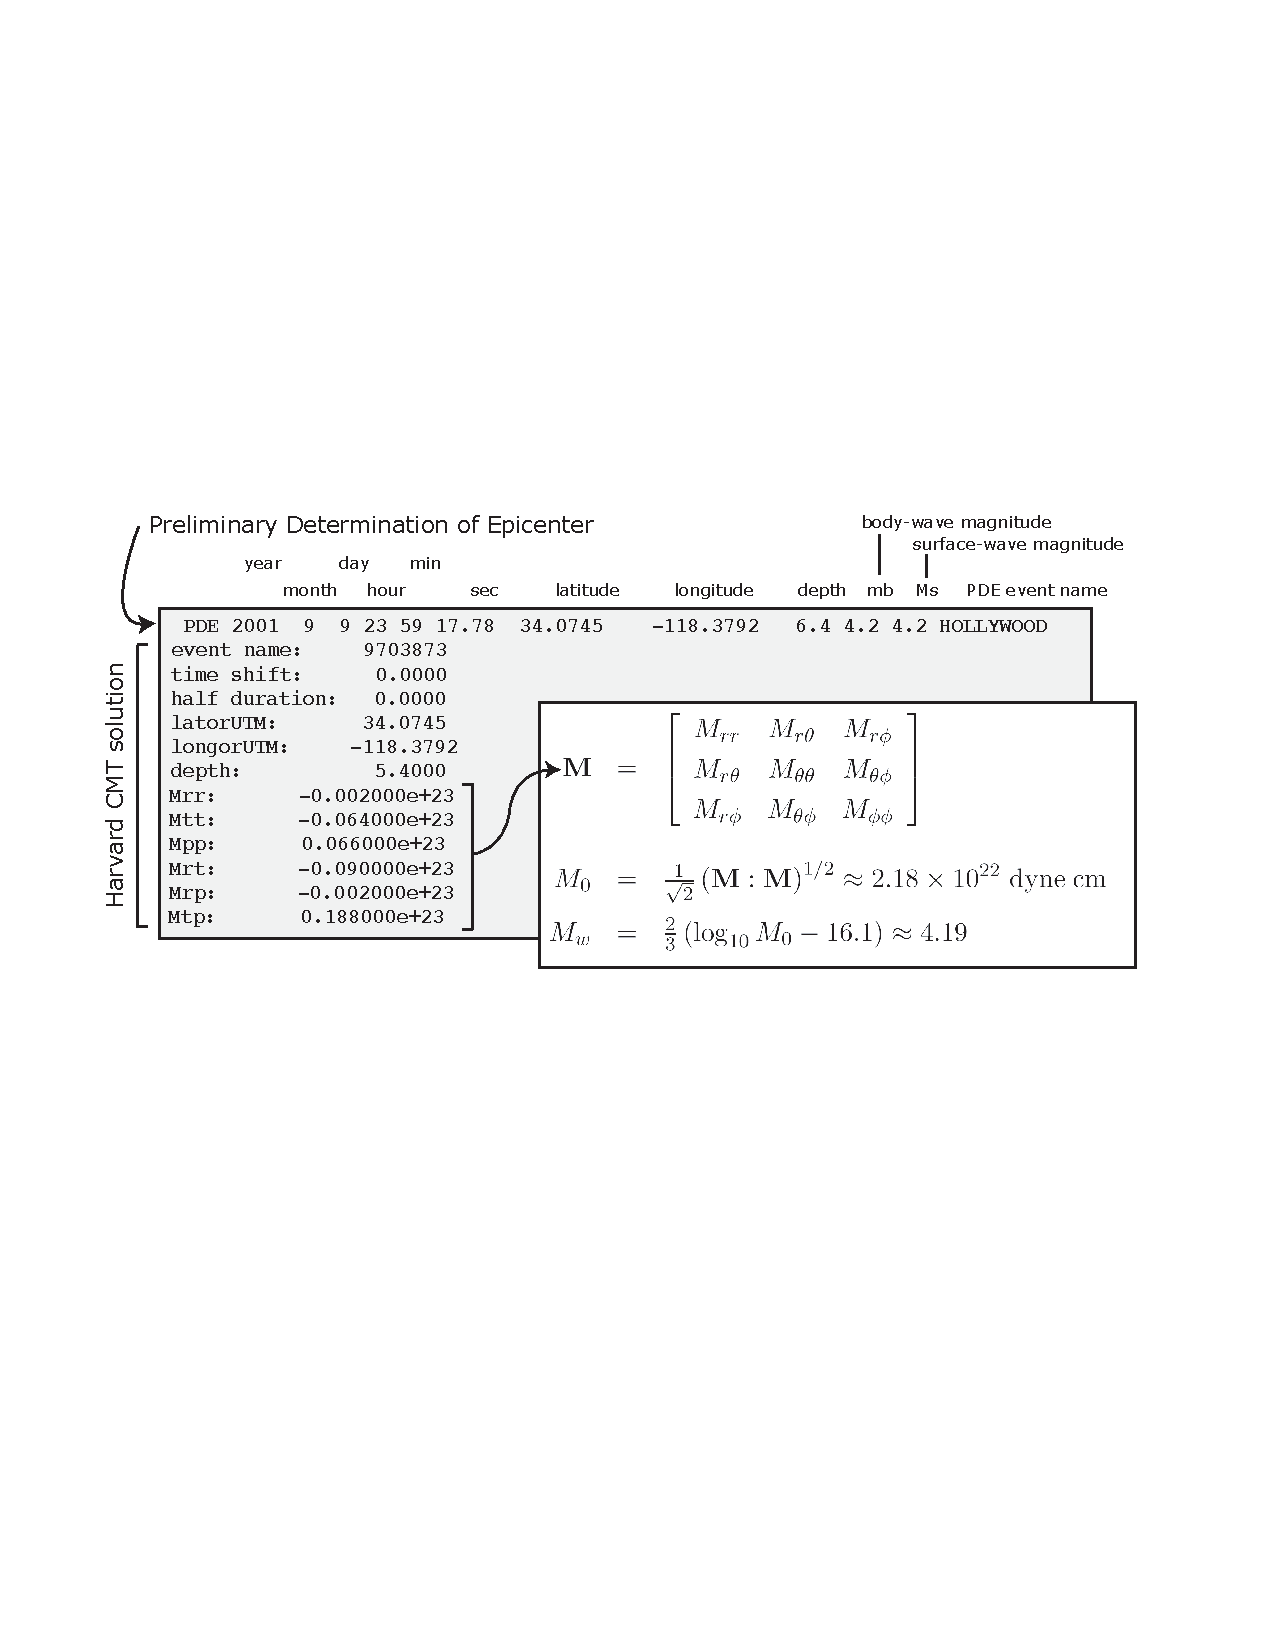
\includegraphics[width=1\textwidth]{figures/Hollywood_CMT}
}
\par\end{centering}



\caption{\label{fig:CMTSOLUTION-file}\texttt{CMTSOLUTION} file based on the
format from the Harvard CMT catalog. \textbf{M} is the moment tensor,
$M_{0}${\small {} }is the seismic moment, and $M_{w}$ is the moment
magnitude.}
\end{figure}



\end{lyxcode}
The \texttt{CMTSOLUTION} file should be edited in the following way:
\begin{itemize}
\item Set the \texttt{time shift} parameter equal to $0.0$ (the solver
will not run otherwise.) The time shift parameter would simply apply
an overall time shift to the synthetics, something that can be done
in the post-processing (see Section \ref{sec:Process-data-and-syn}).
\item For point-source simulations (see finite sources, page \pageref{To-simulate-a})
we recommend setting the source half-duration parameter \texttt{half
duration} equal to zero, which corresponds to simulating a step source-time
function, i.e., a moment-rate function that is a delta function. If
\texttt{half duration} is not set to zero, the code will use a Gaussian
(i.e., a signal with a shape similar to a `smoothed triangle', as
explained in \citet{KoTr02a} and shown in Fig~\ref{fig:gauss.vs.triangle})
source-time function with half-width \texttt{half duration}. We prefer
to run the solver with \texttt{half duration} set to zero and convolve
the resulting synthetic seismograms in post-processing after the run,
because this way it is easy to use a variety of source-time functions
(see Section \ref{sec:Process-data-and-syn}). \citet{KoTr02a} determined
that the noise generated in the simulation by using a step source
time function may be safely filtered out afterward based upon a convolution
with the desired source time function and/or low-pass filtering. Use
the serial code \texttt{convolve\_source\_timefunction.f90} and the
script \texttt{convolve\_source\_timefunction.csh} for this purpose,
or alternatively use signal-processing software packages such as SAC
\urlwithparentheses{www.llnl.gov/sac}. Type

\begin{lyxcode}
{\small make~xconvolve\_source\_timefunction}{\small \par}
\end{lyxcode}

to compile the code and then set the parameter \texttt{hdur} in \texttt{convolve\_source\_timefunction.csh}
to the desired half-duration.

\item The zero time of the simulation corresponds to the center of the triangle/Gaussian,
or the centroid time of the earthquake. The start time of the simulation
is $t=-1.5*\texttt{half duration}$ (the 1.5 is to make sure the moment
rate function is very close to zero when starting the simulation).
To convert to absolute time $t_{\mathrm{abs}}$, set

\begin{lyxcode}
$t_{\mathrm{abs}}=t_{\mathrm{pde}}+\texttt{time shift}+t_{\mathrm{synthetic}}$
\end{lyxcode}

where $t_{\mathrm{pde}}$ is the time given in the first line of the
\texttt{CMTSOLUTION}, \texttt{time shift} is the corresponding value
from the original \texttt{CMTSOLUTION} file and $t_{\mathrm{synthetic}}$
is the time in the first column of the output seismogram.

\end{itemize}
\begin{figure}
\noindent \begin{centering}
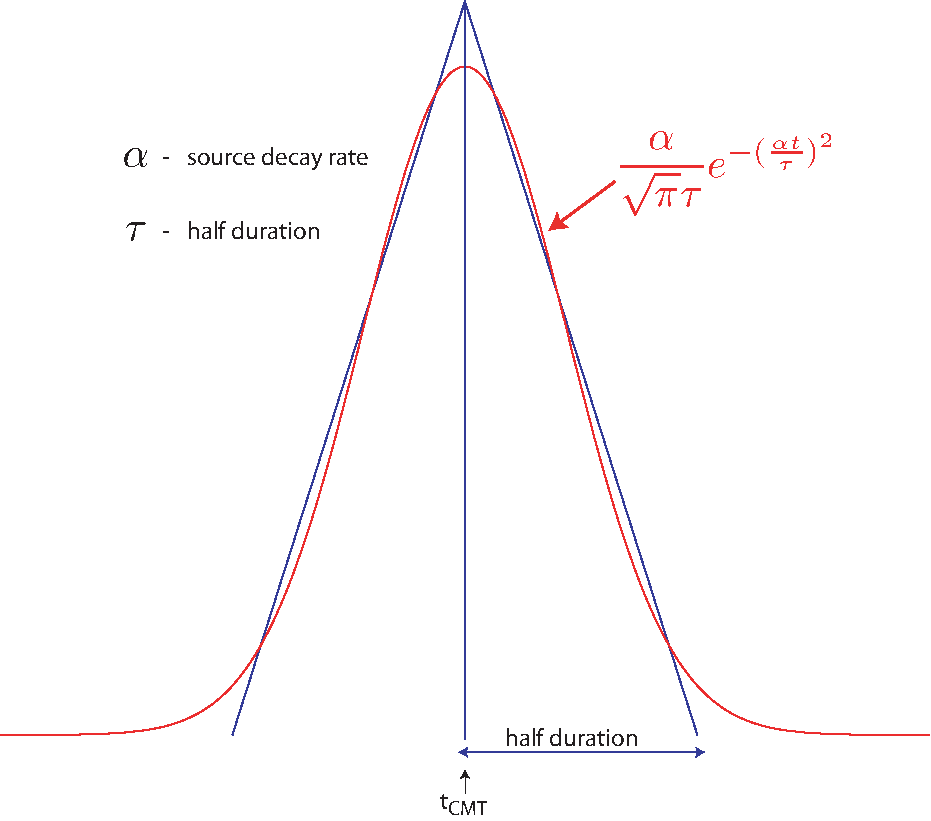
\includegraphics[width=2.5in]{figures/gauss_vs_triangle_mod}
\par\end{centering}

\caption{Comparison of the shape of a triangle and the Gaussian function actually
used.}


\label{fig:gauss.vs.triangle}
\end{figure}


If you know the earthquake source in strike/dip/rake format rather
than in \texttt{CMTSOLUTION} format, use the C code \texttt{SPECFEM3D\_GLOBE/utils/strike\_dip\_rake\_to\_CMTSOLUTION.c}
to convert it. The conversion formulas are given for instance in \citet{AkRi80}.
Note that the \citet{AkRi80} convention is slightly different from
the Harvard \texttt{CMTSOLUTION} convention (the sign of some components
is different). The C code outputs both.

Centroid latitude and longitude should be provided in geographical
coordinates. The code converts these coordinates to geocentric coordinates~\citep{DaTr98}.
Of course you may provide your own source representations by designing
your own \texttt{CMTSOLUTION} file. Just make sure that the resulting
file adheres to the Harvard CMT conventions (see Appendix~\ref{cha:Coordinates}).
Note that the first line in the \texttt{CMTSOLUTION} file is the Preliminary
Determination of Earthquakes (PDE) solution performed by the USGS
NEIC, which is used as a seed for the Harvard CMT inversion. The PDE
solution is based upon P waves and often gives the hypocenter of the
earthquake, i.e., the rupture initiation point, whereas the CMT solution
gives the `centroid location', which is the location with dominant
moment release. The PDE solution is not used by our software package
but must be present anyway in the first line of the file.

\label{To-simulate-a}To simulate a kinematic rupture, i.e., a finite-source
event, represented in terms of $N_{\mathrm{sources}}$ point sources,
provide a \texttt{CMTSOLUTION} file that has $N_{\mathrm{sources}}$
entries, one for each subevent (i.e., concatenate $N_{\mathrm{sources}}$
\texttt{CMTSOLUTION} files to a single \texttt{CMTSOLUTION} file).
At least one entry (not necessarily the first) must have a zero \texttt{time
shift}, and all the other entries must have non-negative \texttt{time
shift}. Each subevent can have its own half duration, latitude, longitude,
depth, and moment tensor (effectively, the local moment-density tensor).

Note that the zero in the synthetics does NOT represent the hypocentral
time or centroid time in general, but the timing of the \textit{center}
of the source triangle with zero \texttt{time shift} (Fig~\ref{fig:source_timing}).

Although it is convenient to think of each source as a triangle, in
the simulation they are actually Gaussians (as they have better frequency
characteristics). The relationship between the triangle and the gaussian
used is shown in Fig~\ref{fig:gauss.vs.triangle}. For finite fault
simulations it is usually not advisable to use a zero half duration
and convolve afterwards, since the half duration is generally fixed
by the finite fault model.

\vspace{1cm}


\noindent The \texttt{FORCESOLUTION} file should be edited in the
following way:
\begin{itemize}
\item Set the \texttt{time shift} parameter equal to $0.0$ (the solver
will not run otherwise.) The time shift parameter would simply apply
an overall time shift to the synthetics, something that can be done
in the post-processing (see Section \ref{sec:Process-data-and-syn}).
\item Set the \texttt{half duration} parameter of the Ricker source time
function when {\texttt{USE\_RICKER\_TIME\_FUNCTION}} is turned on
in the main parameter file {\texttt{Par\_file}}. In case that the
solver uses a (pseudo) Dirac delta source time function to represent
a force point source, a very short \texttt{half duration} parameter
(hdur = 5 {*} DT) is automatically set by default.
\item Set the latitude, longitude, depth of the source in geographical coordinates.
\item Set the magnitude of the force source.
\item Set the components of a (non-unitary) direction vector for the force
source in the East/North/Vertical basis (see Appendix A for the orientation
of the reference frame).
\end{itemize}
\noindent Where necessary, set a \texttt{FORCESOLUTION} file in the
same way you configure a \texttt{CMTSOLUTION} file with $N_{\mathrm{sources}}$
entries, one for each subevent (i.e., concatenate $N_{\mathrm{sources}}$
\texttt{FORCESOLUTION} files to a single \texttt{FORCESOLUTION} file).
At least one entry (not necessarily the first) must have a zero \texttt{time
shift}, and all the other entries must have non-negative \texttt{time
shift}. Each subevent can have its own half latitude, longitude, depth,
\texttt{half duration} and force parameters.

\begin{figure}[H]
\noindent \begin{centering}
{\small 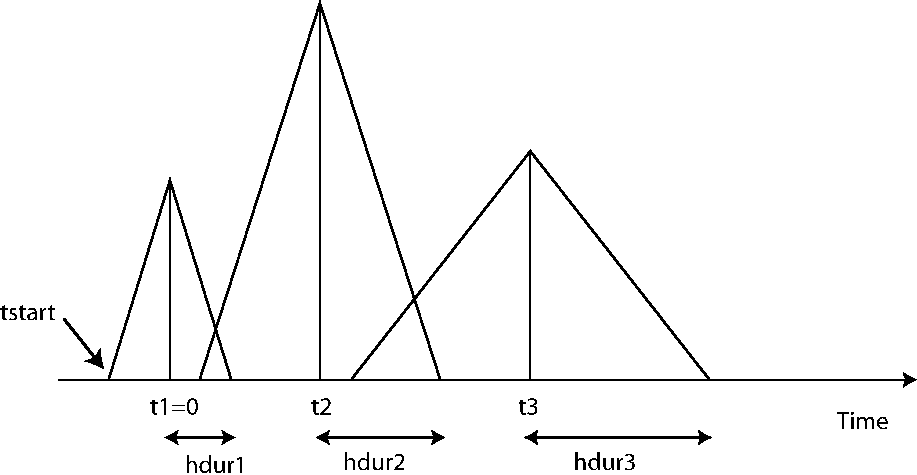
\includegraphics[width=5in]{figures/source_timing} }
\par\end{centering}



\caption{Example of timing for three sources. The center of the first source
triangle is defined to be time zero. Note that this is NOT in general
the hypocentral time, or the start time of the source (marked as tstart).
The parameter \texttt{time shift} in the \texttt{CMTSOLUTION} file
would be t1(=0), t2, t3 in this case, and the parameter \texttt{half
duration} would be hdur1, hdur2, hdur3 for the sources 1, 2, 3 respectively.}


{\small \label{fig:source_timing} }
\end{figure}




The solver can calculate seismograms at any number of stations for
basically the same numerical cost, so the user is encouraged to include
as many stations as conceivably useful in the \texttt{STATIONS} file,
which looks like this:

\begin{figure}[H]
\noindent \begin{centering}
{\small 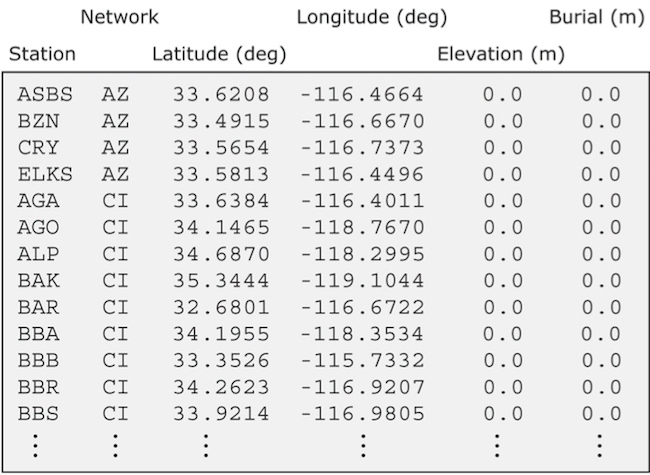
\includegraphics{figures/STATIONS_basin_explained} }
\par\end{centering}



\label{fig:Sample-STATIONS-file.}\caption{Sample \texttt{STATIONS} file. Station latitude and longitude should
be provided in geographical coordinates. The width of the station
label should be no more than 32 characters (see \texttt{MAX\_LENGTH\_STATION\_NAME}
in the \texttt{constants.h} file), and the network label should be
no more than 8 characters (see \texttt{MAX\_LENGTH\_NETWORK\_NAME}
in the \texttt{constants.h} file).}
\end{figure}




Each line represents one station in the following format:
\begin{lyxcode}
{\small Station~Network~Latitude~(degrees)~Longitude~(degrees)~Elevation~(m)~burial~(m)~}{\small \par}
\end{lyxcode}
The solver \texttt{xspecfem3D} filters the list of stations in file
\texttt{DATA/STATIONS} to exclude stations that are not located within
the region given in the \texttt{Par\_file} (between \texttt{LATITUDE\_MIN}
and \texttt{LATITUDE\_MAX} and between \texttt{LONGITUDE\_MIN} and
\texttt{LONGITUDE\_MAX}). The filtered file is called \texttt{DATA/STATIONS\_FILTERED}.

Solver output is provided in the \texttt{OUTPUT\_FILES} directory
in the \texttt{output\_solver.txt} file. Output can be directed to
the screen instead by uncommenting a line in \texttt{constants.h}:
\begin{lyxcode}
!~uncomment~this~to~write~messages~to~the~screen~

!~integer,~parameter~::~IMAIN~=~ISTANDARD\_OUTPUT~
\end{lyxcode}
On PC clusters the seismogram files are generally written to the local
disks (the path \texttt{LOCAL\_PATH} in the \texttt{Par\_file}) and
need to be gathered at the end of the simulation.

While the solver is running, its progress may be tracked by monitoring
the `\texttt{\small timestamp{*}}{\small ' files in the ~}\\
{\small{} }\texttt{\small OUTPUT\_FILES}{\small{} directory. These tiny
files look something like this:}{\small \par}
\begin{lyxcode}
Time~step~\#~~~~~~~~~~10000~

Time:~~~~~108.4890~~~~~~seconds~

Elapsed~time~in~seconds~=~~~~1153.28696703911~

Elapsed~time~in~hh:mm:ss~=~~~~~0~h~19~m~13~s~

Mean~elapsed~time~per~time~step~in~seconds~=~~~~~0.115328696703911~

Max~norm~displacement~vector~U~in~all~slices~(m)~=~~~~1.0789589E-02~
\end{lyxcode}
The \texttt{\small timestamp{*}}{\small{} files provide the }\texttt{\small Mean
elapsed time per time step in seconds}{\small , which may be used
to assess performance on various machines (assuming you are the only
user on a node), as well as the }\texttt{\small Max norm displacement
vector U in all slices~(m)}{\small . If something is wrong with the
model, the mesh, or the source, you will see the code become unstable
through exponentially growing values of the displacement and fluid
potential with time, and ultimately the run will be terminated by
the program. You can control the rate at which the timestamp files
are written based upon the parameter }\texttt{\small NTSTEP\_BETWEEN\_OUTPUT\_INFO}{\small{}
in the }\texttt{\small Par\_file}{\small .}{\small \par}

Having set the \texttt{Par\_file} parameters, and having provided
the \texttt{CMTSOLUTION} (or the \texttt{FORCESOLUTION}) and \texttt{STATIONS}
files, you are now ready to launch the solver! This is most easily
accomplished based upon the \texttt{go\_solver} script (See Chapter
\ref{cha:Scheduler} for information about running through a scheduler,
e.g., LSF). You may need to edit the last command at the end of the
script that invokes the \texttt{mpirun} command. The \texttt{runall}
script compiles and runs both \texttt{xgenerate\_databases} and \texttt{xspecfem3D}
in sequence. This is a safe approach that ensures using the correct
combination of distributed database output and solver input.

It is important to realize that the CPU and memory requirements of
the solver are closely tied to choices about attenuation (\texttt{ATTENUATION})
and the nature of the model (i.e., isotropic models are cheaper than
anisotropic models). We encourage you to run a variety of simulations
with various flags turned on or off to develop a sense for what is
involved.

For the same model, one can rerun the solver for different events
by simply changing the \texttt{CMTSOLUTION} or \texttt{FORCESOLUTION}
file, or for different stations by changing the \texttt{STATIONS}
file. There is no need to rerun the \texttt{xgenerate\_databases}
executable. Of course it is best to include as many stations as possible,
since this does not add to the cost of the simulation.


\chapter{\label{cha:Fault-Kinematics-Dynamics}Kinematic and dynamic fault
sources}

SPECFEM3D can handle finite fault sources of two kinds:
\begin{enumerate}
\item \emph{Kinematic}: the spatio-temporal distribution of slip rate is
prescribed along the fault surface
\item \emph{Dynamic}: a friction law and initial stresses are prescribed
on the fault, a spontaneous rupture process is computed.
\end{enumerate}

\section{\label{sec:Mesh-Generation-with}Mesh Generation with Split Nodes}

Faults need to be handled in a special way during mesh generation.
A fault surface must lie at the interface between elements (the mesh
must honor the fault surfaces). Moreover, a fault is made of two surfaces
in contact. Each of these two surfaces needs a separate set of nodes.
This approach is known as \textquotedbl{}split nodes\textquotedbl{}.
Currently faults can only be run with \texttt{xdecompose\_mesh }and\texttt{
CUBIT. xmeshfem3D }is not yet ready to handle faults.\\
To facilitate the mesh generation with split nodes in CUBIT, we need
to separate the two fault surfaces by a small distance, effectively
creating a tiny opening of the fault (Figure \ref{fig:examples.splitnodes},
\ref{fig:examples.splitnodes-surfacetrace}). Note that only the interior
of the fault must be opened, its edges must remain closed (except
the edge on the free surface). The fault is automatically closed later
by SPECFEM3D.\\


Here is an example CUBIT script to generate a mesh with split nodes
for a buried vertical strike-slip fault:
\begin{lyxcode}
~reset~~\\
~brick~x~10~y~10~z~10~~\\
~webcut~volume~all~with~plane~xplane~~\\
~webcut~volume~all~with~plane~yplane~~\\
~webcut~volume~all~with~plane~xplane~offset~3~~\\
~webcut~volume~all~with~plane~zplane~offset~3~~\\
~webcut~volume~all~with~plane~zplane~offset~-3~~\\
~imprint~all~~\\
~merge~all~~\\
~unmerge~surf~160~~\\
~mesh~vol~all~~\\
~set~node~constraint~off~~\\
~node~in~surf~168~move~X~0~Y~0.01~Z~0~~\\
~node~in~surf~160~move~X~0~Y~-0.01~Z~0~\\

\end{lyxcode}
\begin{figure}[htbp]
\noindent \begin{centering}
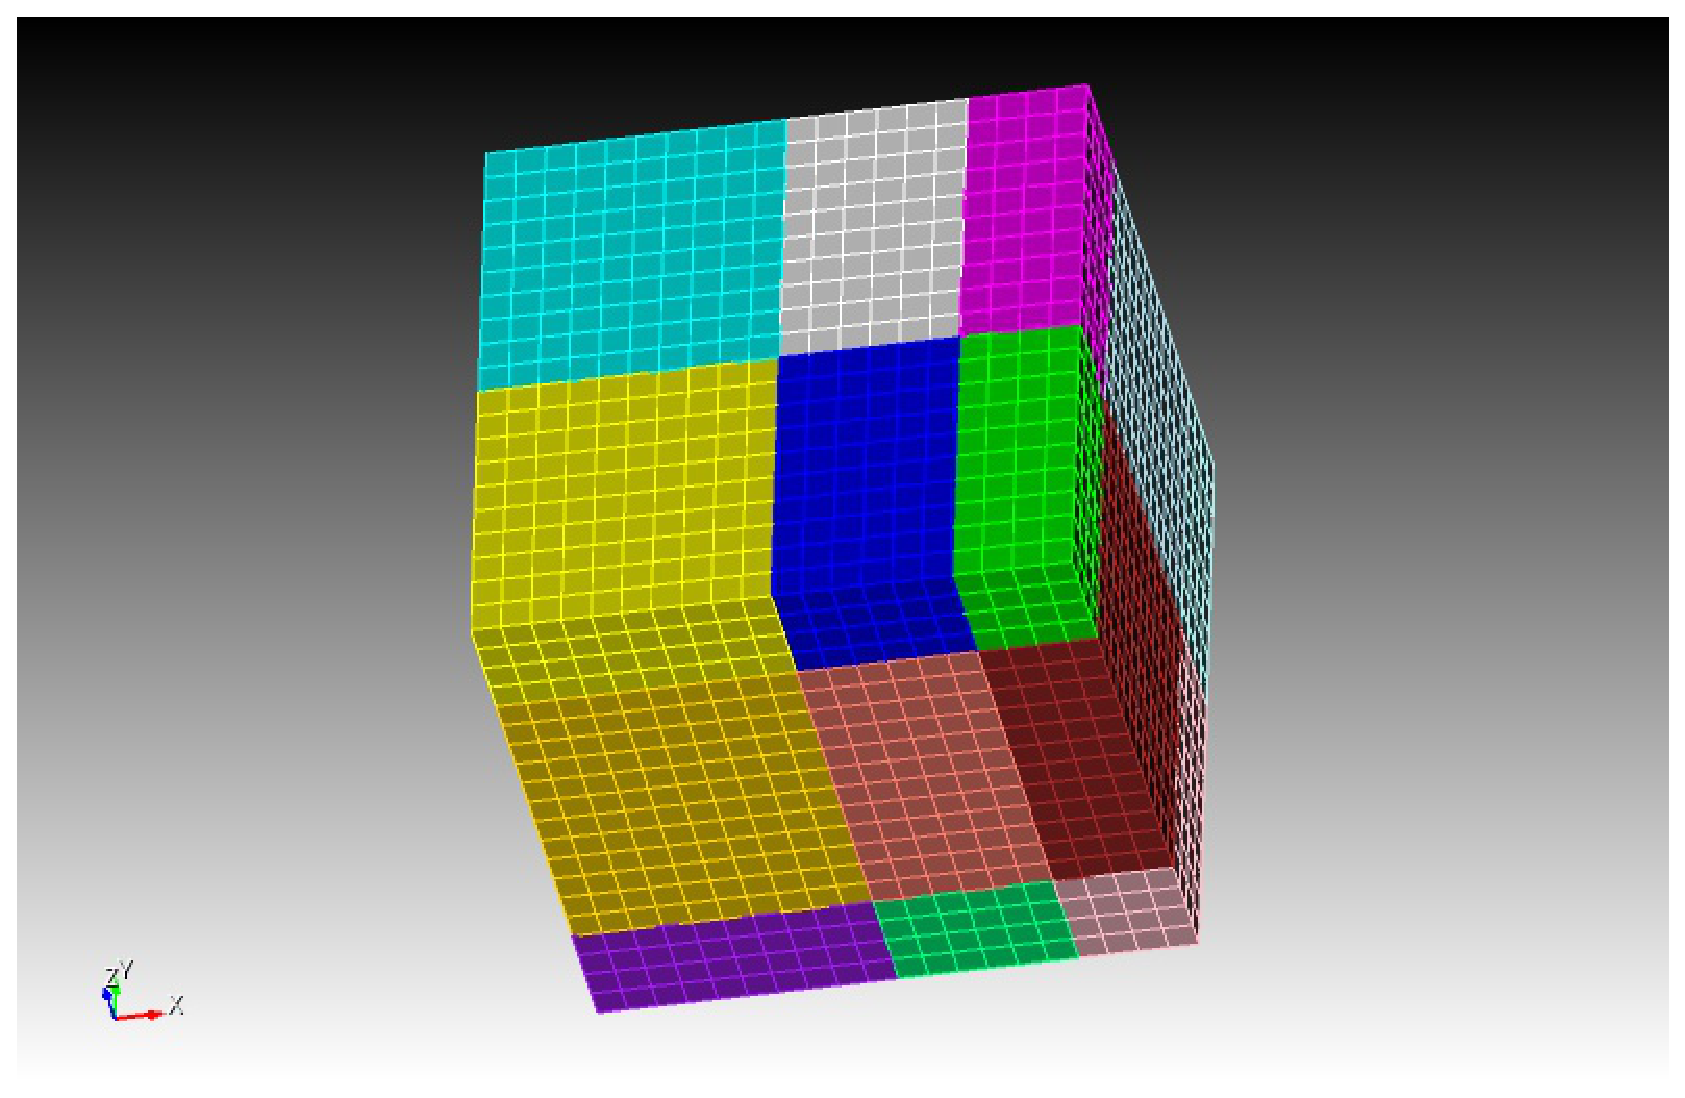
\includegraphics[scale=0.3]{figures/faultmesh} \\
 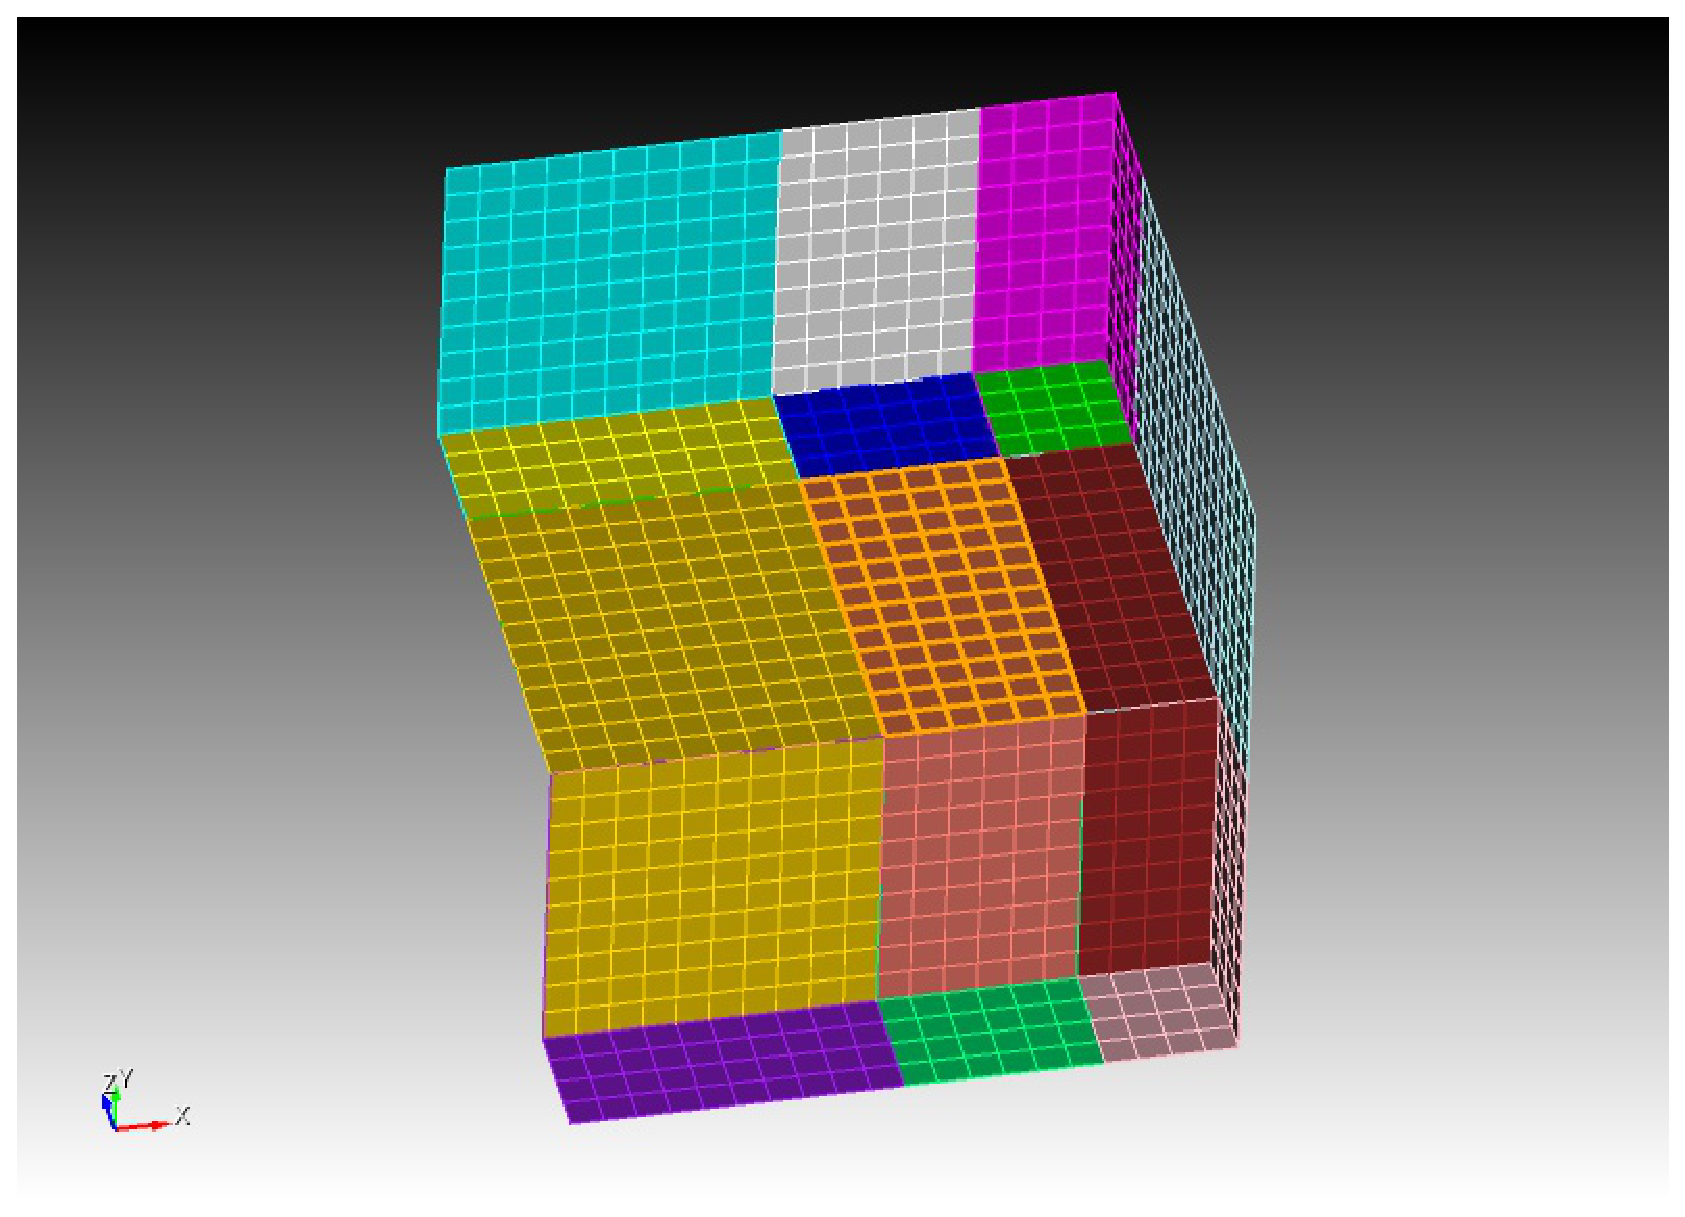
\includegraphics[scale=0.3]{figures/surf168} 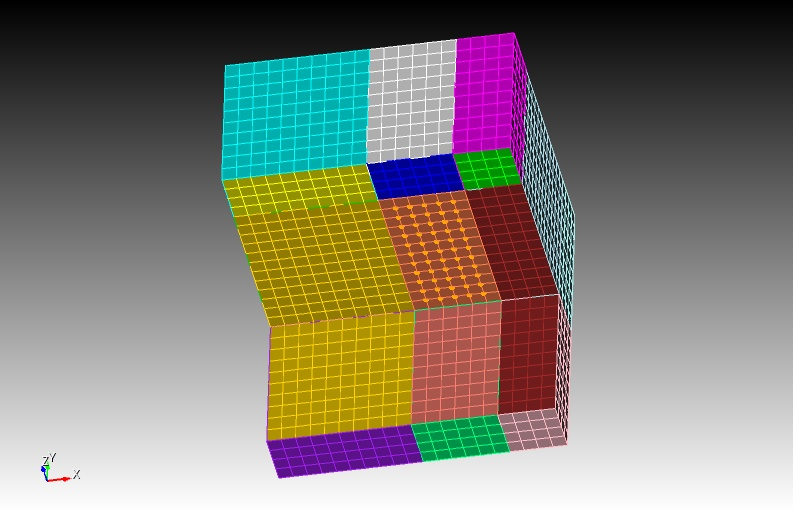
\includegraphics[scale=0.3]{figures/splitnodes}
\par\end{centering}

\caption{Screenshots of the CUBIT example for the embedded fault with split
nodes: The entire mesh is decomposed into several volumes bounding
the fault (top), the fault surface 168 is shown as orange squares
(middle) and split nodes of the fault shown as orange dots(bottom).
Note that only interior nodes of the fault are split while those on
the edges of the fault surface are touching each other.}


\label{fig:examples.splitnodes}
\end{figure}

\begin{lyxcode}

\end{lyxcode}
\begin{figure}[htbp]
\noindent \begin{centering}
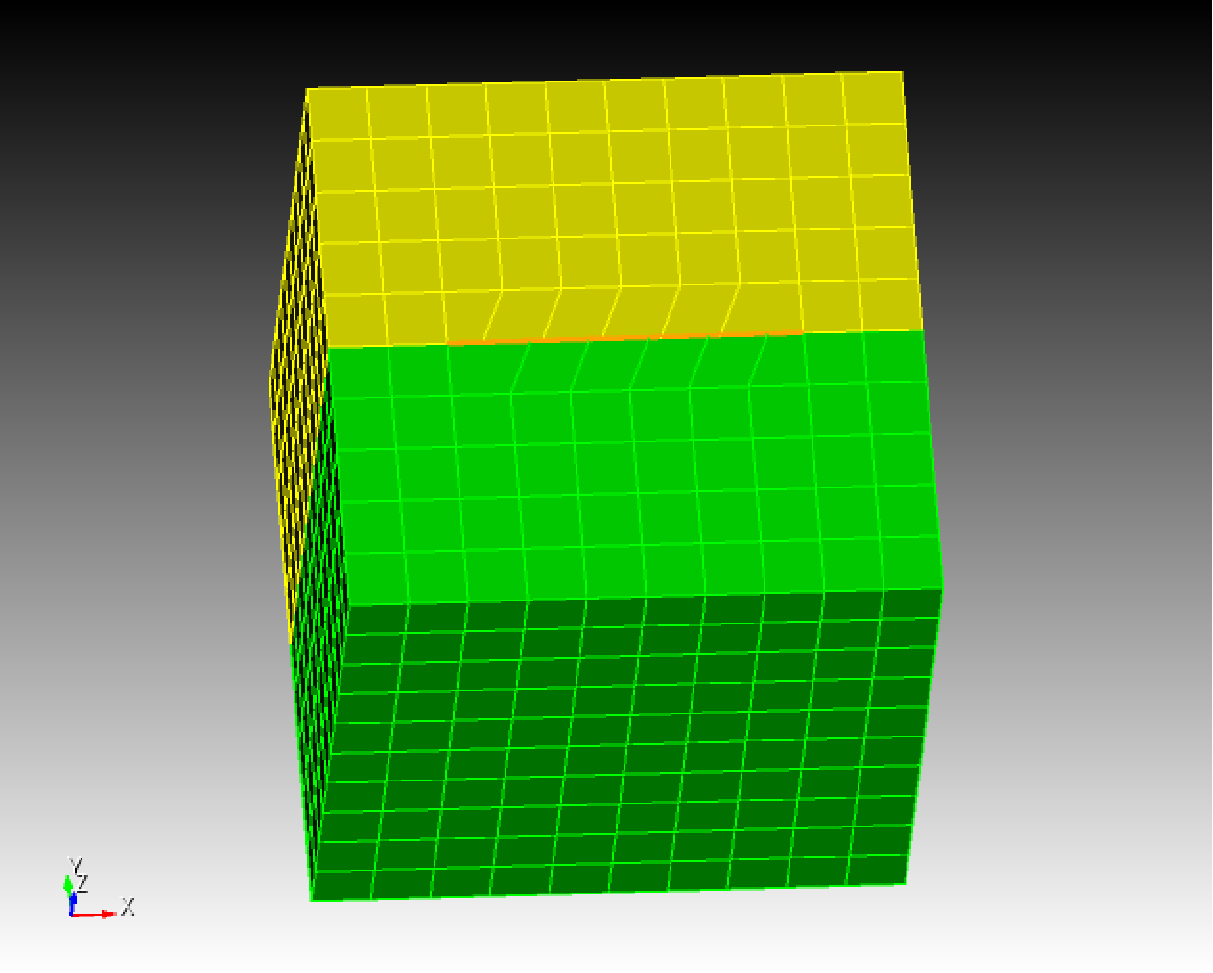
\includegraphics[scale=0.55]{figures/splitnodes_surfacetrace} \\

\par\end{centering}

\caption{Screenshots of a CUBIT example showing split nodes for a fault reaching
the surface. Surface trace of the fault is shown in orange. Note that
the edges of the fault are not split while the interior nodes are
offset by a small distance on either side of the fault}


\label{fig:examples.splitnodes-surfacetrace}
\end{figure}


The CUBIT scripts ({*}.jou and {*}.py) in the directory $\mathtt{examples}$
generate more complicated meshes. The {*}.py files are Python scripts
that execute CUBIT commands and use the CUBIT-python interface for
SPECFEM3D (see next section). The Python language allows to define
and manipulate variables to parameterize the mesh. Alternatively,
the Python script can call a CUBIT journal file ({*}.jou), which looks
like the example above. Variables can be defined and manipulated there
using the $\mathtt{APREPRO}$ language built in CUBIT.\\


Note that you should avoid gaps in the list of indices of mesh objects
with the following CUBIT command:
\begin{lyxcode}
$\mathtt{compress\: ids\: hex\: face\: edge\: node}$
\end{lyxcode}
(otherwise you will get a segmentation fault during domain decomposition)


\section{CUBIT-Python Scripts for Faults}

The mesh generated in CUBIT needs to be processed and exported in
a format compatible with SPECFEM3D. This is achieved in the Python
scripts by calling the Python-CUBIT interface functions defined in
the CUBIT directory:
\begin{enumerate}
\item Function $\mathtt{define\_bc}$ (or $\mathtt{boundary\_definition.py}$)
must be called to set up the absorbing boundaries database
\item Function $\mathtt{fault\_input}$ must be called once for each fault
to set up the fault database
\item Function $\mathtt{cubit2specfem3d.export2SPECFEM3D}$ must be called
at the very end of the script to export the mesh in a SPECFEM3D format.
\end{enumerate}
The functions in \#1 and \#3 are for the bulk and are documented in
Section \ref{subsec:Exporting-the-Mesh}. We focus here on \#2:
\begin{description}
\item [{Function:}] $\mathtt{fault\_input}$
\item [{Purpose:}] export a fault mesh database from CUBIT to a SPECFEM3D-compliant
file
\item [{Syntax:}] fault\_input(id\_fault, ids\_surf\_1, ids\_surf\_2)
\item [{Inputs:}]~\end{description}
\begin{itemize}
\item id\_fault integer index assigned to the fault. (The user must number
all the faults, starting at 1, with unit increments)
\item ids\_surf\_1 list of CUBIT ids of all surfaces that form side 1 of
the fault.
\item ids\_surf\_2 list of CUBIT ids of all surfaces that form side 2 of
the fault. (The user must decide which side of the fault is side 1.
This choice affects the sign conventions of fault quantities as explained
in Section \ref{sec:Sign-Convention-for}).\end{itemize}
\begin{description}
\item [{Outputs:}] file $\mathtt{fault\_file\_X.dat}$, where X is the
fault id (id\_fault).
\item [{Example:}] For the example in Section \ref{sec:Mesh-Generation-with}:\end{description}
\begin{lyxcode}
$\hphantom{}$A1~=~{[}168{]}

$\hphantom{}$A2~=~{[}160{]}

$\hphantom{}$fault\_input(1,A1,A2)
\end{lyxcode}

\section{Examples}

The package includes examples, the SCEC benchmark problems:
\begin{itemize}
\item TPV5, a planar vertical strike-slip fault
\item TPV14 and TPV15, vertical strike-slip fault system with a fault branch
\item TPV102 and TPV103, rate-and-state benchmarks
\item TPV22 and TPV23, step-over benchmarks
\item TPV16, heterogenous initial stress
\end{itemize}
and
\begin{itemize}
\item Splay fault models from Wendt et al. (2009)\\

\end{itemize}
Read the documents in the directory $\mathtt{examples/*/description}$.
They contain a description of the example and additional instructions
to run it. Visualize the results with the Matlab scripts in the directory
$\mathtt{examples/*/post}$


\section{\label{sec:Sign-Convention-for}Sign Convention for Fault Quantities}

During mesh generation, the fault is defined by two surfaces in contact.
Let's denote as \textquotedbl{}\emph{side 1}\textquotedbl{} the SECOND
surface declared by the user in the call to the python function \textquotedbl{}\emph{fault\_input}\textquotedbl{},
and the FIRST surface as \textquotedbl{}\emph{side 2}\textquotedbl{}.
The local coordinate system on the fault is defined as the right-handed
coordinate system defined by (strike, dip, normal), where \textquotedbl{}\emph{normal}\textquotedbl{}
is the normal vector outgoing from side 1, \textquotedbl{}\emph{dip}\textquotedbl{}
is parallel to the along-dip direction pointing downwards, and \textquotedbl{}\emph{strike}\textquotedbl{}
is the horizontal along-strike vector such that the system is right-handed.\\


Slip is defined as displacement on side 2 minus displacement on side
1. In the local coordinate system on the fault, positive along-strike
slip is right-lateral and positive along-dip slip is thrust if side
1 is on the hanging wall (normal faulting if side 1 is on the foot
wall).\\


Traction is defined as the stress induced on side 1 by side 2, which
is the stress tensor times the normal vector outgoing from side 1.
In the local coordinate system on the fault, the normal traction is
negative in compression, positive along-strike traction generates
right-lateral slip and positive along-dip traction generates thrust
slip if side 1 is on the hanging wall (normal faulting if side 1 is
on the foot wall).


\section{Input Files}

Three additional input files are required in the \texttt{DATA} directory
for dynamic and kinematic faults. They are $\mathtt{Par\_file\_faults}$,
$\mathtt{FAULT\_STATIONS}$ and $\mathtt{input\_file.txt}$ (optional).
If the former does not exist, the code assumes that there are no faults.\\

\begin{lyxlist}{00.00.0000}
\item [{\textbf{DATA/Par\_file\_faults}}] contains parameters of the fault.
The first part of this file has a strict format:

\begin{description}
\item [{Line}] 1: Number of faults (NF)
\item [{Lines}] 2 to NF+1: Kelvin Voigt damping (in seconds) for each fault.
(See below how to set this parameter)
\item [{Line}] NF+2: Type of simulation (1=dynamic , 2 = kinematic)
\item [{Line}] NF+3: Number of time steps between updates of the time series
outputs at selected fault points (see DATA/FAULT\_STATIONS), usually
a large number (100s or 1000s). Note that the sampling rate of the
time series is usually much higher.
\item [{Line}] NF+4: Number of time steps between fault snapshot outputs
(quantities at every fault point exported at regular times), usually
a large number (100s or 1000s).
\item [{Line}] NF+5: Slip velocity threshold below which frictional healing
is set (friction coefficient is reset to its static value). If this
value is negative healing is disabled.
\item [{Line}] NF+6: Slip velocity threshold to define the rupture front.
Only used for outputs.
\end{description}

The rest of this file is made of namelist input blocks (see \textquotedbl{}namelist\textquotedbl{}
in a Fortran 9x manual). The input for each fault has the following
sequence (arguments in {[}brackets{]} are optional):


\&\textbf{BEGIN\_FAULT} /


\&\textbf{INIT\_STRESS} S1, S2, S3 {[},n1, n2, n3{]} /


followed by (n1+n2+n3) \&\textbf{DIST2D} blocks


\&\textbf{SWF} mus, mud, dc {[}, nmus, nmud, ndc{]} /


followed by (nmus+nmud+ndc) \&\textbf{DIST2D} blocks\\

\begin{lyxlist}{00.00.0000}
\item [{\&\textbf{INIT\_STRESS}}] input block sets the initial fault stresses
relative to the foot-wall side of the fault. Initial stresses are
composed of a constant background value possibly overwritten in prescribed
regions by heterogeneous distributions (see \&\textbf{DIST2D} blocks
below):

\begin{description}
\item [{S1}] = constant background value of along-strike shear stress (positive
in the usual strike direction)
\item [{S2}] = constant background value of along-dip shear (positive is
down-dip, normal faulting)
\item [{S3}] = constant background value of normal stress (negative in
compression)
\item [{n1}] = number of heterogeneous items for along-strike shear stress
{[}default is 0{]}
\item [{n2}] = number of heterogeneous items for along-dip shear stress
{[}default is 0{]}
\item [{n3}] = number of heterogeneous items for normal stress {[}default
is 0{]}
\end{description}
\item [{\&\textbf{SWF}}] input block sets the slip-weakening friction parameters
of the fault:

\begin{description}
\item [{mus}] = constant background value of static friction coefficient
\item [{mud}] = constant background value of dynamic friction coefficient
\item [{dc}] = constant background value of critical slip-weakening distance
\item [{nmus}] = number of heterogeneous items for static friction coefficient
{[}default is 0{]}
\item [{nmud}] = number of heterogeneous items for dynamic friction coefficient
{[}default is 0{]}
\item [{ndc}] = number of heterogeneous items for critical slip-weakening
distance {[}default is 0{]}\\

\end{description}
\item [{\&\textbf{DIST2D}}] input blocks modify (overwrite) the value of
a fault parameter by a heterogeneous spatial distribution:


\&\textbf{DIST2D} shape='$\mathtt{square}$', val, xc, yc, zc, l /


$\;$sets a constant value (val) within a cube with center (xc,yc,zc)
and edge size l.


\&\textbf{DIST2D} shape='$\mathtt{rectangle}$', val, xc, yc, zc,
lx, ly, lz /


$\;$sets a constant value (val) within a rectangular prism with center
(xc,yc,zc) and edge sizes (lx,ly,lz).


\&\textbf{DIST2D} shape='$\mathtt{rectangle-taper}$', val, valh,
xc, yc, zc, lx, ly, lz /


$\;$sets a vertical linear gradient within a rectangular prism with
center (xc,yc,zc) and edge sizes (lx,ly,lz). Values vary linearly
as a function of vertical position z between value val at z = zc-lz/2
and value valh at z = zc+lz/2 .


\&\textbf{DIST2D} shape='$\mathtt{circular}$', val, xc, yc, zc, r
/


$\;$sets a constant value (val) within a sphere with center (xc,yc,zc)
and radius r. \\


\end{lyxlist}
\end{lyxlist}

\begin{lyxlist}{00.00.0000}
\item [{\textbf{DATA/FAULT\_STATIONS}}] Stations in the fault plane.


\textbf{Line 1} : number of stations.


\textbf{Line 2 to end}: 5 columns: X, Y, Z (-depth), station name,
fault-id


The fault-id identifies the fault that contains the station. It is
the index of appearance in the faults list after line 2 of Par\_file\_faults

\end{lyxlist}

\begin{lyxlist}{00.00.0000}
\item [{\textbf{DATA/input\_file.txt}}] Heterogeneous stresses and friction
parameters are documented in page 10 of

\begin{lyxlist}{00.00.0000}
\item [{$\mathtt{examples/tpv16/description/TPV16\_17\_Description\_v03.pdf}$}]~
\end{lyxlist}

To activate this feature, in fault\_solver\_dynamic.f90 set \textbf{TPV16}
= .true. then re-compile the code.

\end{lyxlist}

\section{\label{sec:Setting-the-Kelvin-Voigt}Setting the Kelvin-Voigt Damping
Parameter }

The purpose of the Kelvin-Voigt viscosity in the dynamic fault solver
is to damp spurious oscillations generated by the fault slip at frequencies
that are too high to be resolved by the mesh. The viscosity $\mathtt{eta}$
(in seconds) depends on the size of the elements on the fault. Here
is how to set it:
\begin{enumerate}
\item Determine the average linear size of the elements on the fault plane,
$\mathtt{h\_fault}$. Usually this value is prescribed by the user
during mesh generation. Otherwise it can be found by inspection of
the mesh inside the CUBIT GUI.
\item Use the Matlab function $\mathtt{utils/critical\_timestep.m}$ to
compute\\
 $\mathtt{dtc\_fault}=\mathtt{critical\_timestep\left(c_{p},h\_fault,ngll\right)}$.
\\
This is the critical time step in an elastic medium for a hypothetical
element of cubic shape with size equal to $\mathtt{h\_fault}$.
\item Set $\mathtt{eta}$ in $\mathtt{Par\_file\_faults}$ to (0.1 to 0.3)$\ensuremath{\times}\mathtt{dtc\_fault}$.
A larger $\mathtt{eta}$ damps high-frequencies more aggressively
but it might also affect lower frequencies and rupture speed.
\end{enumerate}
Viscosity reduces numerical stability: the critical timestep in a
simulation with Kelvin-Voigt damping needs to be smaller than that
in a purely elastic simulation. Here is how to set the time step accordingly:
\begin{enumerate}
\item Run a test simulation without viscosity ($\mathtt{eta}$=0 and only
a few time steps)
\item Look for the \textquotedbl{}maximum suggested time step\textquotedbl{}
in $\mathtt{OUTPUT\_FILES/output\_mesher.txt}$. This is the critical
timestep of a purely elastic simulation, $\mathtt{dtc\_bulk}$.
\item Reset the timestep of the simulation with a Kelvin-Voigt material
to a value smaller than\\
 $\mathtt{dtc\_kv}=\mathtt{eta}\left(\sqrt{1+\mathtt{dtc\_bulk^{2}}/\mathtt{eta^{2}}}-1\right)$
\end{enumerate}
Note that in general $\mathtt{dtc\_bulk}$ is smaller than $\mathtt{dtc\_fault}$,
because elements off the fault might be smaller or more distorted
than element faces on the fault.


\section{Output Files }

Several output files are saved in $\mathtt{OUTPUT\_FILES}$:\\

\begin{enumerate}
\item Seismograms for each station on the fault plane given in $\mathtt{DATA/FAUL\_STATIONS}$.
One output file is generated for each station, named after the station.
The files are ascii and start with a header (22 lines long) followed
by a data block with the following format, one line per time sample:\\



Column 1 = Time (s)


Column 2 = horizontal right-lateral slip (m)


Column 3 = horizontal right-lateral slip rate (m/s)


Column 4 = horizontal right-lateral shear stress (MPa)


Column 5 = vertical up-dip slip (m)


Column 6 = vertical up-dip slip rate (m/s)


Column 7 = vertical up-dip shear stress (MPa)


Column 8 = normal stress (MPa)\\



The stresses are relative to the footwall side of the fault (this
convention controls their sign, but not their amplitude). Slip is
defined as displacement of the hanging wall relative to the footwall.

\item Seismograms at stations in the bulk (out of the fault plane) given
in $\mathtt{DATA/STATIONS}$.
\item Rupture time files are named $\mathtt{Rupture\_time\_FAULT}$-$\mathtt{id}$.
One file is generated for each fault. The files are ascii and start
with a header (12 lines long) followed by a data block with the following
format, one line per fault node:


Column 1 = horizontal coordinate, distance along strike (m)


Column 2 = vertical coordinate, distance down-dip (m)


Column 3 = rupture time (s)

\item Fault quantities (slip, slip rate, stresses, etc) at regular times
are stored in binary data files called $\mathtt{Snapshot\#it\#.bin}$,
where \#it\# is the timestep number. These can be read in Matlab with
the function $\mathtt{utils/FSEM3D\_snapshot.m}$
\end{enumerate}

\section{Post-processing and Visualization }

Some Matlab functions for post-processing and visualization are included
in directory $\mathtt{utils}$. The functions are internally documented
(see their matlab help).\\


\texttt{FSEM3D\_snapshot} reads a fault data snapshot\\


The directories $\mathtt{examples/*/post}$ contain additional Matlab
scripts to generate figures specific to each example.


\chapter{\label{cha:Adjoint-Simulations}Adjoint Simulations}

Adjoint simulations are generally performed for two distinct applications.
First, they can be used in point source moment-tensor inversions, or source imaging for
earthquakes with large ruptures such as the Lander's earthquake \citep{WaHe94}.
Second, they can be used to generate finite-frequency sensitivity
kernels that are a critical part of tomographic inversions based upon
3D reference models \citep{TrTaLi05,LiTr06,TrKoLi08,LiTr08}. In either
case, source parameter or velocity structure updates are sought to
minimize a specific misfit function (e.g., waveform or traveltime
differences), and the adjoint simulation provides a means of computing
the gradient of the misfit function and further reducing it in successive
iterations. Applications and procedures pertaining to source studies
and finite-frequency kernels are discussed in Sections~\ref{sec:Adjoint-simulation-sources}
and \ref{sec:Adjoint-simulation-finite}, respectively. The two related
parameters in the \texttt{Par\_file} are \texttt{SIMULATION\_TYPE}
(1, 2 or 3) and the \texttt{SAVE\_FORWARD} (boolean).


\section{\label{sec:Adjoint-simulation-sources}Adjoint Simulations for Sources
Only (not for the Model)}

When a specific misfit function between data and synthetics is minimized to invert
for earthquake source parameters, the gradient of the misfit function
with respect to these source parameters can be computed by placing
time-reversed seismograms at the receivers as virtual sources
in an adjoint simulation. Then the value of the gradient is obtained
from the adjoint seismograms recorded at the original earthquake location.
\begin{enumerate}
\item \textbf{Prepare the adjoint sources} \label{enu:Prepare-the-adjoint}

\begin{enumerate}
\item First, run a regular forward simlation (\texttt{SIMULATION\_TYPE =
1} and \texttt{SAVE\_FORWARD = .false.}). You can automatically set
these two variables using the \texttt{\small utils/change\_simulation\_type.pl}{\small{}
script:}{\small \par}

\begin{lyxcode}
utils/change\_simulation\_type.pl~-f~
\end{lyxcode}

and then collect the recorded seismograms at all the stations given
in \texttt{DATA/STATIONS}.

\item Then select the stations for which you want to compute the time-reversed
adjoint sources and run the adjoint simulation, and compile them into
the \texttt{DATA/STATIONS\_ADJOINT} file, which has the same format
as the regular \texttt{DATA/STATIONS} file.

\begin{itemize}
\item Depending on what type of misfit function is used for the source inversion,
adjoint sources need to be computed from the original recorded seismograms
for the selected stations and saved in a sub-directory called \texttt{SEM/}
in the root directory of the code, with the format \texttt{STA.NT.BX?.adj}, where \texttt{STA},
\texttt{NT} are the station name and network code given in the \texttt{DATA/STATIONS\_ADJOINT}
file, and \texttt{BX?} represents the component name of a particular
adjoint seismogram. Please note that the band code can change depending
on your sampling rate (see Appendix~\ref{cha:channel-codes} for
further details).
\item The adjoint seismograms are in the same format as the original seismogram
(\texttt{STA.NT.BX?.sem?}), with the same start time, time interval
and record length.
\end{itemize}
\item Notice that even if you choose to time reverse only one component
from one specific station, you still need to supply all three components
because the code is expecting them (you can set the other two components
to be zero).
\item Also note that since time-reversal is done in the code itself, no
explicit time-reversing is needed for the preparation of the adjoint
sources, i.e., the adjoint sources are in the same forward time sense
as the original recorded seismograms.
\end{enumerate}
\item \textbf{Set the related parameters and run the adjoint simulation}\\
 In the \texttt{DATA/Par\_file}, set the two related parameters to
be \texttt{SIMULATION\_TYPE = 2} and \texttt{SAVE\_FORWARD = .false.}.
More conveniently, use the scripts \texttt{utils/change\_simulation\_type.pl}
to modify the \texttt{Par\_file} automatically (\texttt{change\_simulation\_type.pl
-a}). Then run the solver to launch the adjoint simulation.
\item \textbf{Collect the seismograms at the original source location}


After the adjoint simulation has completed successfully, collect the
seismograms from \texttt{LOCAL\_PATH}.
\begin{itemize}
\item These adjoint seismograms are recorded at the locations of the original
earthquake sources given by the \texttt{DATA/CMTSOLUTION} file, and
have names of the form \texttt{S?????.NT.S??.sem} for the six-component
strain tensor (\texttt{SNN,SEE,SZZ,SNE,SNZ,SEZ}) at these locations,
and ~\\
 \texttt{S?????.NT.BX?.sem} for the three-component displacements
(\texttt{BXN,BXE,BXZ}) recorded at these locations.
\item \texttt{S?????} denotes the source number; for example, if the original
\texttt{CMTSOLUTION} provides only a point source, then the seismograms
collected will start with \texttt{S00001}.
\item These adjoint seismograms provide critical information for the computation
of the gradient of the misfit function.
\end{itemize}
\end{enumerate}

\section{\label{sec:Adjoint-simulation-finite}Adjoint Simulations for Finite-Frequency
Kernels (Kernel Simulation)}

Finite-frequency sensitivity kernels are computed in two successive
simulations (please refer to \citet{LiTr06} and \citet{TrKoLi08}
for details).
\begin{enumerate}
\item \textbf{Run a forward simulation with the state variables saved at
the end of the simulation}


Prepare the \texttt{\small CMTSOLUTION}{\small{} and }\texttt{\small STATIONS}{\small{}
files, set the parameters }\texttt{\small SIMULATION\_TYPE}{\small {}
}\texttt{\small =}{\small {} }\texttt{\small 1}{\small{} and }\texttt{\small SAVE\_FORWARD
=}{\small {} }\texttt{\small .true.}{\small{} in the }\texttt{\small Par\_file}{\small{}
(}\texttt{\small change\_simulation\_type -F}{\small ), and run the
solver.}{\small \par}
\begin{itemize}
\item Notice that attenuation is not implemented yet for the computation
of finite-frequency kernels; therefore set \texttt{ATTENUATION = .false.}
in the \texttt{Par\_file}.
\item We also suggest you modify the half duration of the \texttt{CMTSOLUTION}
to be similar to the accuracy of the simulation (see Equation \ref{eq:shortest_period})
to avoid too much high-frequency noise in the forward wavefield, although
theoretically the high-frequency noise should be eliminated when convolved
with an adjoint wavefield with the proper frequency content.
\item This forward simulation differs from the regular simulations (\texttt{\small SIMULATION\_TYPE}{\small {}
}\texttt{\small =}{\small {} }\texttt{\small 1}{\small{} and }\texttt{\small SAVE\_FORWARD}{\small {}
}\texttt{\small =}{\small {} }\texttt{\small .false.}{\small ) described
in the previous chapters in that the state variables for the last
time step of the simulation, including wavefields of the displacement,
velocity, acceleration, etc., are saved to the }\texttt{\small LOCAL\_PATH}{\small{}
to be used for the subsequent simulation. }{\small \par}
\item For regional simulations, the files recording the absorbing boundary
contribution are also written to the \texttt{LOCAL\_PATH} when \texttt{SAVE\_FORWARD
= .true.}.
\end{itemize}
\item \textbf{Prepare the adjoint sources}


The adjoint sources need to be prepared the same way as described
in the Section \ref{enu:Prepare-the-adjoint}.
\begin{itemize}
\item In the case of travel-time finite-frequency kernel for one source-receiver
pair, i.e., point source from the \texttt{CMTSOLUTION}, and one station
in the \texttt{STATIONS\_ADJOINT} list, we supply a sample program
in \texttt{utils/adjoint\_sources/traveltime/xcreate\_adjsrc\_traveltime}
to cut a certain portion of the original displacement seismograms
and convert it into the proper adjoint source to compute the finite-frequency
kernel.

\begin{lyxcode}
xcreate\_adjsrc\_traveltime~t1~t2~ifile{[}0-5{]}~E/N/Z-ascii-files~{[}baz{]}
\end{lyxcode}

where \texttt{t1} and \texttt{t2} are the start and end time of the
portion you are interested in, \texttt{ifile} denotes the component
of the seismograms to be used (0 for all three components, 1 for East,
2 for North, and 3 for vertical, 4 for transverse, and 5 for radial
component), \texttt{E/N/Z-ascii-files} indicate the three-component
displacement seismograms in the right order, and \texttt{baz} is the
back-azimuth of the station. Note that \texttt{baz} is only supplied
when \texttt{ifile} = 4 or 5.

\item Similarly, a sample program to compute adjoint sources for amplitude
finite-frequency kernels may be found in \texttt{utils/adjoint\_sources/amplitude}
and used in the same way as described for traveltime measurements

\begin{lyxcode}
xcreate\_adjsrc\_amplitude~t1~t2~ifile{[}0-5{]}~E/N/Z-ascii-files~{[}baz{]}.
\end{lyxcode}
\end{itemize}
\item \textbf{Run the kernel simulation}


With the successful forward simulation and the adjoint source ready
in the \texttt{SEM/} directory, set \texttt{SIMULATION\_TYPE
= 3} and \texttt{SAVE\_FORWARD = .false.} in the \texttt{Par\_file}
(you can use \texttt{change\_simulation\_type.pl -b}), and rerun the
solver.
\begin{itemize}
\item The adjoint simulation is launched together with the back reconstruction
of the original forward wavefield from the state variables saved from
the previous forward simulation, and the finite-frequency kernels
are computed by the interaction of the reconstructed forward wavefield
and the adjoint wavefield.
\item The back-reconstructed seismograms at the original station locations
are saved to the \texttt{LOCAL\_PATH} at the end of the kernel simulations,
and can be collected to the local disk.
\item These back-constructed seismograms can be compared with the time-reversed
original seismograms to assess the accuracy of the backward reconstruction,
and they should match very well.
\item The arrays for density, P-wave speed and S-wave speed kernels are
also saved in the \texttt{LOCAL\_PATH} with the names \texttt{proc??????\_rho(alpha,beta)\_kernel.bin},
where \texttt{proc??????} represents the processor number, \texttt{rho(alpha,beta)}
are the different types of kernels.
\end{itemize}
\item \textbf{Run the anisotropic kernel simulation}


Instead of the kernels for the isotropic wave speeds, you can also
compute the kernels for the 21 independent components $C_{IJ},\, I,J=1,...,6$
(using Voigt's notation) of the elastic tensor in the cartesian coordinate
system. This is done by setting \texttt{ANISOTROPIC\_KL} \texttt{=}
\texttt{.true.} in \texttt{constants.h} before compiling the package.
The definition of the parameters $C_{IJ}$ in terms of the corresponding
components $c_{ijkl},ijkl,i,j,k,l=1,2,3$ of the elastic tensor in
cartesian coordinates follows \citet{ChTr07}. The 21 anisotropic
kernels are saved in the \texttt{LOCAL\_PATH} in one file with the
name of \texttt{proc??????\_cijkl\_kernel.bin} (with \texttt{proc??????}
the processor number). The output kernels correspond to absolute perturbations
$\delta C_{IJ}$ of the elastic parameters and their unit is in $s/GPa/km^{3}$.
For consistency, the output density kernels with this option turned
on are for a perturbation $\delta\rho$ (and not $\frac{\delta\rho}{\rho}$)
and their unit is in s / (kg/m$^{3}$) / km$^{3}$. These `primary'
anisotropic kernels can then be combined to obtain the kernels for
different parameterizations of anisotropy. This can be done, for example,
when combining the kernel files from slices into one mesh file (see
Section~\ref{sec:Finite-Frequency-Kernels}).


If \texttt{ANISOTROPIC\_KL} \texttt{=} \texttt{.true.} by additionally
setting \texttt{ANISOTROPIC\_KL} \texttt{=} \texttt{.true.} in \texttt{constants.h}
the package will save anisotropic kernels paramterized as velocities
related to transverse isotropy based on the the Chen and Tromp parameters
\citet{ChTr07}. The kernels are saved as relative perturbations for
horizontal and vertical P and S velocities, $\alpha_{v},\alpha_{h},\beta_{v},\beta_{h}$.
Explicit relations can be found in appendix B. of \citet{SiLiTrTr07b}


The anisotropic kernels are only currently available for CPU mode.

\end{enumerate}
In general, the three steps need to be run sequentially to assure
proper access to the necessary files. If the simulations are run through
some cluster scheduling system (e.g., LSF), and the forward simulation
and the subsequent kernel simulations cannot be assigned to the same
set of computer nodes, the kernel simulation will not be able to access
the database files saved by the forward simulation. Solutions for
this dilemma are provided in Chapter~\ref{cha:Scheduler}. Visualization
of the finite-frequency kernels is discussed in Section~\ref{sec:Finite-Frequency-Kernels}.


\chapter{Noise Cross-correlation Simulations}

Besides earthquake simulations, SPECFEM3D Cartesian includes functionality
for seismic noise tomography as well. In order to proceed successfully
in this chapter, it is critical that you have already familiarized
yourself with procedures for meshing (Chapter \ref{cha:Mesh-Generation}),
creating distributed databases (Chapter \ref{cha:Creating-Distributed-Databases}),
running earthquake simulations (Chapters \ref{cha:Running-the-Solver})
and adjoint simulations (Chapter \ref{cha:Adjoint-Simulations}).
Also, make sure you read the article `Noise cross-correlation sensitivity
kernels' \citep{trompetal2010}, in order to understand noise simulations
from a theoretical perspective.


\section{Input Parameter Files}

As usual, the three main input files are crucial: \texttt{Par\_file},
\texttt{CMTSOLUTION} and \texttt{STATIONS}. Unless otherwise specified,
those input files should be located in directory \texttt{DATA/}.\\


\texttt{CMTSOLUTION} is required for all simulations. At a first glance,
it may seem unexpected to have it here, since the noise simulations
should have nothing to do with the earthquake -- \texttt{CMTSOLUTION}.
However, for noise simulations, it is critical to have no earthquakes.
In other words, the moment tensor specified in \texttt{CMTSOLUTION}
must be set to zero manually!\\


\texttt{STATIONS} remains the same as in previous earthquake simulations,
except that the order of receivers listed in \texttt{STATIONS} is
now important. The order will be used to determine the `master' receiver,
i.e., the one that simultaneously cross correlates with the others.\\


\texttt{Par\_file} also requires careful attention. A parameter called
\texttt{NOISE\_TOMOGRAPHY} has been added which specifies the type
of simulation to be run. \texttt{NOISE\_TOMOGRAPHY} is an integer
with possible values 0, 1, 2 and 3. For example, when \texttt{NOISE\_TOMOGRAPHY}
equals 0, a regular earthquake simulation will be run. When it is
1/2/3, you are about to run step 1/2/3 of the noise simulations respectively.
Should you be confused by the three steps, refer to \citet{trompetal2010}
for details.\\


Another change to \texttt{Par\_file} involves the parameter \texttt{NSTEP}.
While for regular earthquake simulations this parameter specifies
the length of synthetic seismograms generated, for noise simulations
it specifies the length of the seismograms used to compute cross correlations.
The actual cross correlations are thus twice this length, i.e., $2~\mathrm{NSTEP}-1$.
The code automatically makes the modification accordingly, if \texttt{NOISE\_TOMOGRAPHY}
is not zero.\\


There are other parameters in \texttt{Par\_file} which should be given
specific values. For instance, since the first two steps for calculating
noise sensitivity kernels correspond to forward simulations, \texttt{SIMULATION\_TYPE}
must be 1 when \texttt{NOISE\_TOMOGRAPHY} equals 1 or 2. Also, we
have to reconstruct the ensemble forward wavefields in adjoint simulations,
therefore we need to set \texttt{SAVE\_FORWARD} to \texttt{.true.}
for the second step, i.e., when \texttt{NOISE\_TOMOGRAPHY} equals
2. The third step is for kernel constructions. Hence \texttt{SIMULATION\_TYPE}
should be 3, whereas \texttt{SAVE\_FORWARD} must be \texttt{.false.}.\\


Finally, for most system architectures, please make sure that \texttt{LOCAL\_PATH}
in \texttt{Par\_file} is in fact local, not globally shared. Because
we have to save the wavefields at the earth's surface at every time
step, it is quite problematic to have a globally shared \texttt{LOCAL\_PATH},
in terms of both disk storage and I/O speed.


\section{Noise Simulations: Step by Step}

Proper parameters in those parameter files are not enough for noise
simulations to run. We have more parameters to specify: for example,
the ensemble-averaged noise spectrum, the noise distribution etc.
However, since there are a few `new' files, it is better to introduce
them sequentially. In this section, standard procedures for noise
simulations are described.


\subsection{Pre-simulation}
\begin{itemize}
\item As usual, we first configure the software package using:


\texttt{./configure FC=ifort MPIFC=mpif90}


Use the following if SCOTCH is needed:


\texttt{./configure FC=ifort MPIFC=mpif90 -{}-with-scotch-dir=/opt/scotch}\\


\item Next, we need to compile the source code using:


\texttt{make xgenerate\_databases}


\texttt{make xspecfem3D} \\


\item Before we can run noise simulations, we have to specify the noise
statistics, e.g., the ensemble-averaged noise spectrum. Matlab scripts
are provided to help you to generate the necessary file.


\texttt{examples/noise\_tomography/NOISE\_TOMOGRAPHY.m} (main program)\\
 \texttt{examples/noise\_tomography/PetersonNoiseModel.m}


In Matlab, simply run:


\texttt{NOISE\_TOMOGRAPHY(NSTEP, DT, Tmin, Tmax, NOISE\_MODEL)}\\



\texttt{DT} is given in \texttt{Par\_file}, but \texttt{NSTEP} is
NOT the one specified in \texttt{Par\_file}. Instead, you have to
feed $2~\mathrm{NSTEP}-1$ to account for the doubled length of cross
correlations. \texttt{Tmin} and \texttt{Tmax} correspond to the period
range you are interested in, whereas \texttt{NOISE\_MODEL} denotes
the noise model you will be using. Details can be found in the Matlab
script.


After running the Matlab script, you will be given the following information
(plus a figure in Matlab):


\texttt{{*}{*}{*}{*}{*}{*}{*}{*}{*}{*}{*}{*}{*}{*}{*}{*}{*}{*}{*}{*}{*}{*}{*}{*}{*}{*}{*}{*}{*}{*}{*}{*}{*}{*}{*}{*}{*}{*}{*}{*}{*}{*}{*}{*}{*}{*}{*}{*}{*}{*}{*}{*}{*}{*}{*}{*}{*}{*}{*}{*}{*}}\\
 \texttt{the source time function has been saved in:}\\
 \texttt{/data2/yangl/3D\_NOISE/S\_squared} (note this path must be
different)\\
 \texttt{S\_squared should be put into directory:}\\
 \texttt{OUTPUT\_FILES/NOISE\_TOMOGRAPHY/ in the SPECFEM3D Cartesian
package}\\



In other words, the Matlab script creates a file called \texttt{S\_squared},
which is the first `new' input file we encounter for noise simulations.


One may choose a flat noise spectrum rather than Peterson's noise
model. This can be done easily by modifying the Matlab script a little.

\item Create a new directory in the SPECFEM3D Cartesian package, name it
as \texttt{OUTPUT\_FILES/NOISE\_TOMOGRAPHY/}. We will add some parameter
files later in this folder.
\item Put the Matlab-generated-file \texttt{S\_squared} in \texttt{OUTPUT\_FILES/NOISE\_TOMOGRAPHY/}.


That's to say, you will have a file \texttt{OUTPUT\_FILES/NOISE\_TOMOGRAPHY/S\_squared}
in the SPECFEM3D Cartesian package.

\item Create a file called \texttt{OUTPUT\_FILES/NOISE\_TOMOGRAPHY/irec\_master\_noise}.
Note that this file is located in directory \texttt{OUTPUT\_FILES/NOISE\_TOMOGRAPHY/}
as well. In general, all noise simulation related parameter files
go into that directory. \texttt{irec\_master\_noise} contains only
one integer, which is the ID of the `master' receiver. For example,
if this file contains 5, it means that the fifth receiver listed in
\texttt{DATA/STATIONS} becomes the `master'. That's why we mentioned
previously that the order of receivers in \texttt{DATA/STATIONS} is
important.


Note that in regional simulations, the \texttt{DATA/STATIONS} might
contain receivers which are outside of our computational domains.
Therefore, the integer in \texttt{irec\_master\_noise} is actually
the ID in \texttt{DATA/STATIONS\_FILTERED} (which is generated by
\texttt{bin/xgenerate\_databases}).

\item Create a file called \texttt{OUTPUT\_FILES/NOISE\_TOMOGRAPHY/nu\_master}.
This file holds three numbers, forming a (unit) vector. It describes
which component we are cross-correlating at the `master' receiver,
i.e., ${\hat{{\bf \nu}}}^{\alpha}$ in \citet{trompetal2010}. The
three numbers correspond to E/N/Z components respectively. Most often,
the vertical component is used, and in those cases the three numbers
should be 0, 0 and 1.
\item Describe the noise direction and distributions in \texttt{src/shared/noise\_tomography.f90}.
Search for a subroutine called \texttt{noise\_distribution\_direction}
in \texttt{noise\_tomography.f90}. It is actually located at the very
beginning of \texttt{noise\_tomography.f90}. The default assumes vertical
noise and a uniform distribution across the whole free surface of
the model. It should be quite self-explanatory for modifications.
Should you modify this part, you have to re-compile the source code.
\end{itemize}

\subsection{Simulations}

With all of the above done, we can finally launch our simulations.
Again, please make sure that the \texttt{LOCAL\_PATH} in \texttt{DATA/Par\_file}
is not globally shared. It is quite problematic to have a globally
shared \texttt{LOCAL\_PATH}, in terms of both disk storage and speed
of I/O (we have to save the wavefields at the earth's surface at every
time step).

As discussed in \citet{trompetal2010}, it takes three steps/simulations
to obtain one contribution of the ensemble sensitivity kernels:
\begin{itemize}
\item Step 1: simulation for generating wavefields\\
 \texttt{SIMULATION\_TYPE=1}\\
 \texttt{NOISE\_TOMOGRAPHY=1}\\
 \texttt{SAVE\_FORWARD} not used, can be either .true. or .false.
\item Step 2: simulation for ensemble forward wavefields\\
 \texttt{SIMULATION\_TYPE=1}\\
 \texttt{NOISE\_TOMOGRAPHY=2}\\
 \texttt{SAVE\_FORWARD=.true.}
\item Step 3: simulation for ensemble adjoint wavefields and sensitivity
kernels\\
 \texttt{SIMULATION\_TYPE=3}\\
 \texttt{NOISE\_TOMOGRAPHY=3}\\
 \texttt{SAVE\_FORWARD=.false.}


Note Step 3 is an adjoint simulation, please refer to previous chapters
on how to prepare adjoint sources and other necessary files, as well
as how adjoint simulations work.

\end{itemize}
Note that it is better to run the three steps continuously within
the same job, otherwise you have to collect the saved surface movies
from the old nodes/CPUs to the new nodes/CPUs. This process varies
from cluster to cluster and thus cannot be discussed here. Please
ask your cluster administrator for information/configuration of the
cluster you are using.\\



\subsection{Post-simulation}

After those simulations, you have all stuff you need, either in the
\texttt{OUTPUT\_FILES/} or in the directory specified by \texttt{LOCAL\_PATH}
in \texttt{DATA/Par\_file} (which are most probably on local nodes).
Collect whatever you want from the local nodes to your workstation,
and then visualize them. This process is the same as what you may
have done for regular earthquake simulations. Refer to other chapters
if you have problems.\\


Simply speaking, two outputs are the most interesting: the simulated
ensemble cross correlations and one contribution of the ensemble sensitivity
kernels.\\


The simulated ensemble cross correlations are obtained after the second
simulation (Step 2). Seismograms in \texttt{OUTPUT\_FILES/} are actually
the simulated ensemble cross correlations. Collect them immediately
after Step 2, or the Step 3 will overwrite them. Note that we have
a `master' receiver specified by \texttt{irec\_master\_noise}, the
seismogram at one station corresponds to the cross correlation between
that station and the `master'. Since the seismograms have three components,
we may obtain cross correlations for different components as well,
not necessarily the cross correlations between vertical components.\\


One contribution of the ensemble cross-correlation sensitivity kernels
are obtained after Step 3, stored in the \texttt{DATA/LOCAL\_PATH}
on local nodes. The ensemble kernel files are named the same as regular
earthquake kernels.\\


You need to run another three simulations to get the other contribution
of the ensemble kernels, using different forward and adjoint sources
given in \citet{trompetal2010}.


\section{Example}

In order to illustrate noise simulations in an easy way, one example
is provided in \texttt{examples/noise\_tomography/}. See \texttt{examples/noise\_tomography/README}
for explanations. \\


Note, however, that they are created for a specific workstation (CLOVER@PRINCETON),
which has at least 4 cores with `mpif90' working properly. \\


If your workstation is suitable, you can run the example in \texttt{examples/noise\_tomography/}
using:\\


\texttt{./pre-processing.sh}\\


Even if this script does not work on your workstation, the procedure
it describes is universal. You may review the whole process described
in the last section by following the commands in \texttt{pre-processing.sh},
which should contain enough explanations for all the commands.


\chapter{Graphics}


\section{\label{sec:Mesh-graphics}Meshes}

In case you used the internal mesher \texttt{xmeshfem3D} to create
and partition your mesh, you can output mesh files in ABAQUS (.INP)
and DX (.dx) format to visualize them. For this, you must set either
the flag \texttt{CREATE\_DX\_FILES} or \texttt{CREATE\_ABAQUS\_FILES}
to \texttt{.true.} in the mesher's parameter file \texttt{Mesh\_Par\_file}
prior to running the mesher (see Chapter~\ref{cha:Running-the-Mesher-Meshfem3D}
for details). You can then use AVS \urlwithparentheses{www.avs.com}
or OpenDX \urlwithparentheses{www.opendx.org} to visualize the mesh
and MPI partition (slices).

\begin{figure}[htbp]
\noindent \begin{centering}
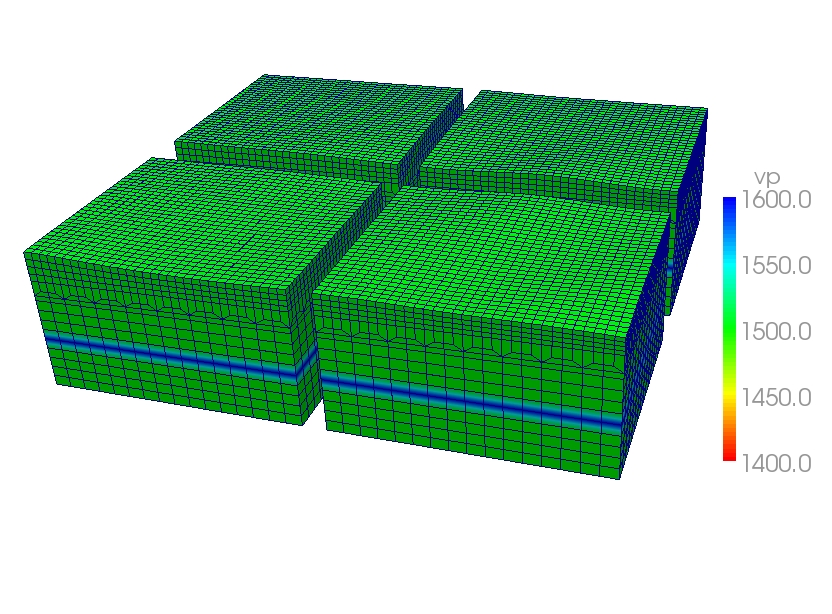
\includegraphics[width=0.49\textwidth]{figures/vtk_mesh_vp} 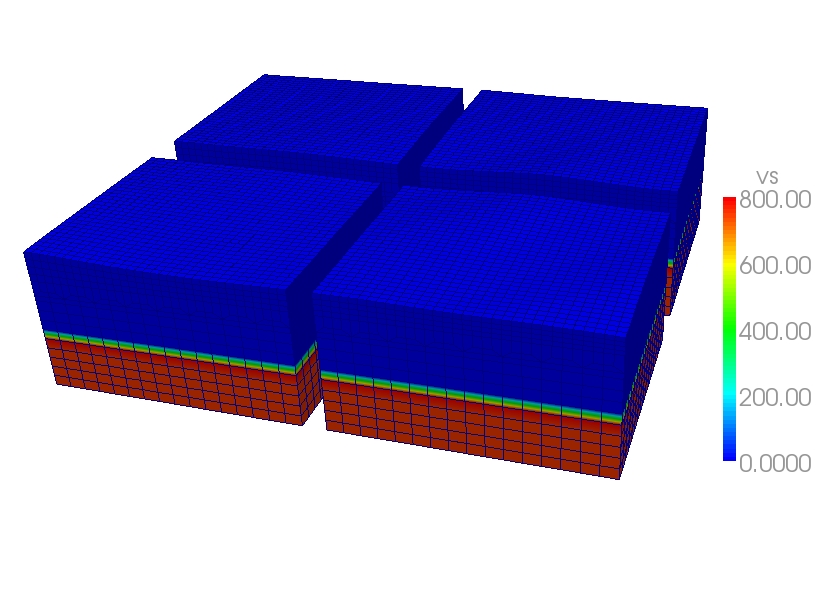
\includegraphics[width=0.49\textwidth]{figures/vtk_mesh_vs}
\par\end{centering}

\caption{Visualization using Paraview of VTK files created by \texttt{xgenerate\_databases}
showing P- and S-wave velocities assigned to the mesh points. The
mesh was created by \texttt{xmeshfem3D} for 4 processors.}


\label{fig:vtk.mesh}
\end{figure}


You have also the option to visualize the distributed databases produced
by \texttt{xgenerate\_databases} using Paraview \urlwithparentheses{www.paraview.org}.
For this, you must set the flag \texttt{SAVE\_MESH\_FILES} to \texttt{.true.}
in the main parameter file \texttt{Par\_file} (see Chapter~\ref{cha:Main-Parameter}
for details). This will create VTK files for each single partition.
You can then use Paraview \urlwithparentheses{www.paraview.org}
to visualized these partitions.


\section{\label{sec:Movies}Movies}

To make a surface or volume movie of the simulation, set parameters
\texttt{MOVIE\_SURFACE}, \texttt{MOVIE\_VOLUME}, \texttt{MOVIE\_TYPE},
and \texttt{NTSTEP\_BETWEEN\_FRAMES} in the \texttt{Par\_file}. Turning
on the movie flags, in particular \texttt{MOVIE\_VOLUME}, produces
large output files. \texttt{MOVIE\_VOLUME} files are saved in the
\texttt{LOCAL\_PATH} directory, whereas \texttt{MOVIE\_SURFACE} output
files are saved in the \texttt{OUTPUT\_FILES} directory. We save the
displacement field if the parameter \texttt{SAVE\_DISPLACEMENT} is
set, otherwise the velocity field is saved. The look of a movie is
determined by the half-duration of the source. The half-duration should
be large enough so that the movie does not contain frequencies that
are not resolved by the mesh, i.e., it should not contain numerical
noise. This can be accomplished by selecting a CMT \texttt{HALF\_DURATION}
> 1.1 $\times$ smallest period (see figure \ref{fig:CMTSOLUTION-file}).
When \texttt{MOVIE\_SURFACE} = .\texttt{true.}, the half duration
of each source in the \texttt{CMTSOLUTION} file is replaced by
\begin{quote}
\[
\sqrt{(}\mathrm{\mathtt{HALF\_DURATIO}\mathtt{N}^{2}}+\mathrm{\mathtt{HDUR\_MOVI}\mathtt{E}^{2}})
\]
 \textbf{NOTE:} If \texttt{HDUR\_MOVIE} is set to 0.0, the code will
select the appropriate value of 1.1 $\times$ smallest period. As
usual, for a point source one can set \texttt{half duration} in the
\texttt{CMTSOLUTION} file to be 0.0 and \texttt{HDUR\_MOVIE} = 0.0
in the \texttt{Par\_file} to get the highest frequencies resolved
by the simulation, but for a finite source one would keep all the
\texttt{half durations} as prescribed by the finite source model and
set \texttt{HDUR\_MOVIE} = 0.0.
\end{quote}

\subsection{Movie Surface}

When running \texttt{xspecfem3D} with the \texttt{MOVIE\_SURFACE}
flag turned on, the code outputs \texttt{moviedata??????} files in
the \texttt{OUTPUT\_FILES} directory. There are several flags in the
main parameter file \texttt{Par\_file} that control the output of
these movie data files (see section \ref{cha:Main-Parameter} for
details): \texttt{\small NTSTEP\_BETWEEN\_FRAMES}{\small{} to set the
timesteps between frames, }\texttt{\small SAVE\_DISPLACEMENT}{\small{}
to save displacement instead of velocity, }\texttt{\small USE\_HIGHRES\_FOR\_MOVIES}{\small{}
to save values at all GLL point instead of element edges. In order
to output additionally shakemaps, you would set the parameter }\texttt{\small CREATE\_SHAKEMAP}{\small{}
to }\texttt{\small .true.}{\small .}{\small \par}

The files are in a fairly complicated binary format, but there is
a program provided to convert the output into more user friendly formats:
\begin{description}
\item [{\texttt{xcreate\_movie\_shakemap\_AVS\_DX\_GMT}}] From \texttt{create\_movie\_shakemap\_AVS\_DX\_GMT.f90},
it outputs data in ASCII, OpenDX, or AVS format (also readable in
ParaView). Before compiling the code, make sure you have the file
\texttt{surface\_from\_mesher.h} in the \texttt{OUTPUT\_FILES/} directory.
This file will be created by the solver run. Then type

\begin{lyxcode}
{\footnotesize make~xcreate\_movie\_shakemap\_AVS\_DX\_GMT}{\footnotesize \par}
\end{lyxcode}

and run the executable \texttt{xcreate\_movie\_shakemap\_AVS\_DX\_GMT}
in the \texttt{bin/} subdirectory. It will create visualization files
in your format of choice. The code will prompt the user for input
parameters.


\begin{figure}[htbp]
\noindent \begin{centering}
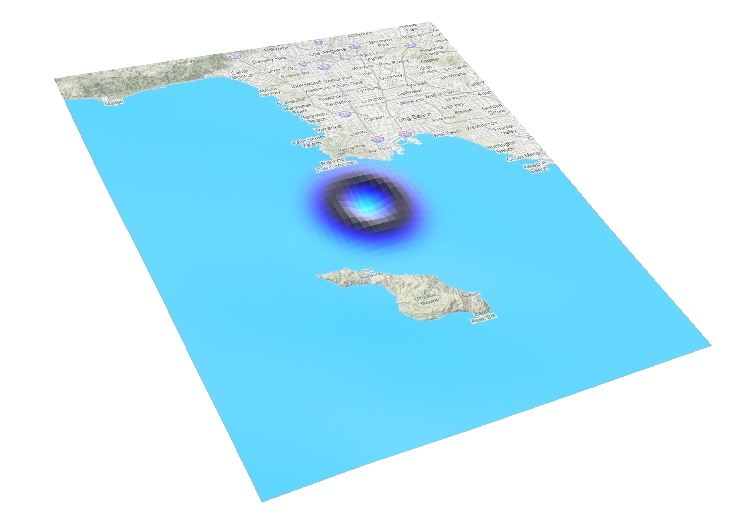
\includegraphics[width=0.32\textwidth]{figures/movie_surf_1} 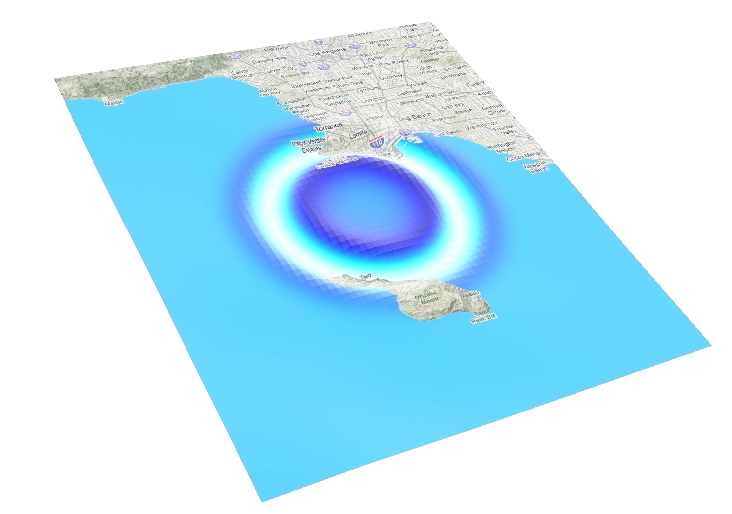
\includegraphics[width=0.32\textwidth]{figures/movie_surf_2}
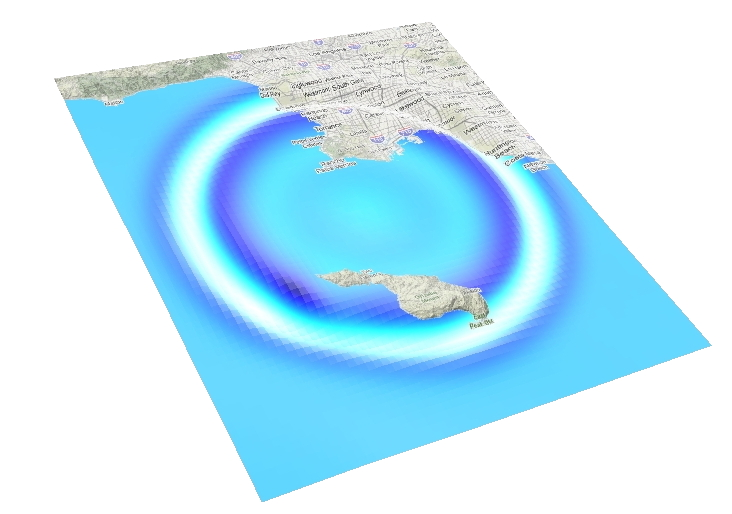
\includegraphics[width=0.32\textwidth]{figures/movie_surf_3}
\par\end{centering}

\caption{Visualization using AVS files created by \texttt{xcreate\_movie\_shakemap\_AVS\_DX\_GMT}
showing movie snapshots of vertical velocity components at different
times.}


\label{fig:movie.surf}
\end{figure}


\end{description}
The \texttt{SPECFEM3D Cartesian} code is running in near real-time
to produce animations of southern California earthquakes via the web;
see Southern California ShakeMovie\textregistered{}\urlwithparentheses{www.shakemovie.caltech.edu}.


\subsection{\label{sub:Movie-Volume}Movie Volume}

When running xspecfem3D with the \texttt{\small MOVIE\_VOLUME}{\small{}
flag turned on, the code outputs several files in }\texttt{\small LOCAL\_PATH}{\small{}
specified in the main }\texttt{\small Par\_file}{\small , e.g. in
directory }\texttt{\small OUTPUT\_FILES/DATABASES\_MPI}{\small . %As the files can be very large, there are several flags in the \texttt{\small Par\_file}
%that control the region in space and time that is saved. These are:
%\texttt{\small NTSTEP\_BETWEEN\_FRAMES}
The output is saved by each processor at the time interval specified
by }\texttt{\small NTSTEP\_BETWEEN\_FRAMES}{\small . For all domains,
the velocity field is output to files: }\texttt{\small proc??????\_velocity\_X\_it??????.bin}{\small ,
}\texttt{\small proc??????\_velocity\_Y\_it??????.bin}{\small{} and
}\texttt{\small proc??????\_velocity\_Z\_it??????.bin}{\small . For
elastic domains, the divergence and curl taken from the velocity field,
i.e. $\nabla\cdot{\bf {v}}$ and $\nabla\times{\bf {v}}$, get stored
as well: }\texttt{\small proc??????\_div\_it??????.bin}{\small , }\texttt{\small proc??????\_curl\_X\_t??????.bin}{\small ,
}\texttt{\small proc??????\_curl\_Y\_it??????.bin}{\small{} and }\texttt{\small proc??????\_curl\_Z\_it??????.bin}{\small .
The files denoted }\texttt{\small proc??????\_div\_}{\small ~}\\
{\small{} }\texttt{\small glob\_it??????.bin}{\small{} and }\texttt{\small proc??????\_curl\_glob\_it??????.bin}{\small{}
are stored on the global points only, all the other arrays are stored
on all GLL points. Note that the components X/Y/Z can change to E/N/Z
according to the }\texttt{\small SUPPRESS\_UTM\_PROJECTION}{\small{}
flag (see also Appendix~\ref{cha:Coordinates} and \ref{cha:channel-codes}).}{\small \par}

\begin{figure}[htbp]
\noindent \begin{centering}
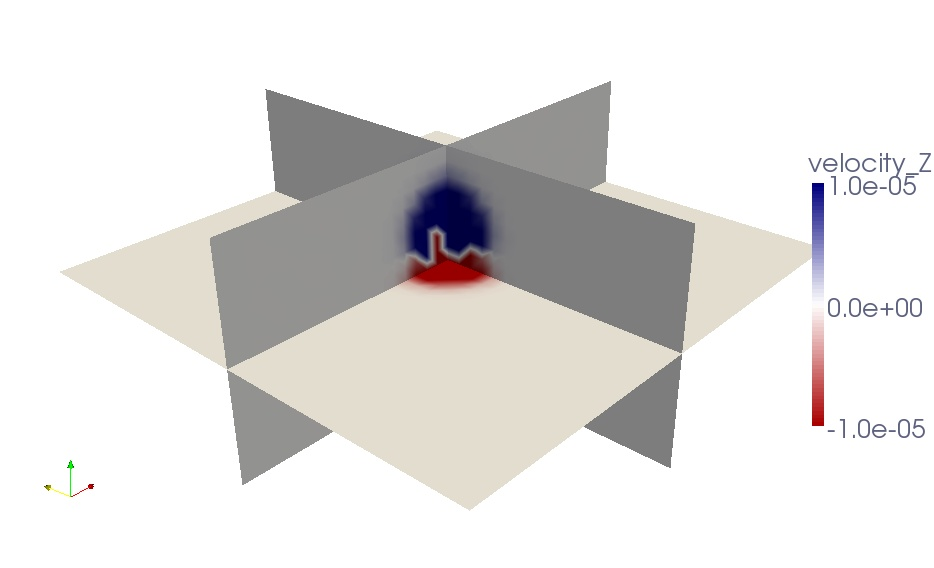
\includegraphics[width=0.32\textwidth]{figures/movie_volume_1} 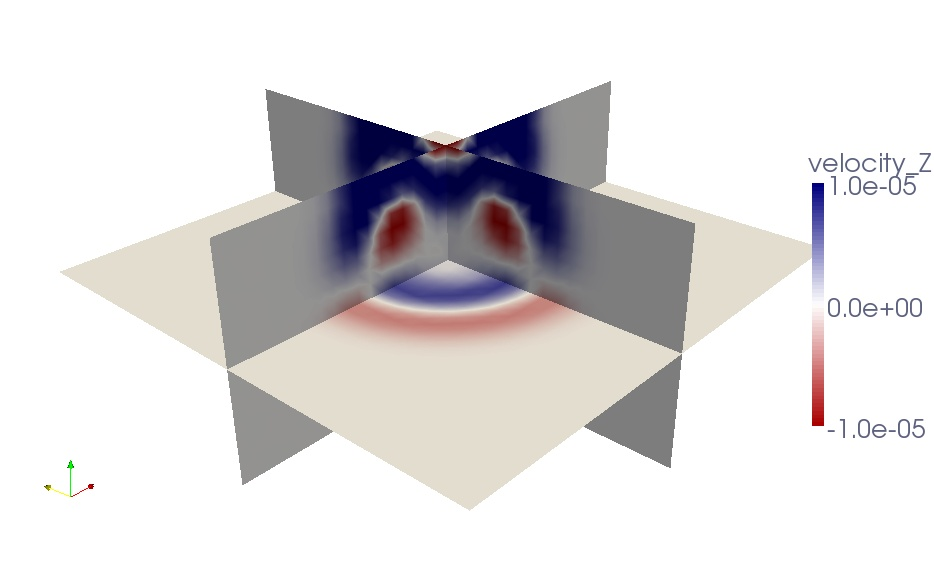
\includegraphics[width=0.32\textwidth]{figures/movie_volume_2}
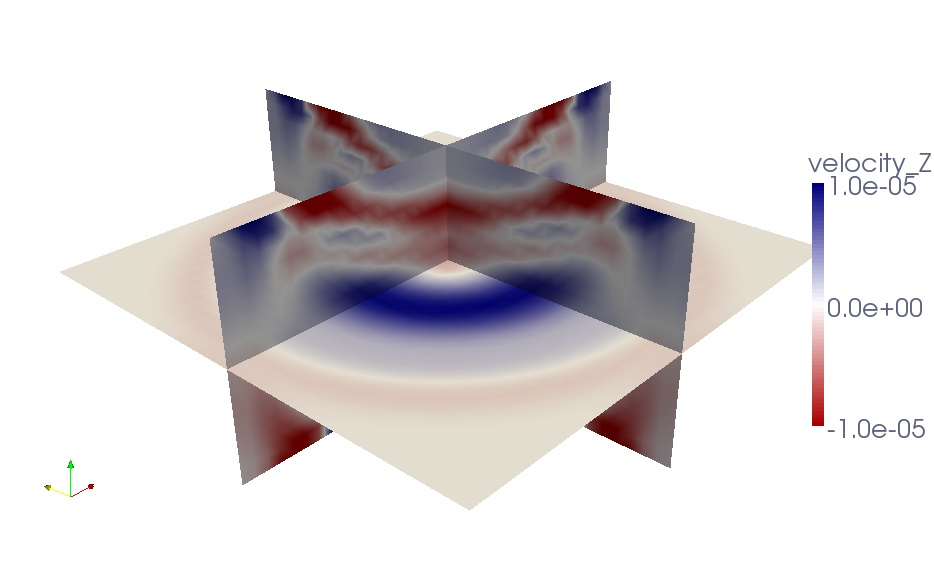
\includegraphics[width=0.32\textwidth]{figures/movie_volume_3}
\par\end{centering}

\caption{Paraview visualization using movie volume files (converted by \texttt{xcombine\_vol\_data}
and \texttt{mesh2vtu.pl}) and showing snapshots of vertical velocity
components at different times.}


\label{fig:movie.volume}
\end{figure}


To visualize these files, we use an auxilliary program \texttt{combine\_vol\_data.f90}
to combine the data from all slices into one mesh file. To compile
it in the root directory, type:
\begin{lyxcode}
{\footnotesize make~xcombine\_vol\_data~}{\footnotesize \par}
\end{lyxcode}
which will create the executable \texttt{xcombine\_vol\_data} in the
directory \texttt{bin/}. To output the usage of this executable, type
`./bin/xcombine\_vol\_data` without arguments. As an example, to run
the executable you would use
\begin{lyxcode}
{\footnotesize cd~bin/~}{\footnotesize \par}

~{\footnotesize ./xcombine\_vol\_data~0~3~velocity\_Z\_it000400~../OUTPUT\_FILES/DATABASES\_MPI~../OUTPUT\_FILES~0~}{\footnotesize \par}
\end{lyxcode}
to create a low-resolution mesh file. The output mesh file will have
the name \texttt{velocity\_Z\_it000400.mesh}. We next convert the
\texttt{.mesh} file into the VTU (Unstructured grid file) format which
can be viewed in ParaView. For this task, you can use and modify the
script \texttt{mesh2vtu.pl} located in directory \texttt{utils/Visualization/Paraview/},
for example:
\begin{lyxcode}
{\footnotesize mesh2vtu.pl~-i~velocity\_Z\_it000400.mesh~-o~velocity\_Z\_it000400.vtu}{\footnotesize \par}
\end{lyxcode}
Notice that this Perl script uses a program \texttt{mesh2vtu} in the
\texttt{utils/Visualization/Paraview/mesh2vtu} directory, which further
uses the VTK \urlwithparentheses{http://www.vtk.org/} run-time library
for its execution. Therefore, make sure you have them properly set
in the script according to your system.


\section{\label{sec:Finite-Frequency-Kernels}Finite-Frequency Kernels}

The finite-frequency kernels computed as explained in Section \ref{sec:Adjoint-simulation-finite}
are saved in the \texttt{LOCAL\_PATH} at the end of the simulation.
Therefore, we first need to collect these files on the front end,
combine them into one mesh file, and visualize them with some auxilliary
programs.
\begin{enumerate}
\item \textbf{Create slice files}


We will only discuss the case of one source-receiver pair, i.e., the
so-called banana-doughnut kernels. Although it is possible to collect
the kernel files from all slices on the front end, it usually takes
up too much storage space (at least tens of gigabytes). Since the
sensitivity kernels are the strongest along the source-receiver great
circle path, it is sufficient to collect only the slices that are
along or close to the great circle path.


A Perl script \texttt{slice\_number.pl} located in directory \texttt{utils/Visualization/Paraview/}
can help to figure out the slice numbers that lie along the great
circle path. It applies to meshes created with the internal mesher
\texttt{xmeshfem3D}.
\begin{enumerate}
\item On machines where you have access to the script, copy the \texttt{Mesh\_Par\_file},
and \texttt{output\_solver} files, and run:

\begin{lyxcode}
{\small slice\_number.pl~Mesh\_Par\_file~output\_solver.txt~slice\_file}{\small \par}
\end{lyxcode}

which will generate a \texttt{slices\_file}.

\item For cases with multiple sources and multiple receivers, you need to
provide a slice file before proceeding to the next step.
\end{enumerate}
\item \textbf{Collect the kernel files}


After obtaining the slice files, you can collect the corresponding
kernel files from the given slices.
\begin{enumerate}
\item You can use or modify the script \texttt{utils/copy\_basin\_database.pl}
to accomplish this:

\begin{lyxcode}
{\small utils/copy\_database.pl~slice\_file~lsf\_machine\_file~filename~{[}jobid{]}}{\small \par}
\end{lyxcode}

where \texttt{\small lsf\_machine\_file}{\small{} is the machine file
generated by the LSF scheduler, }\texttt{\small filename}{\small{}
is the kernel name (e.g., }\texttt{\small rho\_kernel}{\small , }\texttt{\small alpha\_kernel}{\small{}
and }\texttt{\small beta\_kernel}{\small ), and the optional }\texttt{\small jobid}{\small{}
is the name of the subdirectory under }\texttt{\small LOCAL\_PATH}{\small{}
where all the kernel files are stored.}{\small \par}

\item After executing this script, all the necessary mesh topology files
as well as the kernel array files are collected to the local directory
of the front end.
\end{enumerate}
\item \textbf{Combine kernel files into one mesh file}


We use an auxilliary program \texttt{combine\_vol\_data.f90} to combine
the kernel files from all slices into one mesh file.
\begin{enumerate}
\item Compile it in the root directory:

\begin{lyxcode}
{\footnotesize make~xcombine\_vol\_data~}{\footnotesize \par}

{\footnotesize ./bin/xcombine\_vol\_data~slice\_list~filename~input\_dir~output\_dir~high/low-resolution~}{\footnotesize \par}
\end{lyxcode}

where \texttt{input\_dir} is the directory where all the individual
kernel files are stored, and \texttt{output\_dir} is where the mesh
file will be written.

\item Use 1 for a high-resolution mesh, outputting all the GLL points to
the mesh file, or use 0 for low resolution, outputting only the corner
points of the elements to the mesh file.
\item The output mesh file will have the name \texttt{filename\_rho(alpha,beta).mesh}
\end{enumerate}
\item \textbf{Convert mesh files into .vtu files}

\begin{enumerate}
\item We next convert the \texttt{.mesh} file into the VTU (Unstructured
grid file) format which can be viewed in ParaView. For this task,
you can use and modify the script \texttt{mesh2vtu.pl} located in
directory \texttt{utils/Visualization/Paraview/}, for example:

\begin{lyxcode}
{\footnotesize mesh2vtu.pl~-i~file.mesh~-o~file.vtu~}{\footnotesize \par}
\end{lyxcode}
\item Notice that this Perl script uses a program \texttt{mesh2vtu} in the
\texttt{utils/Visualization/Paraview/mesh2vtu} directory, which further
uses the VTK \urlwithparentheses{http://www.vtk.org/} run-time library
for its execution. Therefore, make sure you have them properly set
in the script according to your system.
\end{enumerate}
\item \textbf{Copy over the source and receiver .vtk file}


In the case of a single source and a single receiver, the simulation
also generates the file \texttt{sr.vtk} located in the \texttt{OUTPUT\_FILES/}
directory to describe the source and receiver locations, which can
also be viewed in Paraview in the next step.

\item \textbf{View the mesh in ParaView}


Finally, we can view the mesh in ParaView \urlwithparentheses{www.paraview.org}.
\begin{enumerate}
\item Open ParaView.
\item From the top menu, \textsf{File} $\rightarrow$\textsf{Open data},
select \texttt{file.vtu}, and click the \textsf{Accept} button.

\begin{itemize}
\item If the mesh file is of moderate size, it shows up on the screen; otherwise,
only the bounding box is shown.
\end{itemize}
\item Click \textsf{Display Tab} $\rightarrow$ \textsf{Display Style} $\rightarrow$
\textsf{Representation} and select \textsf{wireframe of surface} to
display it.
\item To create a cross-section of the volumetric mesh, choose \textsf{Filter}
$\rightarrow$ \textsf{cut}, and under \textsf{Parameters Tab}, choose
\textsf{Cut Function} $\rightarrow$ \textsf{plane}.
\item Fill in center and normal information given by the \texttt{global\_slice\_number.pl}
script (either from the standard output or from \texttt{normal\_plane.txt}
file).
\item To change the color scale, go to \textsf{Display Tab} $\rightarrow$
\textsf{Color} $\rightarrow$ \textsf{Edit Color Map} and reselect
lower and upper limits, or change the color scheme.
\item Now load in the source and receiver location file by \textsf{File}
$\rightarrow$ \textsf{Open data}, select \texttt{sr.vt}k, and click
the \textsf{Accept} button. Choose \textsf{Filter} $\rightarrow$
\textsf{Glyph}, and represent the points by `\textsf{spheres}'.
\item For more information about ParaView, see the ParaView Users Guide
\urlwithparentheses{www.paraview.org/files/v1.6/ParaViewUsersGuide.PDF}.
\end{enumerate}
\end{enumerate}
\begin{figure}[H]
\noindent \begin{centering}
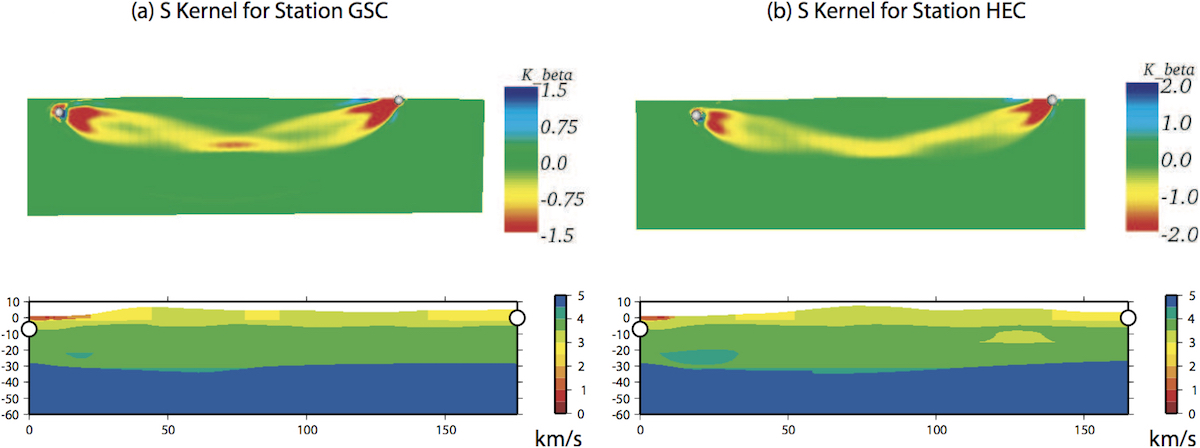
\includegraphics[scale=0.6]{figures/3D-S-Kernel}
\par\end{centering}

\caption{(a) Top Panel: Vertical source-receiver cross-section of the S-wave
finite-frequency sensitivity kernel $K_{\beta}$ for station GSC at
an epicentral distance of 176 km from the September 3, 2002, Yorba
Linda earthquake. Lower Panel: Vertical source-receiver cross-section
of the 3D S-wave speed model used for the spectral-element simulations
\citep{KoLiTrSuStSh04}. (b) The same as (a) but for station HEC at
an epicentral distance of 165 km \citep{LiTr06}.}


\label{figure:P-wave-speed-finite-frequency}
\end{figure}



\chapter{\label{cha:Scheduler}Running through a Scheduler}

The code is usually run on large parallel machines, often PC clusters,
most of which use schedulers, i.e., queuing or batch management systems
to manage the running of jobs from a large number of users. The following
considerations need to be taken into account when running on a system
that uses a scheduler:
\begin{itemize}
\item The processors/nodes to be used for each run are assigned dynamically
by the scheduler, based on availability. Therefore, in order for the
\texttt{xgenerate\_databases} and the \texttt{xspecfem3D} executables
(or between successive runs of the solver) to have access to the same
database files (if they are stored on hard drives local to the nodes
on which the code is run), they must be launched in sequence as a
single job.
\item On some systems, the nodes to which running jobs are assigned are
not configured for compilation. It may therefore be necessary to pre-compile
both the \texttt{xgenerate\_databases} and the \texttt{xspecfem3D}
executables.
\item One feature of schedulers/queuing systems is that they allow submission
of multiple jobs in a ``launch and forget'' mode. In order to take
advantage of this property, care needs to be taken that output and
intermediate files from separate jobs do not overwrite each other,
or otherwise interfere with other running jobs.
\end{itemize}
Examples of job scripts can be found in the \texttt{\small utils/Cluster/}{\small{}
directory and can straightforwardly be modified and adapted to meet
more specific running needs.}{\small \par}

We describe here in some detail a job submission procedure for the
Caltech 1024-node cluster, CITerra, under the LSF scheduling system.
We consider the submission of a regular forward simulation using the
internal mesher to create mesh partitions. The two main scripts are
\texttt{\small run\_lsf.bash}{\small , which compiles the Fortran
code and submits the job to the scheduler, and }\texttt{\small go\_mesher\_solver\_lsf\_basin.forward}{\small ,
which contains the instructions that make up the job itself. These
scripts can be found in }\texttt{\small utils/Cluster/lsf/}{\small{}
directory}{\small \par}


\section{Job submission \texttt{run\_lsf.bash}}

This script first sets the job queue to be `normal'. It then compiles
the mesher, database generator and solver together, figures out the
number of processors required for this simulation from the \texttt{DATA/Par\_file},
and submits the LSF job.
\begin{lyxcode}
\#!/bin/bash

\#~use~the~normal~queue~unless~otherwise~directed~queue=\textquotedbl{}-q~normal\textquotedbl{}~

if~{[}~\$\#~-eq~1~{]};~then

~~~~~~~~echo~\textquotedbl{}Setting~the~queue~to~\$1\textquotedbl{}

~~~~~~~~queue=\textquotedbl{}-q~\$1\textquotedbl{}~

fi~~\\
~~~\\
~\#~compile~the~mesher~and~the~solver~

d=`date'~echo~\textquotedbl{}Starting~compilation~\$d\textquotedbl{}~

make~clean~

make~xmeshfem3D~

make~xgenerate\_databases~

make~xspecfem3D~

d=`date'~

echo~\textquotedbl{}Finished~compilation~\$d\textquotedbl{}~~\\
~~~\\
~\#~get~total~number~of~nodes~needed~for~solver~

NPROC=`grep~NPROC~DATA/Par\_file~|~cut~-c~34-~'~~\\
~~~\\


\#~compute~total~number~of~nodes~needed~for~mesher~

NPROC\_XI=`grep~NPROC\_XI~DATA/meshfem3D\_files/Mesh\_Par\_file~|~cut~-c~34-~'~~~~\\


NPROC\_ETA=`grep~NPROC\_ETA~DATA/meshfem3D\_files/Mesh\_Par\_file~|~cut~-c~34-~'~~~~\\
~\#~total~number~of~nodes~is~the~product~of~the~values~read~

numnodes=\$((~\$NPROC\_XI~{*}~\$NPROC\_ETA~))~~\\
~~~\\


\#~checks~total~number~of~nodes~

if~{[}~\$numnodes~-neq~\$NPROC~{]};~then

~~~~~~~~echo~\textquotedbl{}error~number~of~procs~mismatch\textquotedbl{}

~~~~~~~~exit~

fi~~\\


~~\\
~echo~\textquotedbl{}Submitting~job\textquotedbl{}~

bsub~\$queue~-n~\$numnodes~-W~60~-K~<go\_mesher\_solver\_lsf.forward~
\end{lyxcode}

\section{Job script \texttt{go\_mesher\_solver\_lsf.forward}}

This script describes the job itself, including setup steps that can
only be done once the scheduler has assigned a job-ID and a set of
compute nodes to the job, the \texttt{run\_lsf.bash} commands used
to run the mesher, database generator and the solver, and calls to
scripts that collect the output seismograms from the compute nodes
and perform clean-up operations.
\begin{enumerate}
\item First the script directs the scheduler to save its own output and
output from \texttt{stdout} into ~\\
 \texttt{\small OUTPUT\_FILES/\%J.o}{\small , where }\texttt{\small \%J}{\small{}
is short-hand for the job-ID; it also tells the scheduler what version
of }\texttt{\small mpich}{\small{} to use (}\texttt{\small mpich\_gm}{\small )
and how to name this job (}\texttt{\small go\_mesher\_solver\_lsf}{\small ). }{\small \par}
\item The script then creates a list of the nodes allocated to this job
by echoing the value of a dynamically set environment variable \texttt{LSB\_MCPU\_HOSTS}
and parsing the output into a one-column list using the Perl script
\texttt{utils/Cluster/lsf/remap\_lsf\_machines.pl}. It then creates
a set of scratch directories on these nodes (\texttt{\small /scratch/}{\small ~}\\
{\small{} }\texttt{\small \$USER/DATABASES\_MPI}{\small ) to be used
as the }\texttt{\small LOCAL\_PATH}{\small{} for temporary storage
of the database files. The scratch directories are created using }\texttt{\small shmux}{\small ,
a shell multiplexor that can execute the same commands on many hosts
in parallel. }\texttt{\small shmux}{\small{} is available from Shmux
\urlwithparentheses{web.taranis.org/shmux/}. Make sure that the
}\texttt{\small LOCAL\_PATH}{\small{} parameter in }\texttt{\small DATA/Par\_file}{\small{}
is also set properly. }{\small \par}
\item The next portion of the script launches the mesher, database generator
and then the solver using \texttt{run\_lsf.bash}.
\item The final portion of the script collects the seismograms and performs
clean up on the nodes, using the Perl scripts \texttt{collect\_seismo\_lsf\_multi.pl}
and \texttt{cleanmulti.pl}. \end{enumerate}
\begin{lyxcode}
\#!/bin/bash~-v~

\#BSUB~-o~OUTPUT\_FILES/\%J.o~

\#BSUB~-a~mpich\_gm~

\#BSUB~-J~go\_mesher\_solver\_lsf~~\\
~~~\\
~\#~set~up~local~scratch~directories

BASEMPIDIR=/scratch/\$USER/DATABASES\_MPI

mkdir~-p~OUTPUT\_FILES~

echo~\textquotedbl{}\$LSB\_MCPU\_HOSTS\textquotedbl{}~>~OUTPUT\_FILES/lsf\_machines~

echo~\textquotedbl{}\$LSB\_JOBID\textquotedbl{}~>~OUTPUT\_FILES/jobid

remap\_lsf\_machines.pl~OUTPUT\_FILES/lsf\_machines~>~OUTPUT\_FILES/machines

shmux~-M50~-Sall~-c~\textquotedbl{}rm~-r~-f~/scratch/\$USER;~\textbackslash{}

~~~~~~mkdir~-p~/scratch/\$USER;~mkdir~-p~\$BASEMPIDIR\textquotedbl{}~\textbackslash{}

~~~~~~-~<~OUTPUT\_FILES/machines~>/dev/null~~\\
~~~\\
~\#~run~the~specfem~program

current\_pwd=\$PWD~~\\


cd~bin/~~\\


run\_lsf.bash~-{}-gm-no-shmem~-{}-gm-copy-env~\$current\_pwd/xmeshfem3D~~\\


run\_lsf.bash~-{}-gm-no-shmem~-{}-gm-copy-env~\$current\_pwd/xgenerate\_databases~~\\


run\_lsf.bash~-{}-gm-no-shmem~-{}-gm-copy-env~\$current\_pwd/xspecfem3D~~\\
~~~\\
~\#~collect~seismograms~and~clean~up

cd~current\_pwd/~~~\\


mkdir~-p~SEM

cd~SEM/~

collect\_seismo.pl~../OUTPUT\_FILES/lsf\_machines

cleanbase.pl~../OUTPUT\_FILES/machines
\end{lyxcode}

\chapter{{\normalsize \label{cha:-Changing-the}} Changing the Model}

In this section we explain how to change the velocity model used for
your simulations. These changes involve contributing specific subroutines
that replace existing subroutines in the \texttt{SPECFEM3D Cartesian}
package. Note that \texttt{SPECFEM3D Cartesian} can handle Earth models
with material properties that vary within each spectral element.

%% magnoni 6/12



\section{{\normalsize \label{sec:Using-tomographic}}Using external tomographic
Earth models}

To implement your own external tomographic model(s), you must provide
your own external tomography file(s), and choose between two possible
options:\\
 \indent (1) set in the \texttt{Par\_file} the model parameter \texttt{MODEL
= tomo}, \\
 or for more user control: \\
 \indent (2) set in the \texttt{Par\_file} the model parameter \texttt{MODEL
= default}, define the negative \texttt{material\_ID} identifier for
each element in the file \texttt{MESH/materials\_file} and use the
following format in the file \texttt{MESH/nummaterial\_velocity\_file}
when using CUBIT to construct your mesh (see also section \ref{subsec:Exporting-the-Mesh}):
\begin{lyxcode}
domain\_ID~material\_ID~tomography~elastic~file\_name~1
\end{lyxcode}
where: \\
 \indent \texttt{domain\_ID} is 1 for acoustic or 2 for elastic materials,
\\
 \indent \texttt{material\_ID} a negative, unique identifier (i.e.,
-1,-2,...), \\
 \indent \texttt{tomography} keyword for tomographic material definition,
\\
 \indent \texttt{elastic} keyword for elastic material definition,
\\
 \indent \texttt{file\_name} the name of the tomography file and
1 a positive unique identifier.\\


The external tomographic model is represented by a grid of points
with assigned material properties and homogeneous resolution along
each spatial direction x, y and z. The ASCII file \texttt{file\_name}
that describe the tomography should be located in the \texttt{TOMOGRAPHY\_PATH}
directory, set in the \texttt{Par\_file}. The format of the file,
as read from \texttt{model\_tomography.f90} located in the \texttt{src/generate\_databases}
directory, looks like Figure \ref{fig:tomography_file}, where
\begin{description}
\item [{\texttt{ORIG\_X}, \texttt{END\_X}}] are, respectively, the coordinates
of the initial and final tomographic grid points along the x direction
(in the mesh units, e.g., $m$);
\item [{\texttt{ORIG\_Y}, \texttt{END\_Y}}] respectively the coordinates
of the initial and final tomographic grid points along the y direction
(in the mesh units, e.g., $m$);
\item [{\texttt{ORIG\_Z}, \texttt{END\_Z}}] respectively the coordinates
of the initial and final tomographic grid points along the z direction
(in the mesh units, e.g., $m$);
\item [{\texttt{SPACING\_X}, \texttt{SPACING\_Y}, \texttt{SPACING\_Z}}] the
spacing between the tomographic grid points along the x, y and z directions,
respectively (in the mesh units, e.g., $m$);
\item [{\texttt{NX}, \texttt{NY}, \texttt{NZ}}] the number of grid points
along the spatial directions x, y and z, respectively; \texttt{NX}
is given by {[}(\texttt{END\_X} - \texttt{ORIG\_X})/\texttt{SPACING\_X}{]}+1;
\texttt{NY} and \texttt{NZ} are the same as \texttt{NX}, but for the
y and z directions, respectively;
\item [{\texttt{VP\_MIN}, \texttt{VP\_MAX}, \texttt{VS\_MIN}, \texttt{VS\_MAX}, \texttt{RHO\_MIN}, \texttt{RHO\_MAX}}] the
minimum and maximum values of the wave speed \texttt{vp} and \texttt{vs}
(in $m\, s^{-1}$) and of the density \texttt{rho} (in $kg\, m^{-3}$);
these values could be the actual limits of the tomographic parameters
in the grid or the minimum and maximum values to which we force the
cut of velocity and density in the model.
\end{description}
After the first four lines, in the file \texttt{file\_name} the tomographic
grid points are listed with the corresponding values of \texttt{vp},
\texttt{vs} and \texttt{rho}, scanning the grid along the x coordinate
(from \texttt{ORIG\_X} to \texttt{END\_X} with step of \texttt{SPACING\_X})
for each given y (from \texttt{ORIG\_Y} to \texttt{END\_Y}, with step
of \texttt{SPACING\_Y}) and each given z (from \texttt{ORIG\_Z} to
\texttt{END\_Z}, with step of \texttt{SPACING\_Z}). %fig
\begin{figure}[htbp]
\noindent \begin{centering}
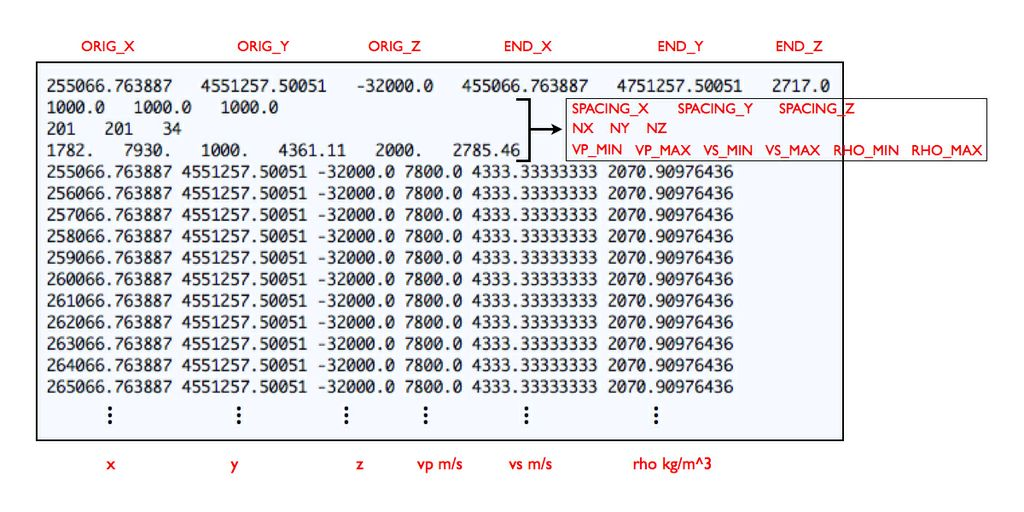
\includegraphics[width=1\textwidth]{figures/tomo_file}
\par\end{centering}

\caption{Tomography file \texttt{file\_name} that describes an external Earth
model. The coordinates x, y and z of the grid, their limits ORIG\_X,
ORIG\_Y, ORIG\_Z, END\_X, END\_Y, END\_Z and the grid spacings SPACING\_X,
SPACING\_Y, SPACING\_Z should be in the units of the constructed mesh
(e.g., UTM coordinates in meters).}


\label{fig:tomography_file}
\end{figure}


The user can implement his own interpolation algorithm for the tomography
model by changing the routine \texttt{model\_tomography.f90} located
in the \texttt{src/generate\_databases/} directory. Moreover, for
models that involve both fully defined materials and a tomography
description, the \texttt{nummaterial\_velocity\_file} has multiple
lines each with the corresponding suitable format described above.

%==============

\subsubsection*{Example: External tomography file with variable discretization intervals}

The example in Figure~\ref{fig:tomography_file} is for an external tomography file with uniform spacing in the $x$, $y$, and $z$ directions. (Note that $\Delta x$, $\Delta y$, and $\Delta z$ need not be the same as in the example.) In that example, the  \texttt{nummaterial\_velocity\_file} is
%
\begin{lyxcode}
2  -1 tomography elastic tomography\_model.xyz 1
\end{lyxcode}
%
and the file \texttt{tomography\_model.xyz} will need to reside in \texttt{DATA/}. All entries in the second column of \texttt{materials\_file} will be \texttt{-1}, which means that each element in the mesh will be interpolated accordind to the values in \texttt{tomography\_model.xyz}.

In some cases it may be desirable to have an external tomography model that is described in more than one file. For example, in cases like southern California, the length scale of variation in the structure of the wave speed model is much shorter in the sedimentary basin models within the upper 15~km. Therefore one might want to use an external tomography file that is sampled with, say, $\Delta x = 1000$~m, $\Delta y = 1000$~m, and $\Delta z = 250$~m in the uppermost 15~km, and then use $\Delta x = 2000$~m, $\Delta y = 2000$~m, and $\Delta z = 1000$~m below a depth of 15~km. If these intervals are chosen appropriately, then it will result in a pair of external tomography file that is much smaller than the alternative of having a single file with the fine discretization. In this case  \texttt{nummaterial\_velocity\_file} is
%
\begin{lyxcode}
2  -1 tomography elastic file\_above\_15km.xyz 1 \\
2  -2 tomography elastic file\_below\_15km.xyz 1
\end{lyxcode}
%
and the files \texttt{file\_above\_15km.xyz} and \texttt{file\_below\_15km.xyz} will need to reside in \texttt{DATA/}.  All entries in the second column of \texttt{materials\_file} will need to be either \texttt{-1} or \texttt{-2}, depending on whether the element is above or below 15~km depth. In this sense, the construction of the mesh and the discretization of the external model will generally be done in tandem.

Other more complicated discretizations can be used following the same procedure. (In particular, there is no limit on the number of different external files that are used.)

%=============

\section{{\normalsize \label{sec:Anelastic-Models}}External (an)elastic Models}

To use your own external model, you can set in the \texttt{Par\_file}
the model parameter \texttt{MODEL = external}. Three-dimensional acoustic
and/or (an)elastic (attenuation) models may then be superimposed onto
the mesh based upon your subroutine in \texttt{model\_external\_values.f90}
located in directory \texttt{src/generate\_databases}. The call to
this routine would be as follows
\begin{lyxcode}
call~model\_external\_values(xmesh,~ymesh,~zmesh,~~\&~~\\
~~~~~~~~~~~rho,~vp,~vs,~qmu\_atten,~iflag\_aniso,~idomain\_id)
\end{lyxcode}
Input to this routine consists of:
\begin{description}
\item [{\texttt{xmesh,ymesh,zmesh}}] location of mesh point
\end{description}
Output to this routine consists of:
\begin{description}
\item [{\texttt{rho,vp,vs}}] isotropic model parameters for density $\rho$
($kg/m^{3}$), $v_{p}$ ($m/s$) and $v_{s}$ ($m/s$)
\item [{\texttt{qmu\_atten}}] Shear wave quality factor: $0<Q_{\mu}<9000$
\item [{\texttt{iflag\_aniso}}] anisotropic model flag, $0$ indicating
no anisotropy or $1$ using anisotropic model parameters as defined
in routine file \texttt{model\_aniso.f90}
\item [{\texttt{idomain\_id}}] domain identifier, $1$ for acoustic, $2$
for elastic, $3$ for poroelastic materials.
\end{description}
Note that the resolution and maximum value of anelastic models are
truncated. This speeds the construction of the standard linear solids
during the meshing stage. To change the resolution, currently at one
significant figure following the decimal, or the maximum value (9000),
consult \texttt{shared/constants.h}.


\section{{\normalsize \label{sec:Anisotropic-Models}}Anisotropic Models}

To use your anisotropic models, you can either set in the \texttt{Par\_file}
the model parameter \texttt{ANISOTROPY} to \texttt{.true.} or set
the model parameter \texttt{MODEL = aniso}. Three-dimensional anisotropic
models may be superimposed on the mesh based upon the subroutine in
file \texttt{model\_aniso.f90} located in directory \texttt{src/generate\_databases}.
The call to this subroutine is of the form
\begin{lyxcode}
call~model\_aniso(iflag\_aniso,~rho,~vp,~vs,~\&~~\\
~~~~~~~~~~~c11,c12,c13,c14,c15,c16,c22,c23,c24,c25,c26,~\&~~\\
~~~~~~~~~~~c33,c34,c35,c36,c44,c45,c46,c55,c56,c66)~
\end{lyxcode}
Input to this routine consists of:
\begin{description}
\item [{\texttt{iflag\_aniso}}] flag indicating the type of the anisotropic
model, i.e. $0$ for no superimposed anisotropy, $1$ or $2$ for
generic pre-defined anisotropic models.
\item [{\texttt{rho,vp,vs}}] reference isotropic model parameters for density
$\rho$, $v_{p}$ and $v_{s}$.
\end{description}
Output from the routine consists of the following non-dimensional
model parameters:
\begin{description}
\item [{\texttt{c11},}] \textbf{$\cdots$,} \texttt{\textbf{c66}} 21~dimensionalized
anisotropic elastic parameters.
\end{description}
You can replace the \texttt{model\_aniso.f90} file by your own version
\textit{provided you do not change the call structure of the routine},
i.e., the new routine should take exactly the same input and produce
the required relative output.


\chapter{Post-Processing Scripts}

Several post-processing scripts/programs are provided in the \texttt{utils/}
directory, and most of them need to be adjusted when used on different
systems, for example, the path of the executable programs. Here we
only list a few of the available scripts and provide a brief description,
and you can either refer to the related sections for detailed usage
or, in a lot of cases, type the script/program name without arguments
for its usage.


\section{Process Data and Synthetics\label{sec:Process-data-and-syn}}

In many cases, the SEM synthetics are calculated and compared to data
seismograms recorded at seismic stations. Since the SEM synthetics
are accurate for a certain frequency range, both the original data
and the synthetics need to be processed before a comparison can be
made.

For such comparisons, the following steps are recommended:
\begin{enumerate}
\item Make sure that both synthetic and observed seismograms have the correct
station/event and timing information.
\item Convolve synthetic seismograms with a source time function with the
half duration specified in the \texttt{CMTSOLUTION} file, provided,
as recommended, you used a zero half duration in the SEM simulations.
\item Resample both observed and synthetic seismograms to a common sampling
rate.
\item Cut the records using the same window.
\item Remove the trend and mean from the records and taper them.
\item Remove the instrument response from the observed seismograms (recommended)
or convolve the synthetic seismograms with the instrument response.
\item Make sure that you apply the same filters to both observed and synthetic
seismograms. Preferably, avoid filtering your records more than once.
\item Now, you are ready to compare your synthetic and observed seismograms.
\end{enumerate}
\noindent We generally use the following scripts provided in the \texttt{utils/seis\_process/}
directory:


\subsection{Data processing script \texttt{process\_data.pl}}

This script cuts a given portion of the original data, filters it,
transfers the data into a displacement record, and picks the first
P and S arrivals. For more functionality, type `\texttt{process\_data.pl}'
without any argument. An example of the usage of the script:
\begin{lyxcode}
{\footnotesize process\_data.pl~-m~CMTSOLUTION~-s~1.0~-l~0/4000~-i~-f~-t~40/500~-p~-x~bp~DATA/1999.330{*}.BH?.SAC}~
\end{lyxcode}
\noindent which has resampled the SAC files to a sampling rate of
1 seconds, cut them between 0 and 4000 seconds, transfered them into
displacement records and filtered them between 40 and 500 seconds,
picked the first P and S arrivals, and added suffix `\texttt{bp}'
to the file names.

Note that all of the scripts in this section actually use the SAC
and/or IASP91 to do the core operations; therefore make sure that
the SAC and IASP91 packages are installed properly on your system,
and that all the environment variables are set properly before running
these scripts.


\subsection{Synthetics processing script \texttt{process\_syn.pl}}

This script converts the synthetic output from the SEM code from ASCII
to SAC format, and performs similar operations as `\texttt{process\_data.pl}'.
An example of the usage of the script:
\begin{lyxcode}
{\footnotesize process\_syn.pl~-m~CMTSOLUTION~-h~-a~STATIONS~-s~1.0~-l~0/4000~-f~-t~40/500~-p~-x~bp~SEM/{*}.BX?.semd}~
\end{lyxcode}
which will convolve the synthetics with a triangular source-time function
from the \texttt{CMTSOLUTION} file, convert the synthetics into SAC
format, add event and station information into the SAC headers, resample
the SAC files with a sampling rate of 1 seconds, cut them between
0 and 4000 seconds, filter them between 40 and 500 seconds with the
same filter used for the observed data, pick the first P and S arrivals,
and add the suffix `\texttt{bp}' to the file names.

More options are available for this script, such as adding time shift
to the origin time of the synthetics, convolving the synthetics with
a triangular source time function with a given half duration, etc.
Type \texttt{process\_syn.pl} without any argument for a detailed
usage.

In order to convert between SAC format and ASCII files, useful scripts
are provided in the subdirectories ~\\
 \texttt{utils/sac2000\_alpha\_convert/} and \texttt{utils/seis\_process/asc2sac/}.


\subsection{Script \texttt{rotate.pl}}

The original data and synthetics have three components: vertical (BHZ
resp. BXZ), north (BHN resp. BXN) and east (BHE resp. BXE). However,
for most seismology applications, transverse and radial components
are also desirable. Therefore, we need to rotate the horizontal components
of both the data and the synthetics to the transverse and radial direction,
and \texttt{\small rotate.pl}{\small{} can be used to accomplish this:}{\small \par}
\begin{lyxcode}
rotate.pl~-l~0~-L~180~-d~DATA/{*}.BHE.SAC.bp~

rotate.pl~-l~0~-L~180~SEM/{*}.BXE.semd.sac.bp~
\end{lyxcode}
where the first command performs rotation on the SAC data obtained
through Seismogram Transfer Program (STP) \urlwithparentheses{http://www.data.scec.org/STP/stp.html},
while the second command rotates the processed SEM synthetics.


\section{Collect Synthetic Seismograms}

The forward and adjoint simulations generate synthetic seismograms
in the \texttt{OUTPUT\_FILES/} directory by default. For the forward
simulation, the files are named like \texttt{STA.NT.BX?.semd} for
two-column time series, or \texttt{STA.NT.BX?.semd.sac} for ASCII
SAC format, where STA and NT are the station name and network code,
and \texttt{BX?} stands for the component name. Please see the Appendix~\ref{cha:Coordinates}
and \ref{cha:channel-codes} for further details.

The adjont simulations generate synthetic seismograms with the name
\texttt{S?????.NT.S??.sem} (refer to Section \ref{sec:Adjoint-simulation-sources}
for details). The kernel simulations output the back-reconstructed
synthetic seismogram in the name \texttt{STA.NT.BX?.semd}, mainly
for the purpose of checking the accuracy of the reconstruction. Refer
to Section \ref{sec:Adjoint-simulation-finite} for further details.

You do have further options to change this default output behavior,
given in the main constants file \texttt{constants.h} located in \texttt{src/shared/}
directory:
\begin{description}
\item [{\texttt{SEISMOGRAMS\_BINARY}}] set to \texttt{.true.} to have seismograms
written out in binary format.
\item [{\texttt{WRITE\_SEISMOGRAMS\_BY\_MASTER}}] Set to \texttt{.true.}
to have only the master process writing out seismograms. This can
be useful on a cluster, where only the master process node has access
to the output directory.
\item [{\texttt{USE\_OUTPUT\_FILES\_PATH}}] Set to \texttt{.false.} to
have the seismograms output to \texttt{LOCAL\_PATH} directory specified
in the main parameter file \texttt{DATA/Par\_file}. In this case,
you could collect the synthetics onto the frontend using the \texttt{collect\_seismo\_lsf\_multi.pl}
script located in the \texttt{utils/Cluster/lsf/} directory. The usage
of the script would be e.g.:

\begin{lyxcode}
collect\_seismo.pl~machines~DATA/Par\_file
\end{lyxcode}
\end{description}
where \texttt{machines} is a file containing the node names and \texttt{DATA/Par\_file}
the parameter file used to extract the \texttt{LOCAL\_PATH} directory
used for the simulation.


\section{Clean Local Database}

After all the simulations are done, the seismograms are collected,
and the useful database files are copied to the frontend, you may
need to clean the local scratch disk for the next simulation. This
is especially important in the case of kernel simulation, where very
large files are generated for the absorbing boundaries to help with
the reconstruction of the regular forward wavefield. A sample script
is provided in \texttt{utils/}:
\begin{lyxcode}
cleanbase.pl~machines
\end{lyxcode}
where \texttt{machines} is a file containing the node names.


\section{Plot Movie Snapshots and Synthetic Shakemaps}


\subsection{Script \texttt{movie2gif.gmt.pl}}

With the movie data saved in \texttt{OUTPUT\_FILES/} at the end of
a movie simulation (\texttt{\small MOVIE\_SURFACE=.true.}{\small ),
you can run the }\texttt{\small `create\_movie\_shakemap\_AVS\_DX\_GMT}{\small '
code to convert these binary movie data into GMT xyz files for futher
processing. A sample script }\texttt{\small movie2gif.gmt.pl}{\small{}
is provided to do this conversion, and then plot the movie snapshots
in GMT, for example:}{\small \par}
\begin{lyxcode}
movie2gif.gmt.pl~-m~CMTSOLUTION~-g~-f~1/40~-n~-2~-p~
\end{lyxcode}
which for the first through the 40th movie frame, converts the \texttt{moviedata}
files into GMT xyz files, interpolates them using the 'nearneighbor'
command in GMT, and plots them on a 2D topography map. Note that `\texttt{-2}'
and `\texttt{-p}' are both optional.


\subsection{Script \texttt{plot\_shakemap.gmt.pl}}

With the shakemap data saved in \texttt{OUTPUT\_FILES/} at the end
of a shakemap simulation ~\\
 (\texttt{CREATE\_SHAKEMAP=.true.}), you can also run \texttt{`create\_movie\_shakemap\_AVS\_DX\_GMT}'
code to convert the binary shakemap data into GMT xyz files. A sample
script \texttt{plot\_shakemap.gmt.pl} is provided to do this conversion,
and then plot the shakemaps in GMT, for example:
\begin{lyxcode}
plot\_shakemap.gmt.pl~data\_dir~type(1,2,3)~CMTSOLUTION~
\end{lyxcode}
where \texttt{type=1} for a displacement shakemap, \texttt{2} for
velocity, and \texttt{3} for acceleration.


\section{Map Local Database}

A sample program \texttt{remap\_database} is provided to map the local
database from a set of machines to another set of machines. This is
especially useful when you want to run mesher and solver, or different
types of solvers separately through a scheduler (refer to Chapter~\ref{cha:Scheduler}).
\begin{lyxcode}
run\_lsf.bash~-{}-gm-no-shmem~-{}-gm-copy-env~remap\_database~old\_machines~150
\end{lyxcode}
where \texttt{old\_machines} is the LSF machine file used in the previous
simulation, and \texttt{150} is the number of processors in total.


\chapter{\label{cha:tomo}Tomographic inversion using sensitivity kernels}

One of the fundamental reasons for computing sensitivity kernels (Section~\ref{sec:Adjoint-simulation-finite})
is to use them within a tomographic inversion. In other words, use
recorded seismograms, make measurements with synthetic seismograms,
and use the misfit between the two to iteratively improve the model
described by (at least) $V_{{\rm p}}$, $V_{{\rm s}}$, and $\rho$
as a function of space.

Whatever misfit function you use for the tomographic inversion (several
examples in \citet{TrTaLi05} and \citet{TrKoLi08}), you will weight
the sensitivity kernels with measurements. Furthermore, you will use
as many measurements (stations, components, time windows) as possible
per event; hence, we call these composite kernels ``event kernels,''
which are volumetric fields representing the gradient of the misfit
function with respect to one of the variables (\eg $V_{{\rm s}}$).
The basic features of an adjoint-based tomographic inversion were
illustrated in \citet{TaLiTr07} and \citet{TrKoLi08} using a conjugate-gradient
algorithm; there are dozens of versions of gradient-based inversion
algorithms that could alternatively be used. The tomographic inversion
of \citet{TaLiMaTr09,TaLiMaTr2010} used SPECFEM3D Cartesian as well
as several additional components which are also stored on the CIG
svn server, described next.

The directory containing utilities for tomographic inversion using
SPECFEM3D Cartesian (or other packages that evaluate misfit functions
and gradients) is here on the CIG svn server: \begin{verbatim} /cig/seismo/3D/ADJOINTTOMO/
flexwin/ -- FLEXWIN algorithm for automated picking of time windows
measureadj/ -- reads FLEXWIN output file and makes measurements, with
the option for computing adjoint sources iterateadj/ -- various tools
for iterative inversion (requires pre-computed \textquotedbl{}event
kernels\textquotedbl{}) \end{verbatim} This directory also contains
a brief \verb+README+ file indicating the role of the three subdirectories,
\verb+flexwin+ \citep{Maggi2009}, \verb+measure_adj+, and \verb+iterate_adj+.
The components for making the model update are there; however, there
are no explicit rules for computing the model update, just as with
any optimization problem. There are options for computing a conjugate
gradient step, as well as a source subspace projection step. The workflow
could use substantial ``stitching together,'' and we welcome suggestions;
undoubtedly, the tomographic inversion procedure will improve with
time. \textbf{This is a work in progress.}

The best single file to read is probably: \verb+ADJOINT_TOMO/iterate_adj/cluster/README+.

%============================================================



\chapter*{\label{cha:Bug-Reports-and}Bug Reports and Suggestions for Improvements}

To report bugs or suggest improvements to the code, please send an
e-mail to the CIG Computational Seismology Mailing List \urlwithparentheses{cig-seismo@geodynamics.org}.

\addcontentsline{toc}{chapter}{Notes \& Acknowledgments}


\chapter*{Notes \& Acknowledgments}

In order to keep the software package thread-safe in case a multithreaded
implementation of MPI is used, developers should not add modules or
common blocks to the source code but rather use regular subroutine
arguments (which can be grouped in ``derived types'' if needed for
clarity).

The Gauss-Lobatto-Legendre subroutines in \texttt{gll\_library.f90}
are based in part on software libraries from the Massachusetts Institute
of Technology, Department of Mechanical Engineering (Cambridge, Massachusetts,
USA). The non-structured global numbering software was provided by
Paul F. Fischer (Brown University, Providence, Rhode Island, USA,
now at Argonne National Laboratory, USA).

OpenDX \urlwithparentheses{http://www.opendx.org} is open-source
based on IBM Data Explorer, AVS \urlwithparentheses{http://www.avs.com}
is a trademark of Advanced Visualization Systems, and ParaView \urlwithparentheses{http://www.paraview.org}
is an open-source visualization platform.

Please e-mail your feedback, questions, comments, and suggestions
to the CIG Computational Seismology Mailing List \urlwithparentheses{cig-seismo@geodynamics.org}.

\addcontentsline{toc}{chapter}{Copyright}


\chapter*{Copyright}

Main historical authors: Dimitri Komatitsch and Jeroen Tromp

Princeton University, USA, and CNRS / University of Marseille, France

$\copyright$ Princeton University and CNRS / University of Marseille, July 2012

This program is free software; you can redistribute it and/or modify
it under the terms of the GNU General Public License as published
by the Free Software Foundation (see Appendix \ref{cha:License}).\\


\textbf{\underline{Evolution of the code:}}\\


MPI v 2.1, July 2012: Max Rietmann, Peter Messmer, Daniel Peter, Dimitri
Komatitsch, Joseph Charles, Zhinan Xie: support for CUDA GPUs, better
CFL stability for the Stacey absorbing conditions. \\


MPI v. 2.0, November 2010: Dimitri Komatitsch, Nicolas Le Goff, Roland
Martin and Pieyre Le Loher, University of Pau, France, Daniel Peter,
Jeroen Tromp and the Princeton group of developers, Princeton University,
USA, and Emanuele Casarotti, INGV Roma, Italy: support for CUBIT meshes
decomposed by SCOTCH; much faster solver using Michel Deville's inlined
matrix products.\\


MPI v. 1.4 Dimitri Komatitsch, University of Pau, Qinya Liu and others,
Caltech, September 2006: better adjoint and kernel calculations, faster
and better I/Os on very large systems, many small improvements and
bug fixes.\\


MPI v. 1.3 Dimitri Komatitsch, University of Pau, and Qinya Liu, Caltech,
July 2005: serial version, regular mesh, adjoint and kernel calculations,
ParaView support.\\


MPI v. 1.2 Min Chen and Dimitri Komatitsch, Caltech, July 2004: full
anisotropy, volume movie.\\


MPI v. 1.1 Dimitri Komatitsch, Caltech, October 2002: Zhu's Moho map,
scaling of $V_{s}$ with depth, Hauksson's regional model, attenuation,
oceans, movies.\\


MPI v. 1.0 Dimitri Komatitsch, Caltech, USA, May 2002: first MPI version
based on global code.\\


Dimitri Komatitsch, IPG Paris, France, December 1996: first 3-D solver
for the CM-5 Connection Machine, parallelized on 128 processors using
Connection Machine Fortran.\\


\addcontentsline{toc}{chapter}{References} \bibliography{bibliography}


\appendix
%dummy comment inserted by tex2lyx to ensure that this paragraph is not empty



\chapter{\label{cha:Coordinates}Reference Frame Convention}

The code uses the following convention for the Cartesian reference
frame:
\begin{itemize}
\item the $x$ axis points East
\item the $y$ axis points North
\item the $z$ axis points up
\end{itemize}
Note that this convention is different from both the \citet{AkRi80}
convention and the Harvard Centroid-Moment Tensor (CMT) convention.
The Aki \& Richards convention is
\begin{itemize}
\item the $x$ axis points North
\item the $y$ axis points East
\item the $z$ axis points down
\end{itemize}
and the Harvard CMT convention is
\begin{itemize}
\item the $x$ axis points South
\item the $y$ axis points East
\item the $z$ axis points up
\end{itemize}

\subsection*{Source and receiver locations}

The SPECFEM3D Cartesian software code internally uses Cartesian coordinates.
The given locations for sources and receiver locations thus may get
converted. Sources and receiver locations are read in from the \texttt{CMTSOLUTION}
(or \texttt{FORCESOLUTION}) and \texttt{STATIONS} files. Note that
e.g. the \texttt{CMTSOLUTION} and \texttt{FORCESOLUTION} files denotes
the location by \textquotedbl{}longitude/latitude/depth\textquotedbl{}.
We read in longitude as $x$ coordinate, latitude as $y$ coordinate.

In case the flag \texttt{SUPPRESS\_UTM\_PROJECTION} is set to \texttt{.false.}
in the main parameter file (see Chapter~\ref{cha:Creating-Distributed-Databases}),
the $x$/$y$ coordinates have to be given in degrees and are converted
to Cartesian coordinates using a UTM conversion with the specified
UTM zone.

The value for depth (given in $km$ in \texttt{CMTSOLUTION} and \texttt{FORCESOLUTION})
or burial depth (given in $m$ in \texttt{STATIONS}) is evaluated
with respect to the surface of the mesh at the specified $x$/$y$
location to find the corresponding $z$ coordinate. It is possible
to use this depth value directly as $z$ coordinate by changing the
flag \texttt{USE\_SOURCES\_RECVS\_Z} to \texttt{.true.} in the file
\texttt{constants.h} located in the \texttt{src/shared/} subdirectory.


\subsection*{Seismogram outputs}

The seismogram output directions are given in Cartesian $x$/$y$/$z$
directions and not rotated any further. Changing flags in \texttt{constants.h}
in the \texttt{src/shared/} subdirectory only rotates the seismogram
outputs if receivers are forced to be located at the surface (\texttt{RECVS\_CAN\_BE\_BURIED\_EXT\_MESH}
set to \texttt{.false.}) and the normal to the surface at the receiver
location should be used (\texttt{EXT\_MESH\_RECV\_NORMAL} set to \texttt{.true.})
as vertical. In this case, the outputs are rotated to have the vertical
component normal to the surface of the mesh, $x$ and $y$ directions
are somewhat arbitrary orthogonal directions along the surface.

For the labeling of the seismogram channels, see Appendix~\ref{cha:channel-codes}.
Additionally, we add labels to the synthetics using the following
convention: For a receiver station located in an
\begin{description}
\item [{elastic domain:}] ~\\


\begin{itemize}
\item \texttt{semd} for the displacement vector
\item \texttt{semv} for the velocity vector
\item \texttt{sema} for the acceleration vector
\end{itemize}
\item [{acoustic domain:}] ~\\
 (please note that receiver stations in acoustic domains must be buried.
This is due to the free surface condition which enforces a zero pressure
at the surface.)

\begin{itemize}
\item \texttt{semd} for the displacement vector
\item \texttt{semv} for the velocity vector
\item \texttt{sema} for pressure which will be stored in the vertical component
\texttt{Z}. Note that pressure in the acoustic media is isotropic
and thus the pressure record would be the same in the other two component
directions. We therefore use the other two seismogram components to
store the acoustic potential in component \texttt{X} (or \texttt{N})
and the first time derivative of the acoustic potential in component
\texttt{Y} (or \texttt{E}).
\end{itemize}
\end{description}
The seismograms are by default written out in ASCII-format to the
\texttt{OUTPUT\_FILES/} subdirectory by each parallel process. You
can change this behavior by changing the following flags in the \texttt{constants.h}
file located in the \texttt{src/shared/} subdirectory:
\begin{description}
\item [{\texttt{SEISMOGRAMS\_BINARY}}] set to \texttt{.true.} to have seismograms
written out in binary format.
\item [{\texttt{WRITE\_SEISMOGRAMS\_BY\_MASTER}}] Set to \texttt{.true.}
to have only the master process writing out seismograms. This can
be useful on a cluster, where only the master process node has access
to the output directory.
\item [{\texttt{USE\_OUTPUT\_FILES\_PATH}}] Set to \texttt{.false.} to
have the seismograms output to \texttt{LOCAL\_PATH} directory specified
in the main parameter file \texttt{DATA/Par\_file}.
\end{description}

\chapter{\label{cha:channel-codes}Channel Codes of Seismograms}

Seismic networks, such as the Global Seismographic Network (GSN),
generally involve various types of instruments with different bandwidths,
sampling properties and component configurations. There are standards
to name channel codes depending on instrument properties. IRIS \texttt{(www.iris.edu)}
uses SEED format for channel codes, which are represented by three
letters, such as \texttt{LHN}, \texttt{BHZ}, etc. In older versions
of the SPECFEM3D Cartesian package, a common format was used for the
channel codes of all seismograms, which was \texttt{BHE/BHN/BHZ} for
three components. To avoid confusion when comparison are made to observed
data, we are now using the FDSN convention (\url{http://www.fdsn.org/})
for SEM seismograms. In the following, we give a brief explanation
of the FDSN convention used by IRIS, and how it is adopted in SEM
seismograms. Please visit \texttt{www.iris.edu/manuals/SEED\_appA.htm}
for further information.\\


\noindent \texttt{\textbf{Band code:}} The first letter in the channel
code denotes the band code of seismograms, which depends on the response
band and the sampling rate of instruments. The list of band codes
used by IRIS is shown in Figure \ref{fig:IRIS_band_codes}. The sampling
rate of SEM synthetics is controlled by the resolution of simulations
rather than instrument properties. However, for consistency, we follow
the FDSN convention for SEM seismograms governed by their sampling
rate. For SEM synthetics, we consider band codes for which $dt\leq1$
s. IRIS also considers the response band of instruments. For instance,
short-period and broad-band seismograms with the same sampling rate
correspond to different band codes, such as S and B, respectively.
In such cases, we consider SEM seismograms as broad band, ignoring
the corner period ($\geq10$ s) of the response band of instruments
(note that at these resolutions, the minimum period in the SEM synthetics
will be less than $10$ s). Accordingly, when you run a simulation
the band code will be chosen depending on the resolution of the synthetics,
and channel codes of SEM seismograms will start with either \texttt{L},
\texttt{M}, \texttt{B}, \texttt{H}, \texttt{C} or \texttt{F}, shown
by red color in the figure.\\


\begin{figure}[ht]
\noindent \begin{centering}
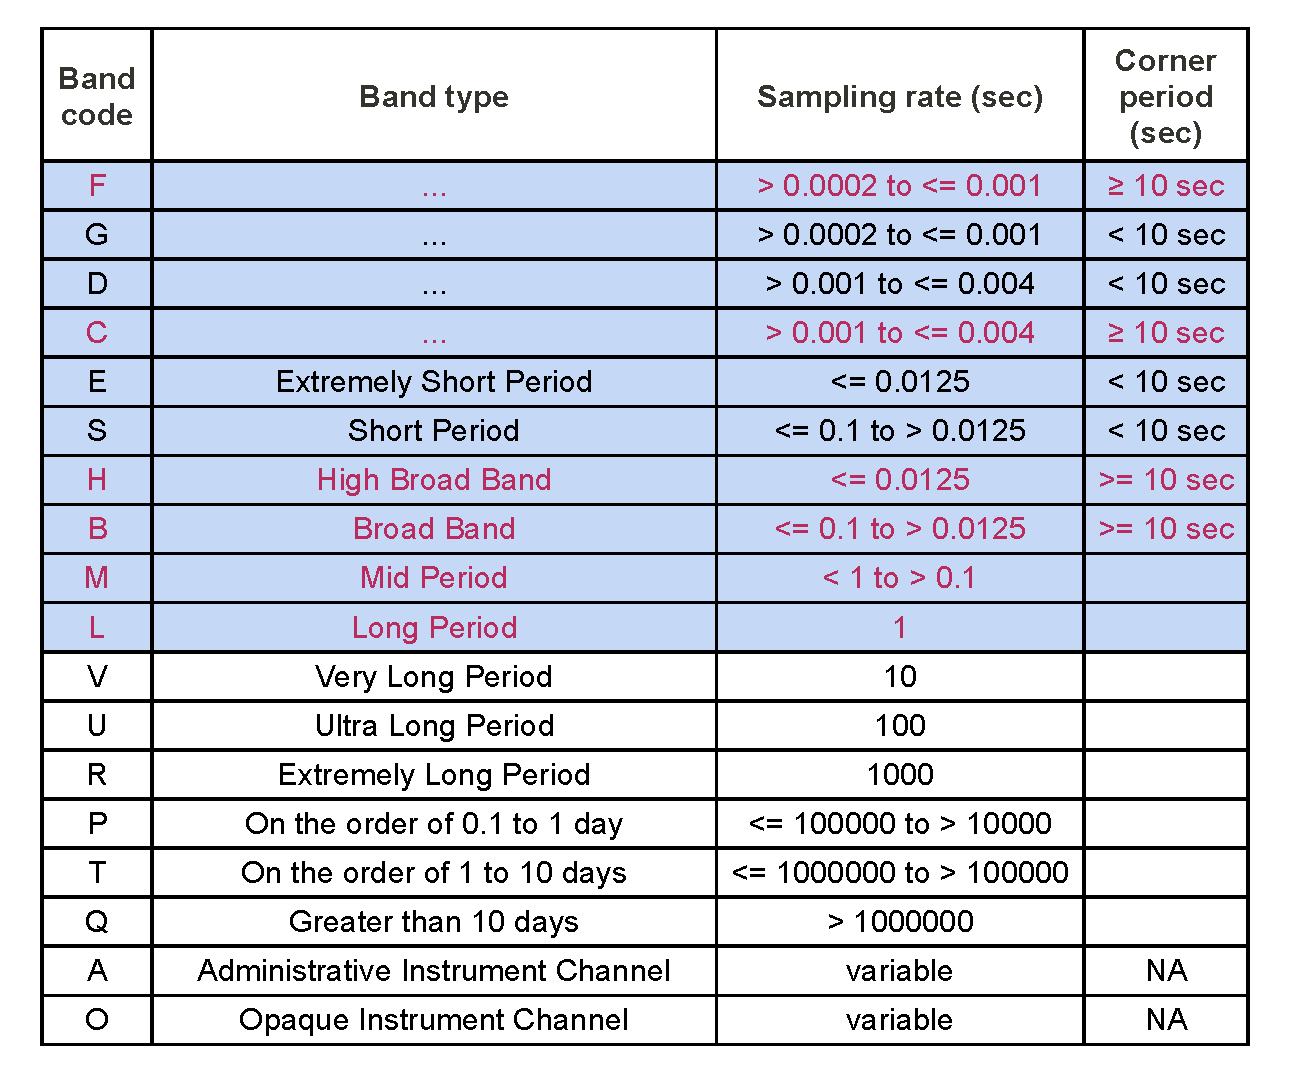
\includegraphics[scale=0.6]{figures/IRIS_band_codes}
\par\end{centering}

\caption{The band code convention is based on the sampling rate and the response
band of instruments. Please visit \texttt{www.iris.edu/manuals/SEED\_appA.htm}
for further information. Grey rows show the relative band-code range
in SPECFEM3D Cartesian, and the band codes used to name SEM seismograms
are denoted in red.}


\label{fig:IRIS_band_codes}
\end{figure}


\noindent \texttt{\textbf{Instrument code:}} The second letter in
the channel code corresponds to instrument codes, which specify the
family to which the sensor belongs. For instance, \texttt{H} and \texttt{L}
are used for high-gain and low-gain seismometers, respectively. The
instrument code of SEM seismograms will always be \texttt{X}, as assigned
by FDSN for synthetic seismograms. \\


\noindent \texttt{\textbf{Orientation code:}} The third letter in
channel codes is an orientation code, which generally describes the
physical configuration of the components of instrument packages. SPECFEM3D
Cartesian uses the traditional orientation code \texttt{E/N/Z} (East-West,
North-South, Vertical) for three components when a UTM projection
is used. If the UTM conversion is suppressed, i.e. the flag \texttt{SUPPRESS\_UTM\_PROJECTION}
is set to \texttt{.true.}, then the three components are labelled
\texttt{X/Y/Z} according to the Cartesian reference frame. \\


\noindent \texttt{\textbf{EXAMPLE:}} The sampling rate is given by
\texttt{DT} in the main parameter file \texttt{Par\_file} located
in the \texttt{DATA/} subdirectory. Depending on the resolution of
your simulations, if you choose a sampling rate greater than $0.01$
s and less than $1$ s, a seismogram recording displacements on the
vertical component of a station \texttt{ASBS} (network \texttt{AZ})
will be named \texttt{ASBS.AZ.MXZ.semd.sac}, whereas it will be \texttt{ASBS.AZ.BXZ.semd.sac},
if the sampling rate is greater than 0.0125 and less equal to 0.1
s.


\chapter{\label{cha:Troubleshooting}Troubleshooting}


\section*{FAQ}
\begin{description}
\item [{configuration fails:}]~


Examine the log file 'config.log'. It contains detailed informations.
In many cases, the paths to these specific compiler commands F90,
CC and MPIF90 will not be correct if `./configure` fails.


Please make sure that you have a working installation of a Fortran
compiler, a C compiler and an MPI implementation. You should be able
to compile this little program code:
\begin{lyxcode}
program~main~~~\\
~include~'mpif.h'~~~\\
~integer,~parameter~::~CUSTOM\_MPI\_TYPE~=~MPI\_REAL~~~\\
~integer~ier~~~\\
~call~MPI\_INIT(ier)~~~\\
~call~MPI\_BARRIER(MPI\_COMM\_WORLD,ier)~~~\\
~call~MPI\_FINALIZE(ier)~~~\\
~end
\end{lyxcode}
\item [{compilation fails stating:}] ~\\


\begin{lyxcode}
...~~~\\
~obj/program\_generate\_databases.o:~In~function~`MAIN\_\_':~~~\\
~program\_generate\_databases.f90:(.text+0x14):~undefined~reference~to~`\_gfortran\_set\_std'~~~\\
~...~~~\\

\end{lyxcode}

Make sure you're pointing to the right 'mpif90' wrapper command.


Normally, this message will appear when you are mixing two different
Fortran compilers. That is, using e.g. gfortran to compile non-MPI
files and mpif90, wrapper provided for e.g. ifort, to compile MPI-files.


fix: e.g. specify > ./configure FC=gfortran MPIF90=/usr/local/openmpi-gfortran/bin/mpif90

\item [{after executing \texttt{xmeshfem3D} I've got elements with skewness of 81\% percent, what does this mean:}] Look
at the skewness table printed in the \texttt{output\_mesher.txt} file
after executing \texttt{xmeshfem3D} for the example given in \texttt{examples/meshfem3D\_examples/simple\_model/}:

\begin{lyxcode}
...~~\\
~histogram~of~skewness~(0.~good~-~1.~bad):~~~\\
~0.0000000E+00~-~5.0000001E-02~27648~81.81818~\%~~~\\
~5.0000001E-02~-~0.1000000~0~0.0000000E+00~\%~~~\\
~...~~~\\

\end{lyxcode}

The first line means that you have 27,648 elements with a skewness
value between 0 and 0.05 (which means the element is basically not
skewed, just plain regular hexahedral element). The total number of
elements you have in this mesh is (see in the \texttt{output\_mesher.txt}
file a bit further down):
\begin{lyxcode}
...~~\\
~total~number~of~elements~in~entire~mesh:~33792~~~\\
~...~~~\\

\end{lyxcode}

which gives you that: 27,648 / 33,792 $\sim$ 81.8 \% of all elements
are not skewed, i.e. regular elements. a fantastic value :)


The histogram lists for this mesh also some stronger skewed elements,
for example the worst ones belong to:
\begin{lyxcode}
...~~\\
~0.6000000~-~0.6500000~2048~6.060606~\%~~~\\
~...~~~\\

\end{lyxcode}

about 6 \% of all elements have distortions with a skewness value
between 0.6 and 0.65. The skewness values give you a hint of how good
your mesh is. In an ideal world, you would want to have no distortions,
just like the 81\% from above. Those elements give you the best approximate
values by the GLL quadrature used in the spectral-element method.
However, having weakly distorted elements is still fine and the solutions
are still accurate enough. So empirically, values up to around 0.7
are tolerable, above that you should consider remeshing...


To give you an idea why some of the elements are distorted, see the
following figure \ref{fig:mesh.vp} of the mesh you obtain in the
example \texttt{examples/meshfem3D\_examples/simple\_model/}.
\begin{figure}[htbp]
\noindent \begin{centering}
\includegraphics[width=0.9\textwidth]{figures/mesh_vp}
\par\end{centering}

\caption{Paraview visualization using the mesh vtk-files for the example given
in \texttt{examples/meshfem3D\_examples/simple\_model/}.}


\label{fig:mesh.vp}
\end{figure}



You will see that the mesh contains a doubling layer, where we stitch
elements together such that the size of two elements will transition
to the size of one element (very useful to keep the ratio of wavespeed
/ element\_size about constant). Those elements in this doubling layer
have higher skewness values and make up those 6 \% in the histogram.

\item [{the code gives following error message "need at least one receiver":}] This
means that no stations given in the input file \texttt{DATA/STATIONS}
could be located within the dimensions of the mesh. This can happen
for example when the mesh was created with the in-house mesher \texttt{xmeshfem3D}
while using the Universal Transverse Mercator (UTM) projection but
the simulation with \texttt{xspecfem3D} was suppressing this projection
from latitude/longitude to x/y/z coordinates.


In such cases, try to change your \texttt{DATA/Par\_file} and set
e.g.:
\begin{lyxcode}
SUPPRESS\_UTM\_PROJECTION~=~.false.~~~\\

\end{lyxcode}

to be the same in \texttt{Mesh\_Par\_file} and \texttt{Par\_file}.
This flag should be identical when using the in-house mesher \texttt{xmeshfem3D},
\texttt{xgenerate\_databases} and \texttt{xspecfem3D} together to
run simulations.


The flag determines if the coordinates you specify for your source
and station locations are given as lat/lon degrees and must be converted
to UTM coordinates. As an example, if you use \texttt{.false.} within
\texttt{Mesh\_Par\_file} then you create a mesh with \texttt{xmeshfem3D}
using the UTM projection from lat/lon as input format to UTM projected
coordinates to store the mesh point positions, which is fine. The
error then may occur if in the \texttt{Par\_file} you have this set
to \texttt{.true.} so that the \texttt{xgenerate\_databases} and \texttt{xspecfem3D}
suppress the UTM projection and assume that all coordinates you use
now for source and receiver locations are given in meters (that is,
converted) already. So it won't find the specified locations in the
used mesh. As a solutions, just change the flag in \texttt{Par\_file}
to be the same as in \texttt{Mesh\_Par\_file} and rerun \texttt{xgenerate\_databases}
and \texttt{xspecfem3D} to make sure that your simulation works fine.

\item [{I get the following error message "forward simulation became unstable and blew up":}] In
most cases this means that your time step size \texttt{DT} is chosen
too big. Look at your files \texttt{output\_mesher.txt} or \texttt{output\_solver.txt}
created in the folder \texttt{OUTPUT\_FILES}. In these output files,
find the section:

\begin{lyxcode}
...~~~\\
~{*}{*}{*}{*}{*}{*}{*}{*}{*}{*}{*}{*}{*}{*}{*}{*}{*}{*}{*}{*}{*}{*}{*}{*}{*}{*}{*}{*}{*}{*}{*}{*}{*}{*}{*}{*}{*}{*}{*}{*}{*}{*}{*}{*}{*}~~~\\
~{*}{*}{*}~Verification~of~simulation~parameters~{*}{*}{*}~~~\\
~{*}{*}{*}{*}{*}{*}{*}{*}{*}{*}{*}{*}{*}{*}{*}{*}{*}{*}{*}{*}{*}{*}{*}{*}{*}{*}{*}{*}{*}{*}{*}{*}{*}{*}{*}{*}{*}{*}{*}{*}{*}{*}{*}{*}{*}~~~\\
~...~~~\\
~{*}{*}{*}~Minimum~period~resolved~=~4.308774~~~\\
~{*}{*}{*}~Maximum~suggested~time~step~=~6.8863556E-02~~~\\
~...~~~\\
~...~~~\\

\end{lyxcode}

then change \texttt{DT} in the \texttt{DATA/Par\_file} to be somewhere
close to the maximum suggested time step. In the example above: \\
 \texttt{DT = 0.05d0} \\
 would (most probably) work fine. It could be also bigger than the
0.068 s suggested. This depends a bit on the distortions of your mesh
elements. The more regular they are, the bigger you can choose \texttt{DT}.
Just play with this value a bit and see when the simulation becomes
stable ...

\end{description}

\chapter{\label{cha:License}License }

\textbf{GNU GENERAL PUBLIC LICENSE Version 2, June 1991. Copyright
(C) 1989, 1991 Free Software Foundation, Inc. 59 Temple Place, Suite
330, Boston, MA 02111-1307 USA} \\
 Everyone is permitted to copy and distribute verbatim copies of this
license document, but changing it is not allowed.


\section*{Preamble}

The licenses for most software are designed to take away your freedom
to share and change it. By contrast, the GNU General Public License
is intended to guarantee your freedom to share and change free software
-- to make sure the software is free for all its users. This General
Public License applies to most of the Free Software Foundation's software
and to any other program whose authors commit to using it. (Some other
Free Software Foundation software is covered by the GNU Library General
Public License instead.) You can apply it to your programs, too.

When we speak of free software, we are referring to freedom, not price.
Our General Public Licenses are designed to make sure that you have
the freedom to distribute copies of free software (and charge for
this service if you wish), that you receive source code or can get
it if you want it, that you can change the software or use pieces
of it in new free programs; and that you know you can do these things.

To protect your rights, we need to make restrictions that forbid anyone
to deny you these rights or to ask you to surrender the rights. These
restrictions translate to certain responsibilities for you if you
distribute copies of the software, or if you modify it.

For example, if you distribute copies of such a program, whether gratis
or for a fee, you must give the recipients all the rights that you
have. You must make sure that they, too, receive or can get the source
code. And you must show them these terms so they know their rights.

We protect your rights with two steps:
\begin{enumerate}
\item Copyright the software, and
\item Offer you this license which gives you legal permission to copy, distribute
and/or modify the software.
\end{enumerate}
Also, for each author's protection and ours, we want to make certain
that everyone understands that there is no warranty for this free
software. If the software is modified by someone else and passed on,
we want its recipients to know that what they have is not the original,
so that any problems introduced by others will not reflect on the
original authors' reputations.

Finally, any free program is threatened constantly by software patents.
We wish to avoid the danger that redistributors of a free program
will individually obtain patent licenses, in effect making the program
proprietary. To prevent this, we have made it clear that any patent
must be licensed for everyone's free use or not licensed at all.

The precise terms and conditions for copying, distribution and modification
follow.


\section*{GNU GENERAL PUBLIC LICENSE TERMS AND CONDITIONS FOR COPYING, DISTRIBUTION
AND MODIFICATION }
\begin{itemize}
\item 0.This License applies to any program or other work which contains
a notice placed by the copyright holder saying it may be distributed
under the terms of this General Public License. The ``Program''
below refers to any such program or work, and a ``work based on the
Program'' means either the Program or any derivative work under copyright
law: that is to say, a work containing the Program or a portion of
it, either verbatim or with modifications and/or translated into another
language. (Hereinafter, translation is included without limitation
in the term ``modification.'') Each licensee is addressed as ``you.''\\
 \\
 Activities other than copying, distribution and modification are
not covered by this License; they are outside its scope. The act of
running the Program is not restricted, and the output from the Program
is covered only if its contents constitute a work based on the Program
(independent of having been made by running the Program). Whether
that is true depends on what the Program does.\end{itemize}
\begin{enumerate}
\item You may copy and distribute verbatim copies of the Program's source
code as you receive it, in any medium, provided that you conspicuously
and appropriately publish on each copy an appropriate copyright notice
and disclaimer of warranty; keep intact all the notices that refer
to this License and to the absence of any warranty; and give any other
recipients of the Program a copy of this License along with the Program.


You may charge a fee for the physical act of transferring a copy,
and you may at your option offer warranty protection in exchange for
a fee.

\item You may modify your copy or copies of the Program or any portion of
it, thus forming a work based on the Program, and copy and distribute
such modifications or work under the terms of Section 1 above, provided
that you also meet all of these conditions:

\begin{enumerate}
\item You must cause the modified files to carry prominent notices stating
that you changed the files and the date of any change.
\item You must cause any work that you distribute or publish, that in whole
or in part contains or is derived from the Program or any part thereof,
to be licensed as a whole at no charge to all third parties under
the terms of this License.
\item If the modified program normally reads commands interactively when
run, you must cause it, when started running for such interactive
use in the most ordinary way, to print or display an announcement
including an appropriate copyright notice and a notice that there
is no warranty (or else, saying that you provide a warranty) and that
users may redistribute the program under these conditions, and telling
the user how to view a copy of this License. (Exception: if the Program
itself is interactive but does not normally print such an announcement,
your work based on the Program is not required to print an announcement.)
\end{enumerate}

These requirements apply to the modified work as a whole. If identifiable
sections of that work are not derived from the Program, and can be
reasonably considered independent and separate works in themselves,
then this License, and its terms, do not apply to those sections when
you distribute them as separate works. But when you distribute the
same sections as part of a whole which is a work based on the Program,
the distribution of the whole must be on the terms of this License,
whose permissions for other licensees extend to the entire whole,
and thus to each and every part regardless of who wrote it.


Thus, it is not the intent of this section to claim rights or contest
your rights to work written entirely by you; rather, the intent is
to exercise the right to control the distribution of derivative or
collective works based on the Program.


In addition, mere aggregation of another work not based on the Program
with the Program (or with a work based on the Program) on a volume
of a storage or distribution medium does not bring the other work
under the scope of this License.

\item You may copy and distribute the Program (or a work based on it, under
Section 2) in object code or executable form under the terms of Sections
1 and 2 above provided that you also do one of the following:

\begin{enumerate}
\item Accompany it with the complete corresponding machine-readable source
code, which must be distributed under the terms of Sections 1 and
2 above on a medium customarily used for software interchange; or,
\item Accompany it with a written offer, valid for at least three years,
to give any third party, for a charge no more than your cost of physically
performing source distribution, a complete machine-readable copy of
the corresponding source code, to be distributed under the terms of
Sections 1 and 2 above on a medium customarily used for software interchange;
or,
\item Accompany it with the information you received as to the offer to
distribute corresponding source code. (This alternative is allowed
only for noncommercial distribution and only if you received the program
in object code or executable form with such an offer, in accord with
Subsection b above.)
\end{enumerate}

The source code for a work means the preferred form of the work for
making modifications to it. For an executable work, complete source
code means all the source code for all modules it contains, plus any
associated interface definition files, plus the scripts used to control
compilation and installation of the executable. However, as a special
exception, the source code distributed need not include anything that
is normally distributed (in either source or binary form) with the
major components (compiler, kernel, and so on) of the operating system
on which the executable runs, unless that component itself accompanies
the executable.


If distribution of executable or object code is made by offering access
to copy from a designated place, then offering equivalent access to
copy the source code from the same place counts as distribution of
the source code, even though third parties are not compelled to copy
the source along with the object code.

\item You may not copy, modify, sublicense, or distribute the Program except
as expressly provided under this License. Any attempt otherwise to
copy, modify, sublicense or distribute the Program is void, and will
automatically terminate your rights under this License. However, parties
who have received copies, or rights, from you under this License will
not have their licenses terminated so long as such parties remain
in full compliance.
\item You are not required to accept this License, since you have not signed
it. However, nothing else grants you permission to modify or distribute
the Program or its derivative works. These actions are prohibited
by law if you do not accept this License. Therefore, by modifying
or distributing the Program (or any work based on the Program), you
indicate your acceptance of this License to do so, and all its terms
and conditions for copying, distributing or modifying the Program
or works based on it.
\item Each time you redistribute the Program (or any work based on the Program),
the recipient automatically receives a license from the original licensor
to copy, distribute or modify the Program subject to these terms and
conditions. You may not impose any further restrictions on the recipients'
exercise of the rights granted herein. You are not responsible for
enforcing compliance by third parties to this License.
\item If, as a consequence of a court judgment or allegation of patent infringement
or for any other reason (not limited to patent issues), conditions
are imposed on you (whether by court order, agreement or otherwise)
that contradict the conditions of this License, they do not excuse
you from the conditions of this License. If you cannot distribute
so as to satisfy simultaneously your obligations under this License
and any other pertinent obligations, then as a consequence you may
not distribute the Program at all. For example, if a patent license
would not permit royalty-free redistribution of the Program by all
those who receive copies directly or indirectly through you, then
the only way you could satisfy both it and this License would be to
refrain entirely from distribution of the Program.


If any portion of this section is held invalid or unenforceable under
any particular circumstance, the balance of the section is intended
to apply and the section as a whole is intended to apply in other
circumstances.


It is not the purpose of this section to induce you to infringe any
patents or other property right claims or to contest validity of any
such claims; this section has the sole purpose of protecting the integrity
of the free software distribution system, which is implemented by
public license practices. Many people have made generous contributions
to the wide range of software distributed through that system in reliance
on consistent application of that system; it is up to the author/donor
to decide if he or she is willing to distribute software through any
other system and a licensee cannot impose that choice.


This section is intended to make thoroughly clear what is believed
to be a consequence of the rest of this License.

\item If the distribution and/or use of the Program is restricted in certain
countries either by patents or by copyrighted interfaces, the original
copyright holder who places the Program under this License may add
an explicit geographical distribution limitation excluding those countries,
so that distribution is permitted only in or among countries not thus
excluded. In such case, this License incorporates the limitation as
if written in the body of this License.
\item The Free Software Foundation may publish revised and/or new versions
of the General Public License from time to time. Such new versions
will be similar in spirit to the present version, but may differ in
detail to address new problems or concerns.


Each version is given a distinguishing version number. If the Program
specifies a version number of this License which applies to it and
``any later version,'' you have the option of following the terms
and conditions either of that version or of any later version published
by the Free Software Foundation. If the Program does not specify a
version number of this License, you may choose any version ever published
by the Free Software Foundation.

\item If you wish to incorporate parts of the Program into other free programs
whose distribution conditions are different, write to the author to
ask for permission. For software which is copyrighted by the Free
Software Foundation, write to the Free Software Foundation; we sometimes
make exceptions for this. Our decision will be guided by the two goals
of preserving the free status of all derivatives of our free software
and of promoting the sharing and reuse of software generally.
\end{enumerate}

\subsection*{NO WARRANTY }
\begin{itemize}
\item 11.BECAUSE THE PROGRAM IS LICENSED FREE OF CHARGE, THERE IS NO WARRANTY
FOR THE PROGRAM, TO THE EXTENT PERMITTED BY APPLICABLE LAW. EXCEPT
WHEN OTHERWISE STATED IN WRITING THE COPYRIGHT HOLDERS AND/OR OTHER
PARTIES PROVIDE THE PROGRAM ``AS IS'' WITHOUT WARRANTY OF ANY KIND,
EITHER EXPRESSED OR IMPLIED, INCLUDING, BUT NOT LIMITED TO, THE IMPLIED
WARRANTIES OF MERCHANTABILITY AND FITNESS FOR A PARTICULAR PURPOSE.
THE ENTIRE RISK AS TO THE QUALITY AND PERFORMANCE OF THE PROGRAM IS
WITH YOU. SHOULD THE PROGRAM PROVE DEFECTIVE, YOU ASSUME THE COST
OF ALL NECESSARY SERVICING, REPAIR OR CORRECTION.
\item 12.IN NO EVENT UNLESS REQUIRED BY APPLICABLE LAW OR AGREED TO IN WRITING
WILL ANY COPYRIGHT HOLDER, OR ANY OTHER PARTY WHO MAY MODIFY AND/OR
REDISTRIBUTE THE PROGRAM AS PERMITTED ABOVE, BE LIABLE TO YOU FOR
DAMAGES, INCLUDING ANY GENERAL, SPECIAL, INCIDENTAL OR CONSEQUENTIAL
DAMAGES ARISING OUT OF THE USE OR INABILITY TO USE THE PROGRAM (INCLUDING
BUT NOT LIMITED TO LOSS OF DATA OR DATA BEING RENDERED INACCURATE
OR LOSSES SUSTAINED BY YOU OR THIRD PARTIES OR A FAILURE OF THE PROGRAM
TO OPERATE WITH ANY OTHER PROGRAMS), EVEN IF SUCH HOLDER OR OTHER
PARTY HAS BEEN ADVISED OF THE POSSIBILITY OF SUCH DAMAGES.
\end{itemize}

\section*{END OF TERMS AND CONDITIONS }


\subsection*{How to Apply These Terms to Your New Programs}

If you develop a new program, and you want it to be of the greatest
possible use to the public, the best way to achieve this is to make
it free software which everyone can redistribute and change under
these terms.

To do so, attach the following notices to the program. It is safest
to attach them to the start of each source file to most effectively
convey the exclusion of warranty; and each file should have at least
the ``copyright'' line and a pointer to where the full notice is
found. For example:
\begin{quote}
One line to give the program's name and a brief idea of what it does.
Copyright {\footnotesize $\copyright$ (}year) (name of author)

This program is free software; you can redistribute it and/or modify
it under the terms of the GNU General Public License as published
by the Free Software Foundation; either version 2 of the License,
or (at your option) any later version.

This program is distributed in the hope that it will be useful, but
WITHOUT ANY WARRANTY; without even the implied warranty of MERCHANTABILITY
or FITNESS FOR A PARTICULAR PURPOSE. See the GNU General Public License
for more details.

You should have received a copy of the GNU General Public License
along with this program; if not, write to the Free Software Foundation,
Inc., 59 Temple Place, Suite 330, Boston, MA 02111-1307 USA
\end{quote}
Also add information on how to contact you by electronic and paper
mail.

If the program is interactive, make it output a short notice like
this when it starts in an interactive mode:
\begin{quote}
Gnomovision version 69, Copyright $\copyright$ year name of author
Gnomovision comes with ABSOLUTELY NO WARRANTY; for details type `show
w'. This is free software, and you are welcome to redistribute it
under certain conditions; type `show c' for details.
\end{quote}
The hypothetical commands `show w' and `show c' should show the appropriate
parts of the General Public License. Of course, the commands you use
may be called something other than `show w' and `show c'; they could
even be mouse-clicks or menu items -- whatever suits your program.

You should also get your employer (if you work as a programmer) or
your school, if any, to sign a ``copyright disclaimer'' for the
program, if necessary. Here is a sample; alter the names:
\begin{quote}
Yoyodyne, Inc., hereby disclaims all copyright interest in the program
`Gnomovision' (which makes passes at compilers) written by James Hacker.

(signature of Ty Coon)\\
 1 April 1989 \\
 Ty Coon, President of Vice
\end{quote}
This General Public License does not permit incorporating your program
into proprietary programs. If your program is a subroutine library,
you may consider it more useful to permit linking proprietary applications
with the library. If this is what you want to do, use the GNU Library
General Public License instead of this License.
\end{document}
